  % interacttfssample.tex
% v1.05 - August 2017

\documentclass[dvipdfmx]{interact}

%\usepackage{epstopdf}% To incorporate .eps illustrations using PDFLaTeX, etc.
%\usepackage[caption=false]{subfig}% Support for small, `sub' figures and tables
%\usepackage[nolists,tablesfirst]{endfloat}% To `separate' figures and tables from text if required
\usepackage[format=hang]{caption}
\usepackage[format=hang, subrefformat=parens]{subcaption}
\captionsetup{compatibility=false}
\usepackage{algorithm}
\usepackage{algorithmic}
\usepackage{hyperref}
\usepackage{amsmath,amssymb}

%\usepackage[doublespacing]{setspace}% To produce a `double spaced' document if required
%\setlength\parindent{24pt}% To increase paragraph indentation when line spacing is doubled
%\setlength\bibindent{2em}% To increase hanging indent in bibliography when line spacing is doubled

\usepackage[numbers,sort&compress]{natbib}% Citation support using natbib.sty
\bibpunct[, ]{[}{]}{,}{n}{,}{,}% Citation support using natbib.sty
\renewcommand\bibfont{\fontsize{10}{12}\selectfont}% Bibliography support using natbib.sty

\theoremstyle{plain}% Theorem-like structures provided by amsthm.sty
\newtheorem{theorem}{Theorem}[section]
\newtheorem{lemma}[theorem]{Lemma}
\newtheorem{corollary}[theorem]{Corollary}
\newtheorem{proposition}[theorem]{Proposition}

\theoremstyle{definition}
\newtheorem{definition}[theorem]{Definition}
\newtheorem{example}[theorem]{Example}

\theoremstyle{remark}
\newtheorem{remark}{Remark}
\newtheorem{notation}{Notation}

\newtheoremstyle{problemstyle}  % <name>
        {3pt}                                               % <space above>
        {3pt}                                               % <space below>
        {\normalfont}                               % <body font>
        {}                                                  % <indent amount}
        {\bfseries\itshape}                 % <theorem head font>
        {\normalfont\bfseries:}         % <punctuation after theorem head>
        {.5em}                                          % <space after theorem head>
        {}                                                  % <theorem % head spec (can be left empty, meaning `normal')>
\theoremstyle{problemstyle}

\newtheorem{problem}{Problem}[section] % Comment out [section] to remove section number dependence


\begin{document}

%\articletype{ARTICLE TEMPLATE}% Specify the article type or omit as appropriate

\title{Polyhedra with Spherical Faces and Four-Dimensional Kleinian Groups}

\author{
\name{Kento Nakamura \textsuperscript{a}\thanks{CONTACT
Kento Nakamura. Email: somaarcr@gmail.com Web: soma-arc.net}, Yoshiaki Araki \textsuperscript{b}
 and Kazushi Ahara\textsuperscript{c}}
\affil{\textsuperscript{a}Graduate School of Advanced Mathematical
Sciences, Meiji University, Tokyo, Japan; 
\textsuperscript{b}Japan Tessellation Design Association, President;\\
\textsuperscript{c}School of Interdisciplinary Mathematical Sciences
, Meiji University, Tokyo, Japan.}
}

\maketitle

\begin{abstract}
 これまで,球面体群について,提案され
 このフラクタルは豊かな図像を見せる.
 元来,多大な時間がかかっていた.しかし,ハードウェアの進化とアルゴリズ
 ムによってリアルタイムに図を描画できるようになった.
 本論文では可視化された図像から数学的問題を提起し,解決する.
 その問題は...であり,...を示す.

 We are interested in finding examples of quasi-fuchsian subgroup of
 M\"ob$(S^3)$, the group of orientation preserving M\"obius
 transformations on $S^3$. In this article we consider a new problem of
 Euclidian geometry about polyhedra with spherical faces and we obtain
 interesting examples of quasi-fuchsian groups and pictures of fractal
 two-spheres.

 Usually, rendering image of the fractals takes much time.
 We use an original algorithm Iterated Inversion System (IIS.)
 and sphere tracing, a kind of a ray tracing techniques.
 We can render the images of fractals in real-time.
 In this paper we focus visualized images.
 We find mathematical problem from rendered images.
\end{abstract}

\begin{keywords}
mathematics; visualization; fractals; Kleinian groups; circle inversion;
 sphere inversion
\end{keywords}

\tableofcontents

\section{Introduction}

\begin{figure}[h!tbp]
  \begin{minipage}[t]{0.25\textwidth}
   \centering
   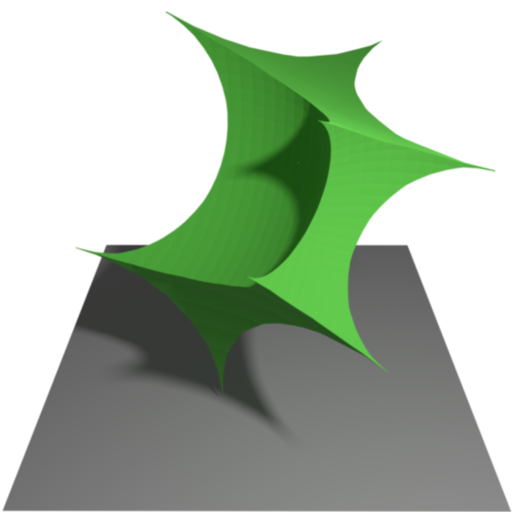
\includegraphics[height=1.2in, keepaspectratio]{./img/introduction/cube.png}
   \caption{Cube-type sphairahedron.}
   \label{fig:cubeSphaira}
  \end{minipage}
  \hspace*{\fill}
 \begin{minipage}[t]{0.75\textwidth}
  \begin{minipage}[t]{0.25\textwidth}
   \centering
   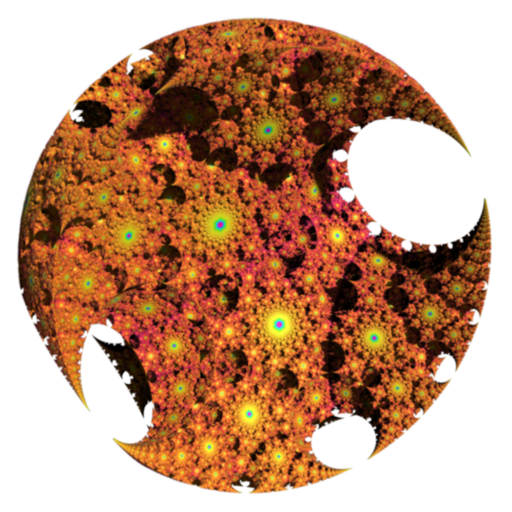
\includegraphics[height=1.2in,
   keepaspectratio]{./img/introduction/quasi-sphere.png}
   \subcaption{}
  \end{minipage}
  \hspace*{\fill}
  \begin{minipage}[t]{0.25\textwidth}
   \centering
   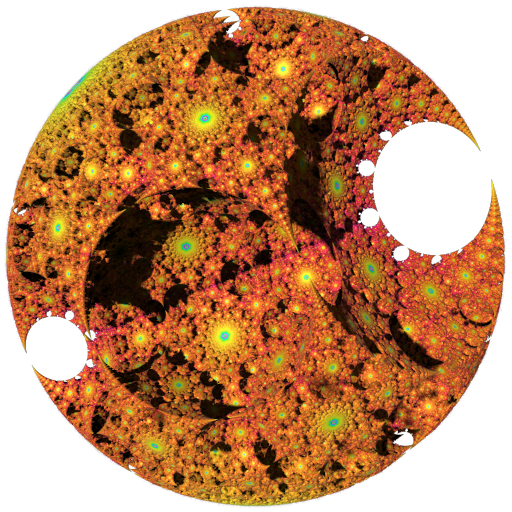
\includegraphics[height=1.2in,
   keepaspectratio]{./img/introduction/other.png}
   \subcaption{}
  \end{minipage}
  \hspace*{\fill}
  \begin{minipage}[t]{0.25\textwidth}
   \centering
   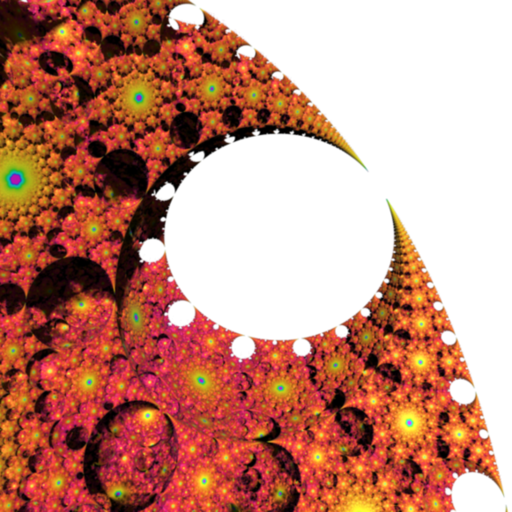
\includegraphics[height=1.2in,
   keepaspectratio]{./img/introduction/quasi-sphereZoom.png}
   \subcaption{}
  \end{minipage}
  \hspace*{\fill}
  \caption{Images of a quasi-sphere rendered in different viewpoints.}
  \label{fig:quasi-sphere}
 \end{minipage}
\end{figure}

\subsection{Background}

In this paper, we deal with geometrical concept called
\textit{Sphairahedron}. Sphairahedron is invented by Kazushi Ahara and
Yoshiaki Araki \cite{AharaAraki} in 2003. Sphairahedron is a coined word
combining two words sphaira- (a prefix that means 'spherical') and
-hedron (a suffix comes from 'polyhedron.') It looks like a polyhedron
with spherical faces. See Figure \ref{fig:cubeSphaira}. It shows cube-type
sphairahedron. As we can see, each face of the cube is a part of a
sphere.

Moreover, we can make a tiling pattern of sphairahedra using inversions
of each spherical faces. In many cases, the boundary of the tiling
patterns converges to three-dimensional fractal structure. 
The union of all the tiles is mostly homeomorphic to a three-dimensional
ball. Thus, this is called a \textit{quasi-sphere} and shown in Figure
\ref{fig:quasi-sphere}.
Quasi-sphere has complicated and beautiful fractal structures.
So, it interested fractal art community because it is beginning of
the complicated three-dimensional fractal.

In spite of innovative idea, there are few publications
\cite{AharaAraki}\cite{AharaJa}.
After Ahara and Araki publish two articles, the research of the
sphairahedra stop. 
One of the reasons is that it takes too much time to render the image of
the quasi-sphere with the computer in those days.

After that Ryo Kageyama perform further experiment of
cube-type sphairahedron in his master thesis \cite{kageyama}. 
He use a geometrical concept called \textit{lens} to study sphairahedra. 

In 2017, breakthrough is came out. We develop an algorithm called
\textit{Iterated Inversion System (IIS)} to visualize fractals based on
inversions in circles or spheres.
Combining IIS and \textit{Sphere tracing}, a kind of ray tracing
technique, we can render image of quasi-sphere in real time.
For more details of this algorithm, see
\cite{bridges2016} or \cite{bridges2017}.

The our previous paper \cite{bridges2018} is focused on the artistical
perspective of the sphairahedron and its fractals.
In this article we introduce mathematical details,
mathematical problems, and its solutions. 

There are pictures of three-dimensional, so it is hard to see whole
appearance only by them. We can see sphairahedron based fractal renderer,
 more pictures and more movies in the
our web site\footnote{\url{https://sphairahedron.net}}.

\subsection{Sphairahedron}

\begin{figure}[h!tbp]
 \begin{minipage}[t]{0.6\textwidth}
  \centering
  \begin{minipage}[t]{0.19\textwidth}
   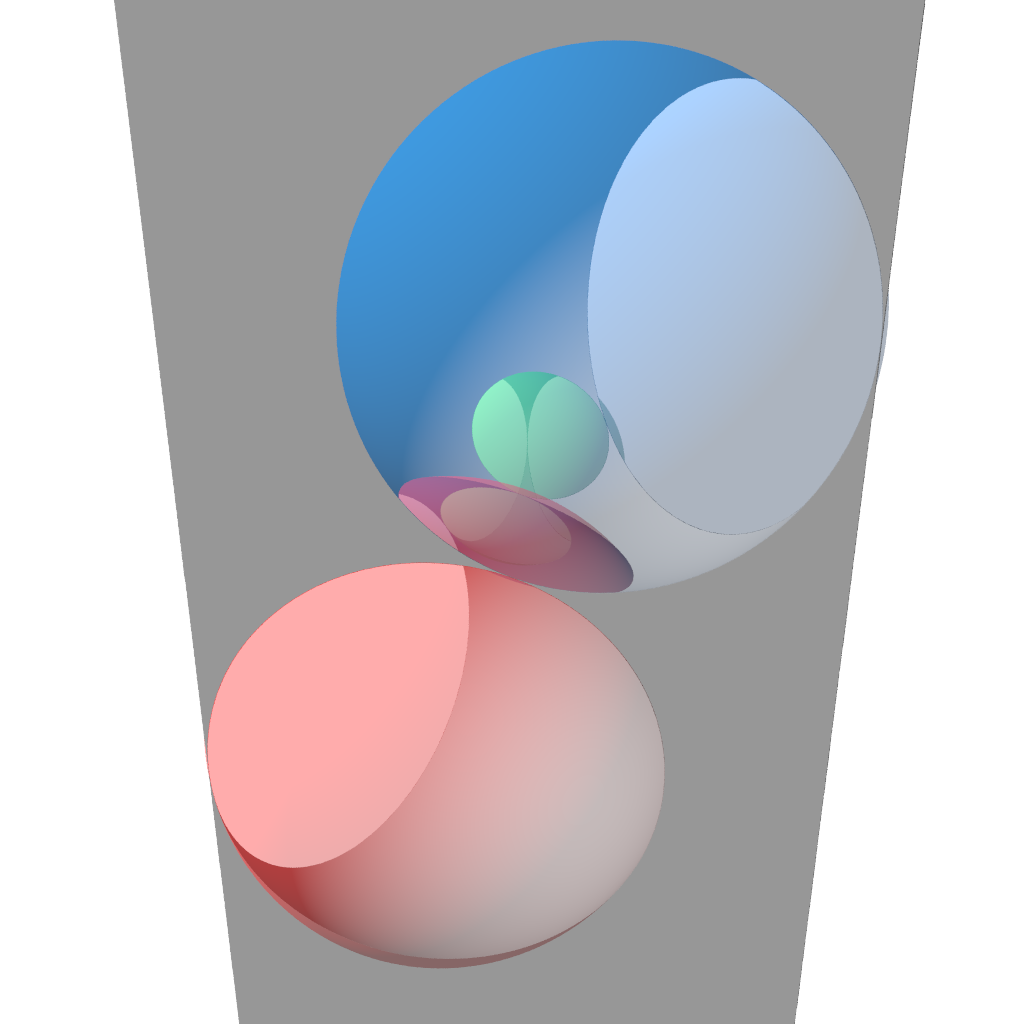
\includegraphics[width=1.2in, height=1.2in, keepaspectratio]
   {./img/sphairahedralPrism/sphairaAll.png}
   \subcaption{$A$}
   \label{fig:sphairaPrismAll}
  \end{minipage}
  \hspace*{\fill}
  \begin{minipage}[t]{0.19\textwidth}
   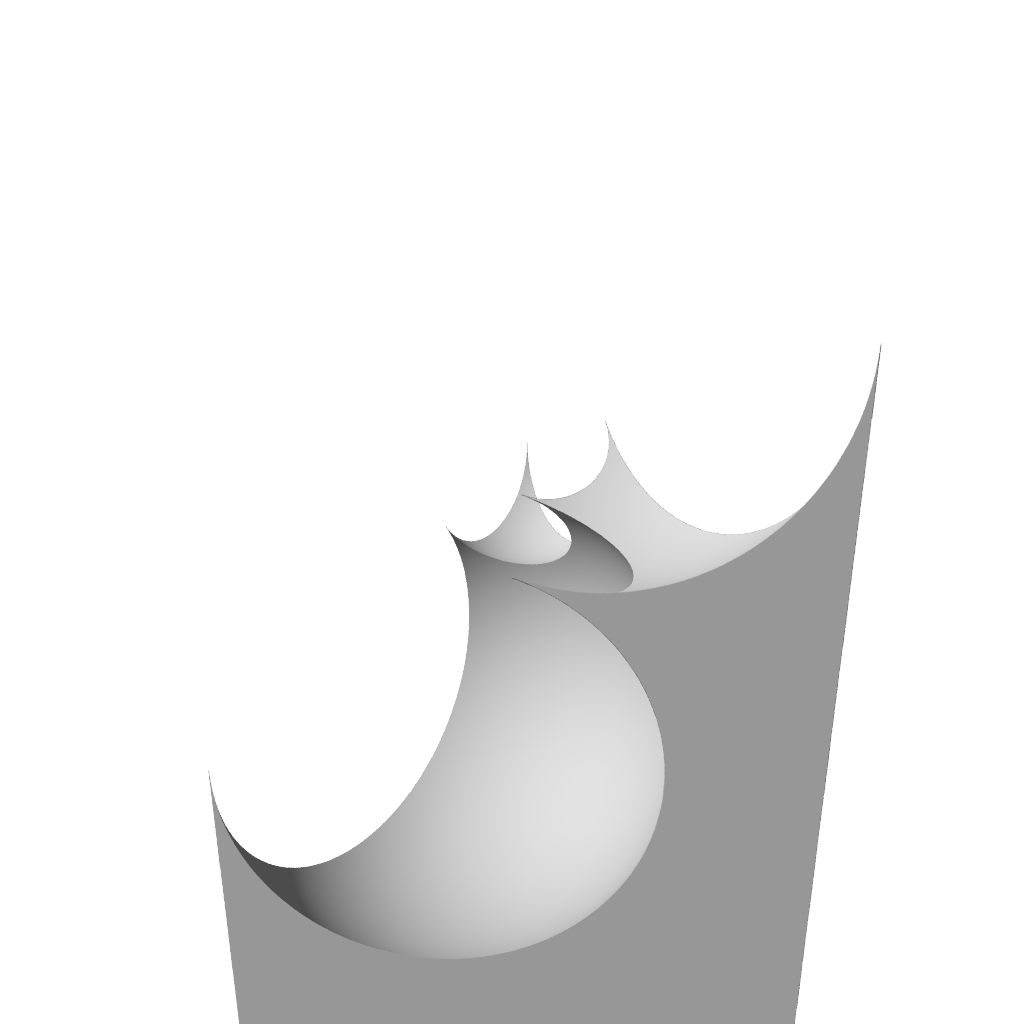
\includegraphics[width=1.2in, height=1.2in, keepaspectratio]
   {./img/sphairahedralPrism/sphairaHalf.png}
   \subcaption{Infinite type}
   \label{fig:sphairaPrismHalf}
  \end{minipage}
  \hspace*{\fill}
  \begin{minipage}[t]{0.19\textwidth}
   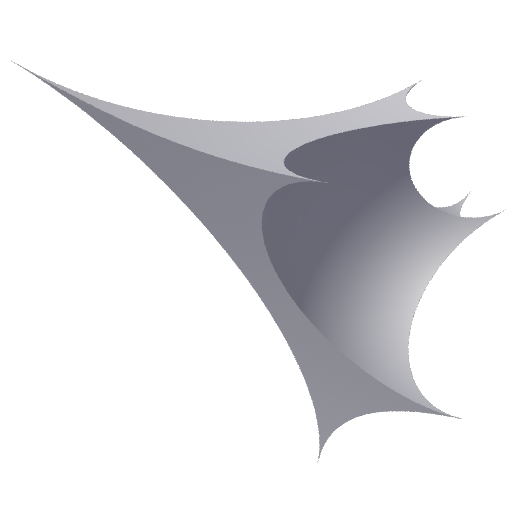
\includegraphics[width=1.2in, height=1.2in,
   keepaspectratio]{./img/sphairahedralPrism/sphairahedron.png} 
   \subcaption{Finite type}
   \label{fig:sphairahedronFinite}
  \end{minipage}
  \hspace*{\fill}
  \caption{Sphairahedron.}
  \label{fig:sphairahedron}
 \end{minipage}
 \begin{minipage}[t]{0.4\textwidth}
  \centering
  \begin{minipage}[t]{0.19\textwidth}
   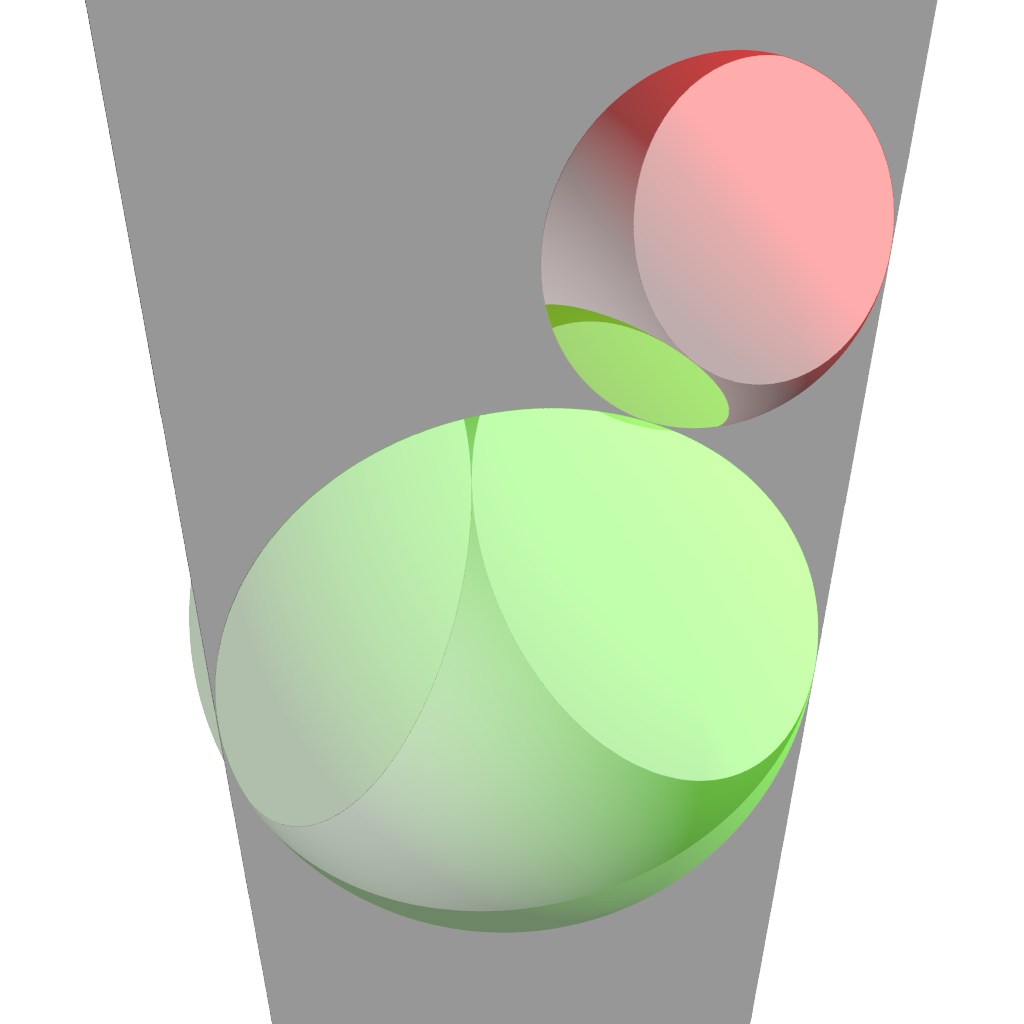
\includegraphics[width=1.2in, height=1.2in,
   keepaspectratio]{./img/sphairahedralPrism/semiSphairaAll.png}
   \subcaption{$A$}
   \label{fig:semi-sphairaAll}
  \end{minipage}
  \hspace*{\fill}
  \begin{minipage}[t]{0.19\textwidth}
   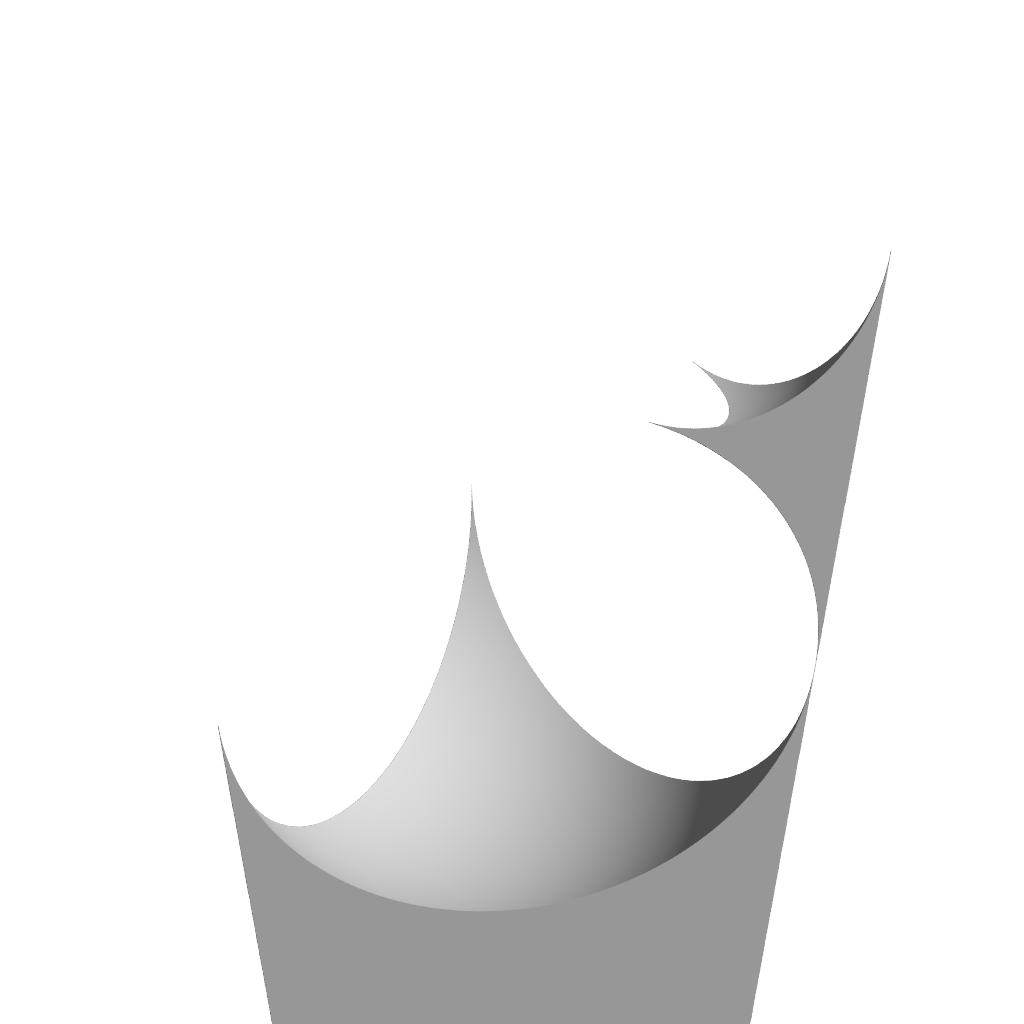
\includegraphics[width=1.2in, height=1.2in,
   keepaspectratio]{./img/sphairahedralPrism/semiSphairaHalf.png}
   \subcaption{Infinite type}
   \label{fig:semi-sphairaHalf}
  \end{minipage}
  \hspace*{\fill}
  \caption{Semi-sphairahedron.}
  \label{fig:semi-sphairahedron}
 \end{minipage}
\end{figure}

\begin{figure}[h!tbp]
  \centering
 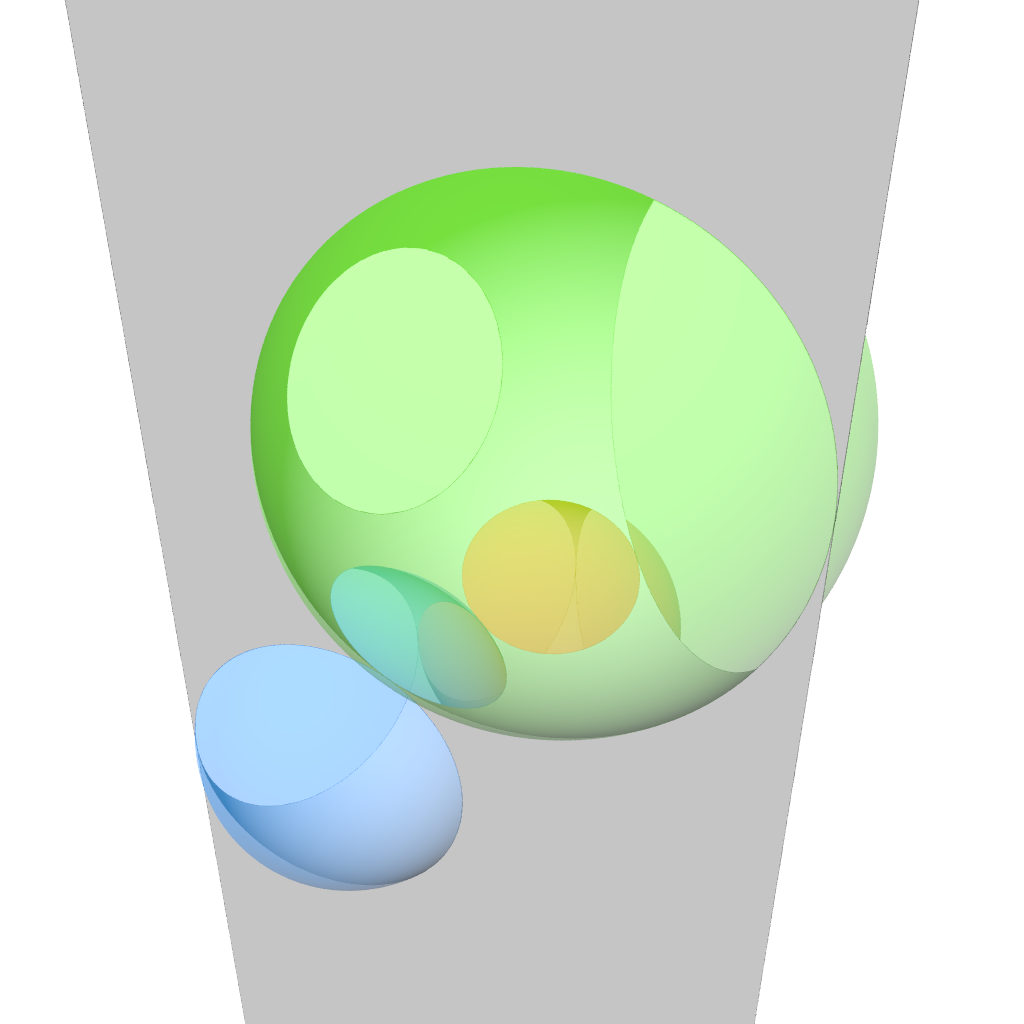
\includegraphics[width=1.2in, height=1.2in,
 keepaspectratio]{./img/sphairahedralPrism/hole.png}
 \caption{sphairahedron with hole.}
  \label{fig:brokenHole}
\end{figure}

We will describe the simple definition of a sphairahedron used in \cite{bridges2018}.
First of all, let $S^3 = R^3 \cup \{\infty\}$ be a three-dimensional sphere and let
$\overline{D_1},~\overline{D_2},~...,~\overline{D_p}$ be some
three-dimensional closed balls.
We consider the complement $A$ of the union of these balls, that is,
$A = S^3 - (\overline{D_1} \cup \overline{D_2} \cup ... \cup \overline{D_p})$.
If $A$ is composed of simply-connected two components;
in other words, $A$ has two connected components and the first homology
group of each component is trivial, we call one side of $A$
a sphairahedron.

The image in Figure \ref{fig:sphairahedron}\subref{fig:sphairaPrismAll}
is an example of $A$.
We hollow out the $S^3$ with six balls: we remove three half space
(three balls with infinite radius,) from $S^3$ and obtain the prism of
infinite length, and we scoop out the prism by the remaining
three-colored transparent balls as in Figure
\ref{fig:sphairahedron}\subref{fig:sphairaPrismAll}.
$A$ is composed of two parts, and each of the components is simply connected.
Since it has six faces, and these faces are arranged as those of faces of
a cube, it is called a cube-type sphairahedron.
Especially, the sphairahedron shown in Figure 
\ref{fig:sphairahedron}\subref{fig:sphairaPrismHalf}
is also called an \textit{infinite type sphairahedron},
because one of the vertices of the sphairahedron is at the infinity.
Similarly, the shape hollowed out by six finite balls in Figure
\ref{fig:sphairahedron}\subref{fig:sphairahedronFinite} is called a
\textit{finite type sphairahedron}.

Moreover, we can loosen the definition of sphairahedron,
that is, the case $A$ has simply connected three or more components.
Figure \ref{fig:semi-sphairahedron}\subref{fig:semi-sphairaAll} shows an
example of $A$ with simply connected three components.
It is the $S^3$ scooped out by five balls and a pentahedral prism type
sphairahedron.
We divide $A$ so that one part of $A$ has five faces as shown in
Figure \ref{fig:semi-sphairahedron}\subref{fig:semi-sphairaHalf}.
We can regard the resulting shape as a singular case of a pentahedron,
and we call it a \textit{semi-sphairahedron}.
When Ahara, Araki and Kageyama did not deal with semi-sphairahedron and
did not render its tiling patterns.

When the sphairahedron is not discrete, the sphairahedron is broken.
For example, it has unnecessary hole and so on.
See Figure \ref{fig:brokenHole}. It shows broken sphairahedron.
The green sphere make a hole.

\subsection{Construct Fractal}

\begin{figure}[H]
 \begin{minipage}[t]{0.19\textwidth}
  \centering
  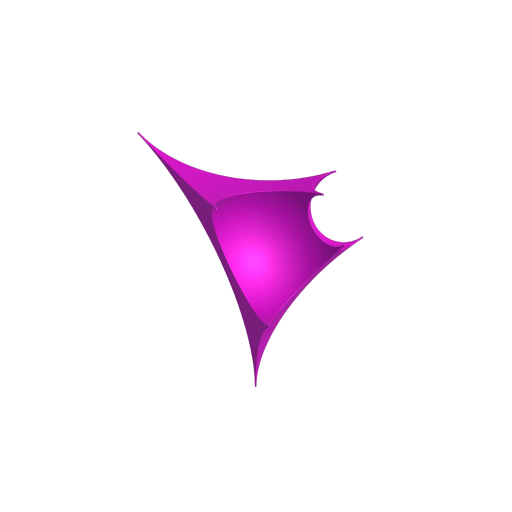
\includegraphics[width=1.1in, height=1.1in, keepaspectratio]{./img/constructFractal/finiteProcess/step1.png}
  \subcaption{Step 1}
  \label{fig:sphaira-step1}
 \end{minipage}
 \hspace*{\fill}
 \begin{minipage}[t]{0.19\textwidth}
  \centering
  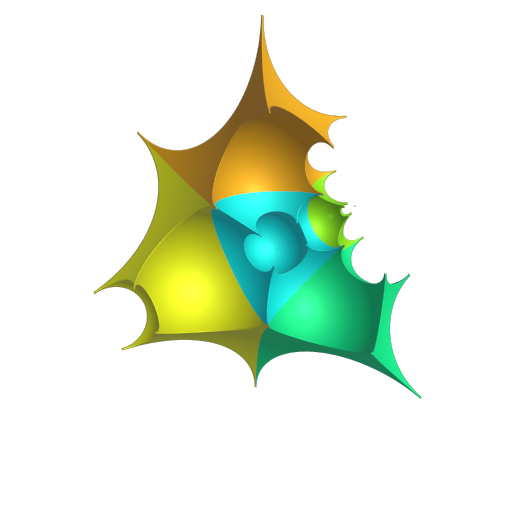
\includegraphics[width=1.1in, height=1.1in, keepaspectratio]{./img/constructFractal/finiteProcess/step2.png}
  \subcaption{Step 2}
  \label{fig:sphaira-step2}
 \end{minipage}
 \hspace*{\fill}
 \begin{minipage}[t]{0.19\textwidth}
  \centering
  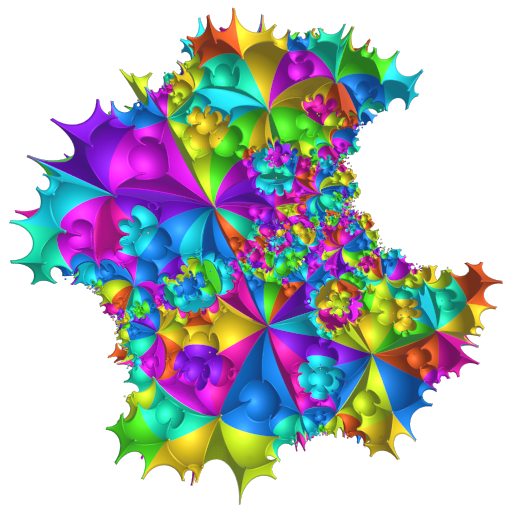
\includegraphics[width=1.1in, height=1.1in, keepaspectratio]{./img/constructFractal/finiteProcess/step5.png}
  \subcaption{Step 5}
  \label{fig:sphaira-step5}
 \end{minipage}
 \hspace*{\fill}
 \begin{minipage}[t]{0.19\textwidth}
  \centering
  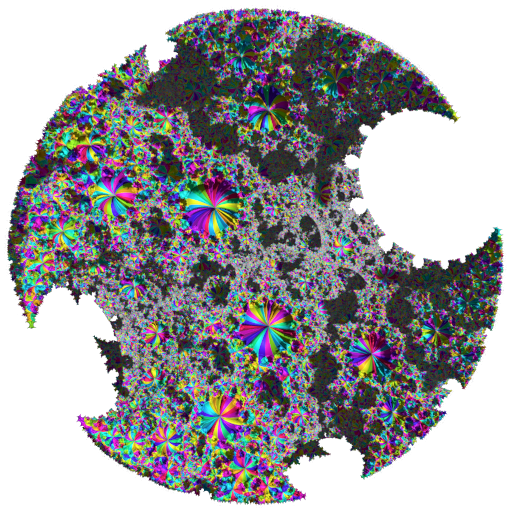
\includegraphics[width=1.1in, height=1.1in, keepaspectratio]{./img/constructFractal/finiteProcess/step10.png}
  \subcaption{Step 10}
  \label{fig:sphaira-step10}
 \end{minipage}
 \hspace*{\fill}
 \begin{minipage}[t]{0.19\textwidth}
  \centering
  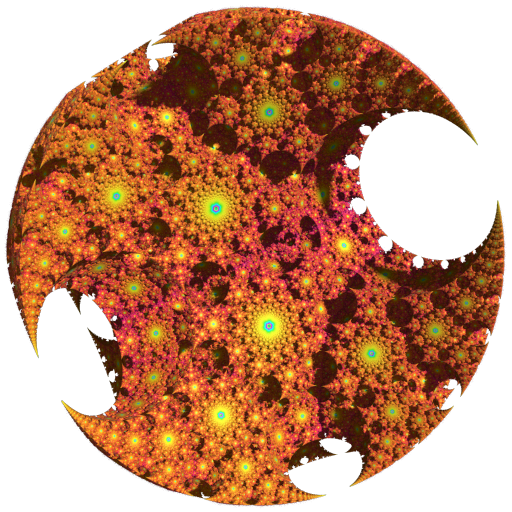
\includegraphics[width=1.1in, height=1.1in, keepaspectratio]{./img/constructFractal/finiteProcess/final.png}
  \subcaption{Final image}
  \label{fig:sphaira-final}
 \end{minipage}
 \hspace*{\fill}
 \caption{Tiling of a finite cube-type sphairahedron.}
 \label{fig:sphairahedronTile}
\end{figure}

\begin{figure}[h!tbp]
 \begin{minipage}[t]{0.19\textwidth}
  \centering
  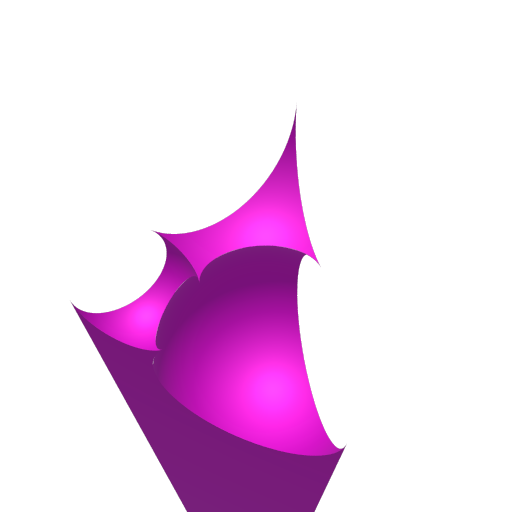
\includegraphics[height=1.2in, keepaspectratio]{./img/constructFractal/terrainProcess/step1.png}
  \subcaption{Step 1}
  \label{fig:terrainStep1}
 \end{minipage}
 \hspace*{\fill}
 \begin{minipage}[t]{0.19\textwidth}
  \centering
  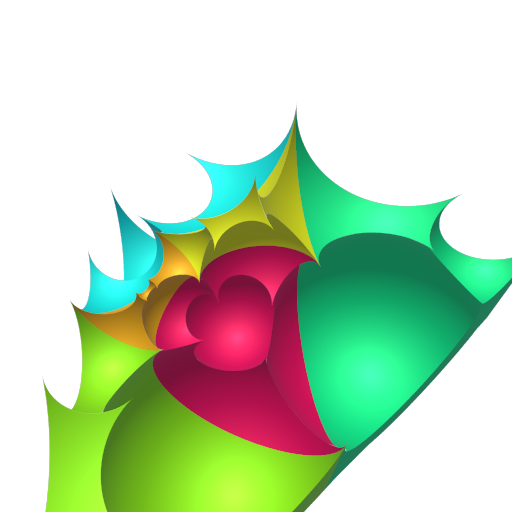
\includegraphics[height=1.2in, keepaspectratio]{./img/constructFractal/terrainProcess/step2.png}
  \subcaption{Step 2}
  \label{}
 \end{minipage}
 \hspace*{\fill}
 \begin{minipage}[t]{0.19\textwidth}
  \centering
  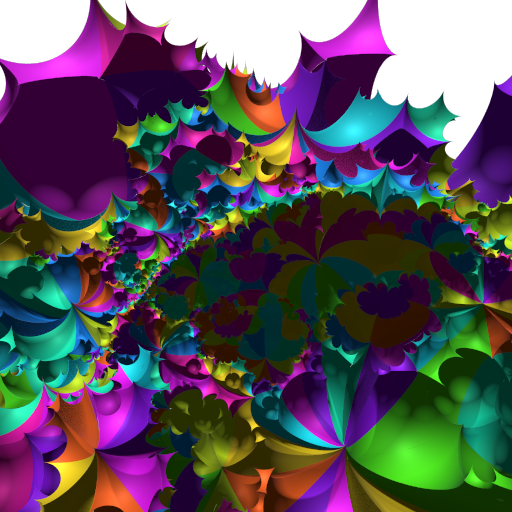
\includegraphics[height=1.2in, keepaspectratio]{./img/constructFractal/terrainProcess/step5.png}
  \subcaption{Step 5}
  \label{}
 \end{minipage}
 \hspace*{\fill}
 \begin{minipage}[t]{0.19\textwidth}
  \centering
  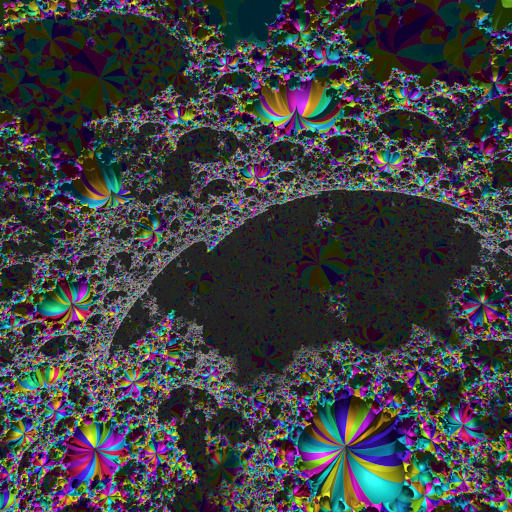
\includegraphics[height=1.2in, keepaspectratio]{./img/constructFractal/terrainProcess/step10.jpg}
  \subcaption{Step 10}
  \label{fig:terrainStep10}
 \end{minipage}
 \hspace*{\fill}
 \begin{minipage}[t]{0.19\textwidth}
  \centering
  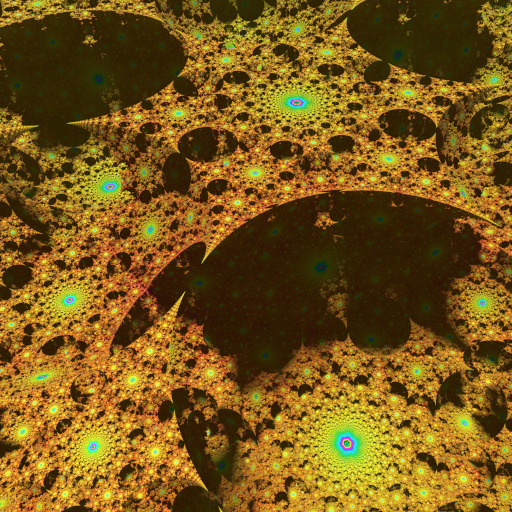
\includegraphics[height=1.2in, keepaspectratio]{./img/constructFractal/terrainProcess/final.jpg}
  \subcaption{Final image}
  \label{fig:sphairaPrismFinal}
 \end{minipage}
 \caption{Tiling of a cube-type infinite sphairahedron.}
 \label{fig:sphairahedralPrismTile}
\end{figure}

\begin{figure}[h!tbp]
  \centering
 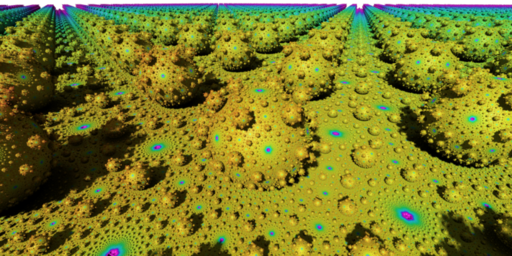
\includegraphics[width=1.2in, height=1.2in,
 keepaspectratio]{./img/constructFractal/semi-terrain2.png}
 \caption{sphairahedron with hole.}
  \label{fig:semiSphairaSpheres}
\end{figure}

In Figure \ref{fig:sphairahedronTile}, we show a process of the tiling of
sphairahedra.
The sphairahedron shown in Figure
\ref{fig:sphairahedronTile}\subref{fig:sphaira-step1} has six spherical
faces.
We apply inversions in each spherical face to original sphairahedron,
and we obtain new six sphairahedra surrounding the initial sphairahedron
as shown in Figure
\ref{fig:sphairahedronTile}\subref{fig:sphaira-final}.
Next, we apply inversions in each of the new faces to the new sphairahedra,
and we obtain more sphairahedra.
We continue iterating inversions, and finally, we get a three-dimensional
fractal shape as presented in Figure
\ref{fig:sphairahedronTile}\subref{fig:sphaira-final}.

Also, an infinite type sphairahedron can be tiled as presented in Figure
\ref{fig:sphairahedralPrismTile}.
The pattern converges to fractal terrain owing to reflections over side
faces of the sphairahedron as shown in Figure 
\ref{fig:sphairahedralPrismTile}\subref{fig:terrainStep1}.
In the fractal terrain, we can find symmetry easily.
For example, we can see hexagram-like terrain patterns in Figure
\ref{fig:sphairahedralPrismTile}\subref{fig:sphairaPrismFinal}.
These patterns are originated from the dihedral angles of the side faces of
$\pi / 3$.

In the same way as the tiling of the sphairahedron, a semi-sphairahedron
can be tiled by the inversions about its faces.
The resulting fractal of the semi-sphairahedron is different from normal
sphairahedron's one.
Figure \ref{fig:semiSphairaSpheres} shows the pattern
generated by an infinite semi-sphairahedron shown in Figure 
\ref{fig:semi-sphairahedron}\subref{fig:semi-sphairaHalf}.
It is the union of an infinite number of balls
circumscribing each other and no longer homeomorphic
to a three-dimensional ball.
Thus, It is not a quasi-sphere or a quasi-fuchsian.
We will describe more about a tiling pattern of a semi-sphairahedron later.

In the images of fractals within this paper, each tile of the
sphairahedra is colored according to the
number of inversions.
We use the color wheel to determine their color,
and the tile's color varies in order of red, yellow, green, and blue.
In Figure \ref{fig:sphairahedronTile}\subref{fig:sphaira-step1} $\sim$ \subref{fig:sphaira-step10} and
Figure \ref{fig:sphairahedralPrismTile}\subref{fig:terrainStep1} $\sim$ \subref{fig:terrainStep10},
we refer color wheel with large steps to visualize each tile clearly.
On the other hand, in the other images, we refer the wheel with smaller
steps, and we find lots of tiles with many inversions in the blue
parts of the fractal.
We can also find that the blue parts themselves form the constant
patterns.

Up to this point, we showed tiling patterns without gaps between the tiles and
intersections of the tiles.
However, not every sphairahedra can generate such proper tiling patterns.
To obtain them, we have to consider two mathematical properties
of the original sphairahedron, that is, the sphairahedron should be
ideal and rational.
In the following sections, we will introduce these properties and parameter
space for the ideal rational sphairahedron.


\section{Compute Parameter Space of Ideal Rational Sphairahedra}

\subsection{Introduction of Group $G$}

We are interested in finding examples of quasi-fuchsian sub-group of
M\"ob$_{+}(S^3)$, the group of orientation preserving M\"obius
transformation on $S^3 = R^3 \bigcup \{\infty\}$. For a subgroup $G$ of
Mob$_+(S^3)$, let the discontinuity set $\Omega(G)$ be
$$
\Omega(G) = \left\{ x \in S^3 \left| \hspace{1mm} 
\begin{minipage}{8cm}
the point x possesses a neighborhood $(x)$
such that the intersection $U(x) \cap gU(x)$ is empty for all but finite
elements $g\in G$
\end{minipage}
 \right. \right\}.
$$
The complement $\Lambda(G) := S^3 \backslash \Omega(G)$ is called the
limit set of the group $G$. $G$ is a Kleinian group if $\Omega(G)$ is
not empty. The limit set $\Lambda(G)$ consists either of 0 or 1 or 2 or
infinitely many points. Here we consider only the case that $\Lambda$
is infinite and two-dimensional. A Kleinian group $G$ is a fuchsian
group if $\Lambda(G)$ is a closed round sphere. $G$ is called a
quasi-fuchsian group is $\Lambda(G)$ is homeomorphic to a closed sphere
and there exits a homeomorphism $f:S^3 \rightarrow S^3$ which conjugates
$G$ to a fuchsian group. If $G$ is a quasi-fuchsian group, the limit set
$\Lambda(G)$ may be a fractal sphere, that is, a sphere in $S^3$ with
fractal structure.

In two dimensional case, that is, $G$ is a subgroup of M\"ob$_+(S^2)$
(or equivalently M\"ob$_+(H^3)$, we have many examples of quasi-fuchsian
groups.) One of important examples is a kissing Schottky group.
Let $O_1^+, O_2^+, O_1^-, O_2^-$ be circles in $S^2$ such that
$O_1^{\pm}$ are tangential to $O_2^{\pm}$. Let $f_i$ be a M\"obius
transformation which maps the exterior of $O_i^+$ onto the interior of
$O_i^{-}$ for $i = 1, 2$ and let a group $G$ be generated by $f_1, f_2$.
(Remark that $\Lambda$ is homeomorphic to a circle if a set of the
tangent points is equivalent under the action of $G$. See p.157 of
\cite{indra})
If the four circles are disjoint to each
other, we call $G$ a Schottky group and $\Lambda(G)$ is an infinite set
but is not homeomorphic to a circle. We may consider the case that
$O_1^{\pm}$ intersects to $O_2^{\pm}$ by $\pi/n$ for a natural number
$n$. In this case we also have a circle-wise limit set $\Lambda(G)$.
See p361 of \cite{indra}.

Coxeter-like group is another example. Consider 4 (or more) circles in
$S^2$ (, we call them 'initial circles'.) Let $\tilde G$ be a group generated
by the inversions of these initial circles.% Here we assume that any two
initial circles are disjoint or tangential or intersecting  by angle
$\pi/n$ for $n \in N$. Then a subgroup $G$ which is defined by a set of
all even-length-elements of $\tilde G$ is well-defined.

In this article we consider an extension of kissing Schottky groups and
Coxeter-like groups to M\"ob($S^3$). In order to do that, we have to
obtain a set of initial spheres (instead of 'initial circles') with some
conditions. In fact, the following new problem of Eucliduan geometry is
one of good approaches.

\begin{problem}
 Let $S^3 = R^3 \bigcup {\infty}$. Find a polyhedron in $S^3$ satisfying
 the following conditions.
 \begin{description}
  \item[Condition 1:] Each face of a polyhedron is a sphere in $S^3$.
  \item[Condition 2 (rationality):] For each edge, the face-angle equals to $\pi/n$
             for a natural number $n$.
  \item[Condition 3 (ideality):] For each vertex, edges with the vertex are
             mutually tangent at the vertex.
 \end{description}
\end{problem}

In the following sections, we derive rational ideal sphairahedron.

Usually a polyhedron has a planer faces. But easily we can consider an
extension of polyhedron such that the faces are a part of a
sphere. (Hence each edge is an arc.) If we have such polyhedron with
above conditions, we consider spheres of the faces as initial
spheres. Easily we can consider a Coxeter-like group generated by the
inversions of them.

In this article we first consider a polyhedron with the same cellular
structure as that of cube. (Hence the number of the initial spheres is
6.) And we have the following result.

\begin{theorem}\label{main}
 If a polyhedron with the above conditions is of cube-type (that is,
 the one skeleton of the polyhedron is same as that of a cube,) then
 there are 7 combinations of face-angles. For each combination of
 face-angles, a set of conformal equivalent classes of polyhedra is two
 dimensional.
\end{theorem}

Once we have a polyhedron $P$ with the above conditions, we may consider
a Coxeter-like subgroup $G=G(P)$ of M\"ob$_+(S^3)$. Through proving this
theorem, we obtain that for each combination of face angles, there is a
polyhedron such that the limit set $\Lambda{G}$ is a round sphere. So,
other polyhedra give us quasi-fuchsian groups. So we get a family of
quasi-fuchsian group with two parameters. At the same time, we have a
family of fractal spheres with two parameters.

% This paper is organized as follows. In the section 2 we will show the
% above theorem. In the section 4 we consider other type
% of polyhedra and show a similar theorems.

\subsection{Compute cube-type sphairahedra}
In this paper, We deal with cube because it is simple, but it generate
complicated quasi-sphere.
Kageyama also calculate parameter space of the cube-type sphairahedron\cite{kageyama}.
We will formulate hexahedron of cube type in $S^3 = R^2 \cup \{\infty\}$.
First let $E$ be a set of edges if hexahedron of cube type. That is,
$$
E = \{(1, 2), (1, 3), (1, 4), (1, 5), (2, 3), (2, 4), (2, 6), (3, 5),
(3, 6), (4, 5), (4, 6), (5, 6)\}.
$$
Next, let $V$ be a set of vertices of a polyhedron. That is,
$$
V = \{(1, 2, 3), (1, 4, 5), (3, 5, 6), (1, 2, 4), (4, 5, 6), (2, 3, 6),
(2, 4, 6), (1, 3, 5)\}.
$$
We fix a sequence $\{n_{ij}\}_{(i,j) \in E}$ of natural numbers to
parametrize face-angles.

Under this preparation, we will consider a 6-ple($O_1$, ..., $O_6$)
satisfying the following conditions.

\begin{description}
 \item[(P1):] $O_i(i = 1, 2, ..., 6)$ is a sphere or a plane in $R^3
            \cup \{\infty\}$
 \item[(P2):] For each $(i, j) \in E, O_i$ and $O_j$ intersect. Let
            $e_{ik}$ be the intersection and we call it an
            \textit{edge}. And the face-angle at $e_{ij}$ is
            $\theta_{ij} = \pi/n_ij$ ($n_{ij} is a natural number.$)
 \item[(P3):] For each $(i, j, k) \in V, e_{ij}, e_{jk}$ and $e_{ik}$
            are mutually tangent at one point. Let $v_{ijk}$ be 
            the point and we call it a vertex. For simplisity of
            notation, we denote
\end{description}
\begin{eqnarray*}
A = v_{123}, B=v_{145}, C = v_{356}, D = v_{124}\\
E = v_{456}, F=v_{236}, G = v_{246}, H = v_{135}.
\end{eqnarray*}

Let $\tilde\varepsilon(n_{ij})$ be a set if all 6-ple $(O_1, ..., O_6)$
satisfying the above conditions. We call such 6-pre $A$ polyhedron of
cube type. That is,
$$
\tilde\varepsilon(n_{ij}) = \{(O_1, ..., O_6) | (P1), (P2), (P3)\}
$$

If we parameterize $\tilde\varepsilon$ by coordinates of the center of
$O_i$, then it is naturally embedded in the Euclidean space. We consider
a natural topology on $\tilde\varepsilon$. The group M\"ob$(S3)$ of all
M\"obius transformations in $S^3$ acts $\tilde\varepsilon$ in a natural way.
Let $\varepsilon(n_{ij})$ be its quatient space. That is,

$$
\varepsilon (n_{ij}) = \tilde\varepsilon(n_{ij}) / \text{M\"ob}(S^3)
$$

We call $\varepsilon(n_{ij})$ a moduli of polyhedra.

\begin{figure}[h!tbp]
 \centering
 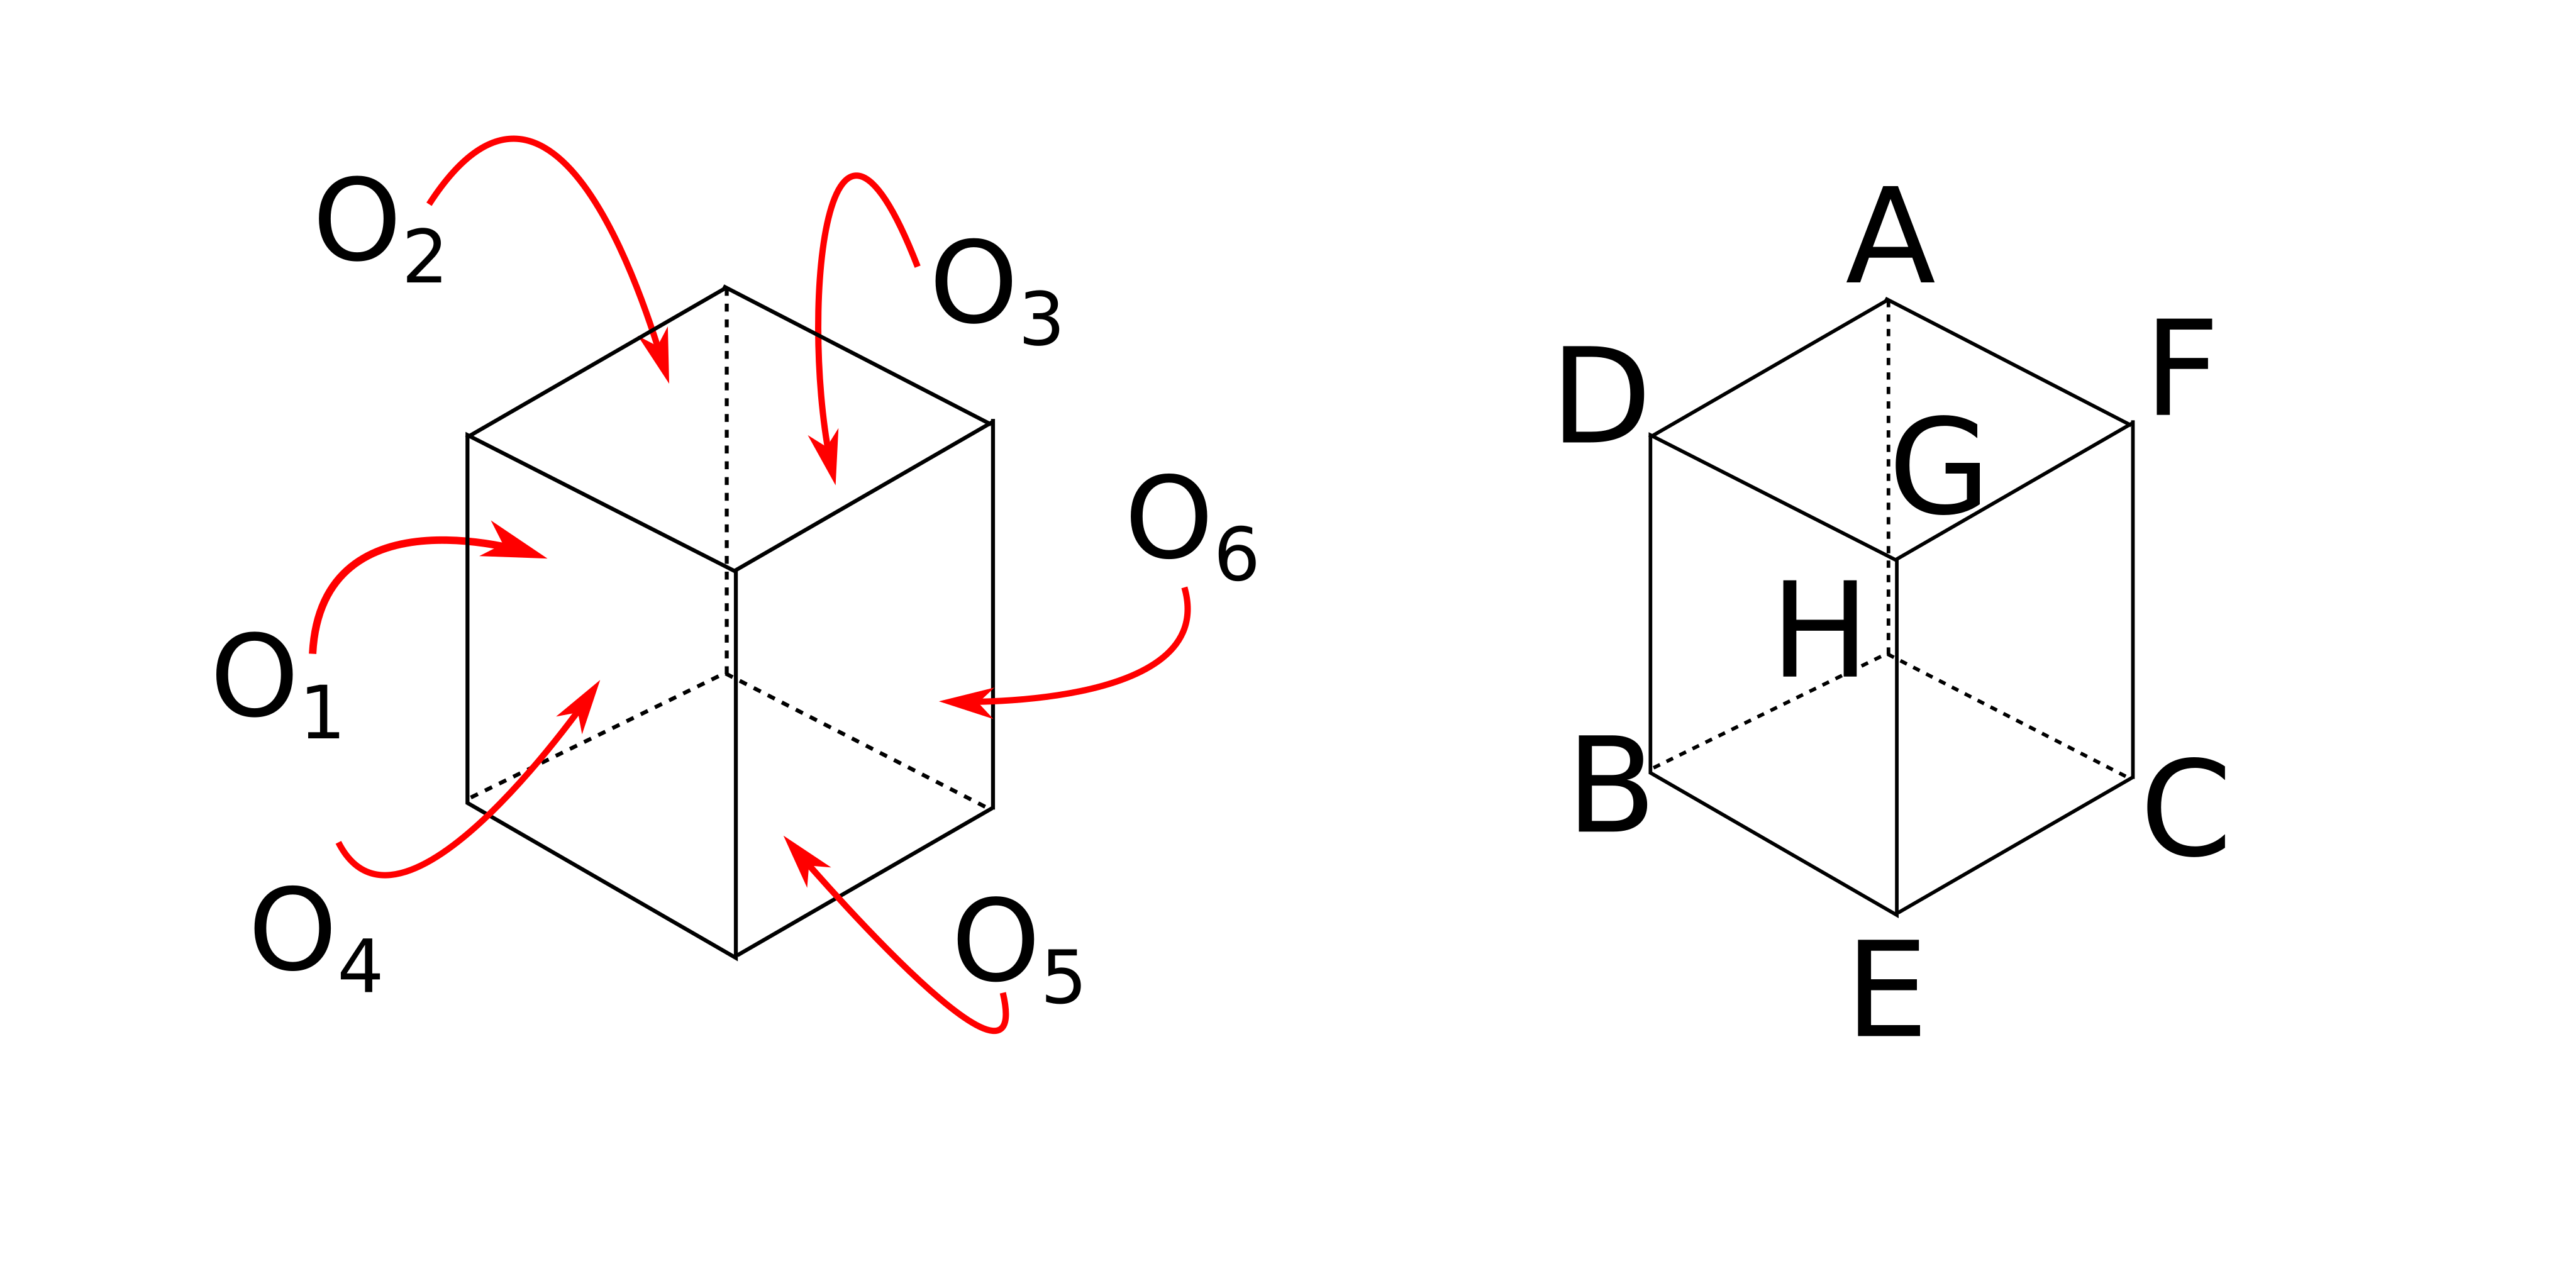
\includegraphics[width=3.5in,
 keepaspectratio]{./img/HexahedraWithSphericalFaces/cubes.png}
 \caption{}
 \label{fig:cubes}
\end{figure}

\begin{figure}[h!tbp]
 \begin{minipage}[t]{0.5\textwidth}
 \centering
 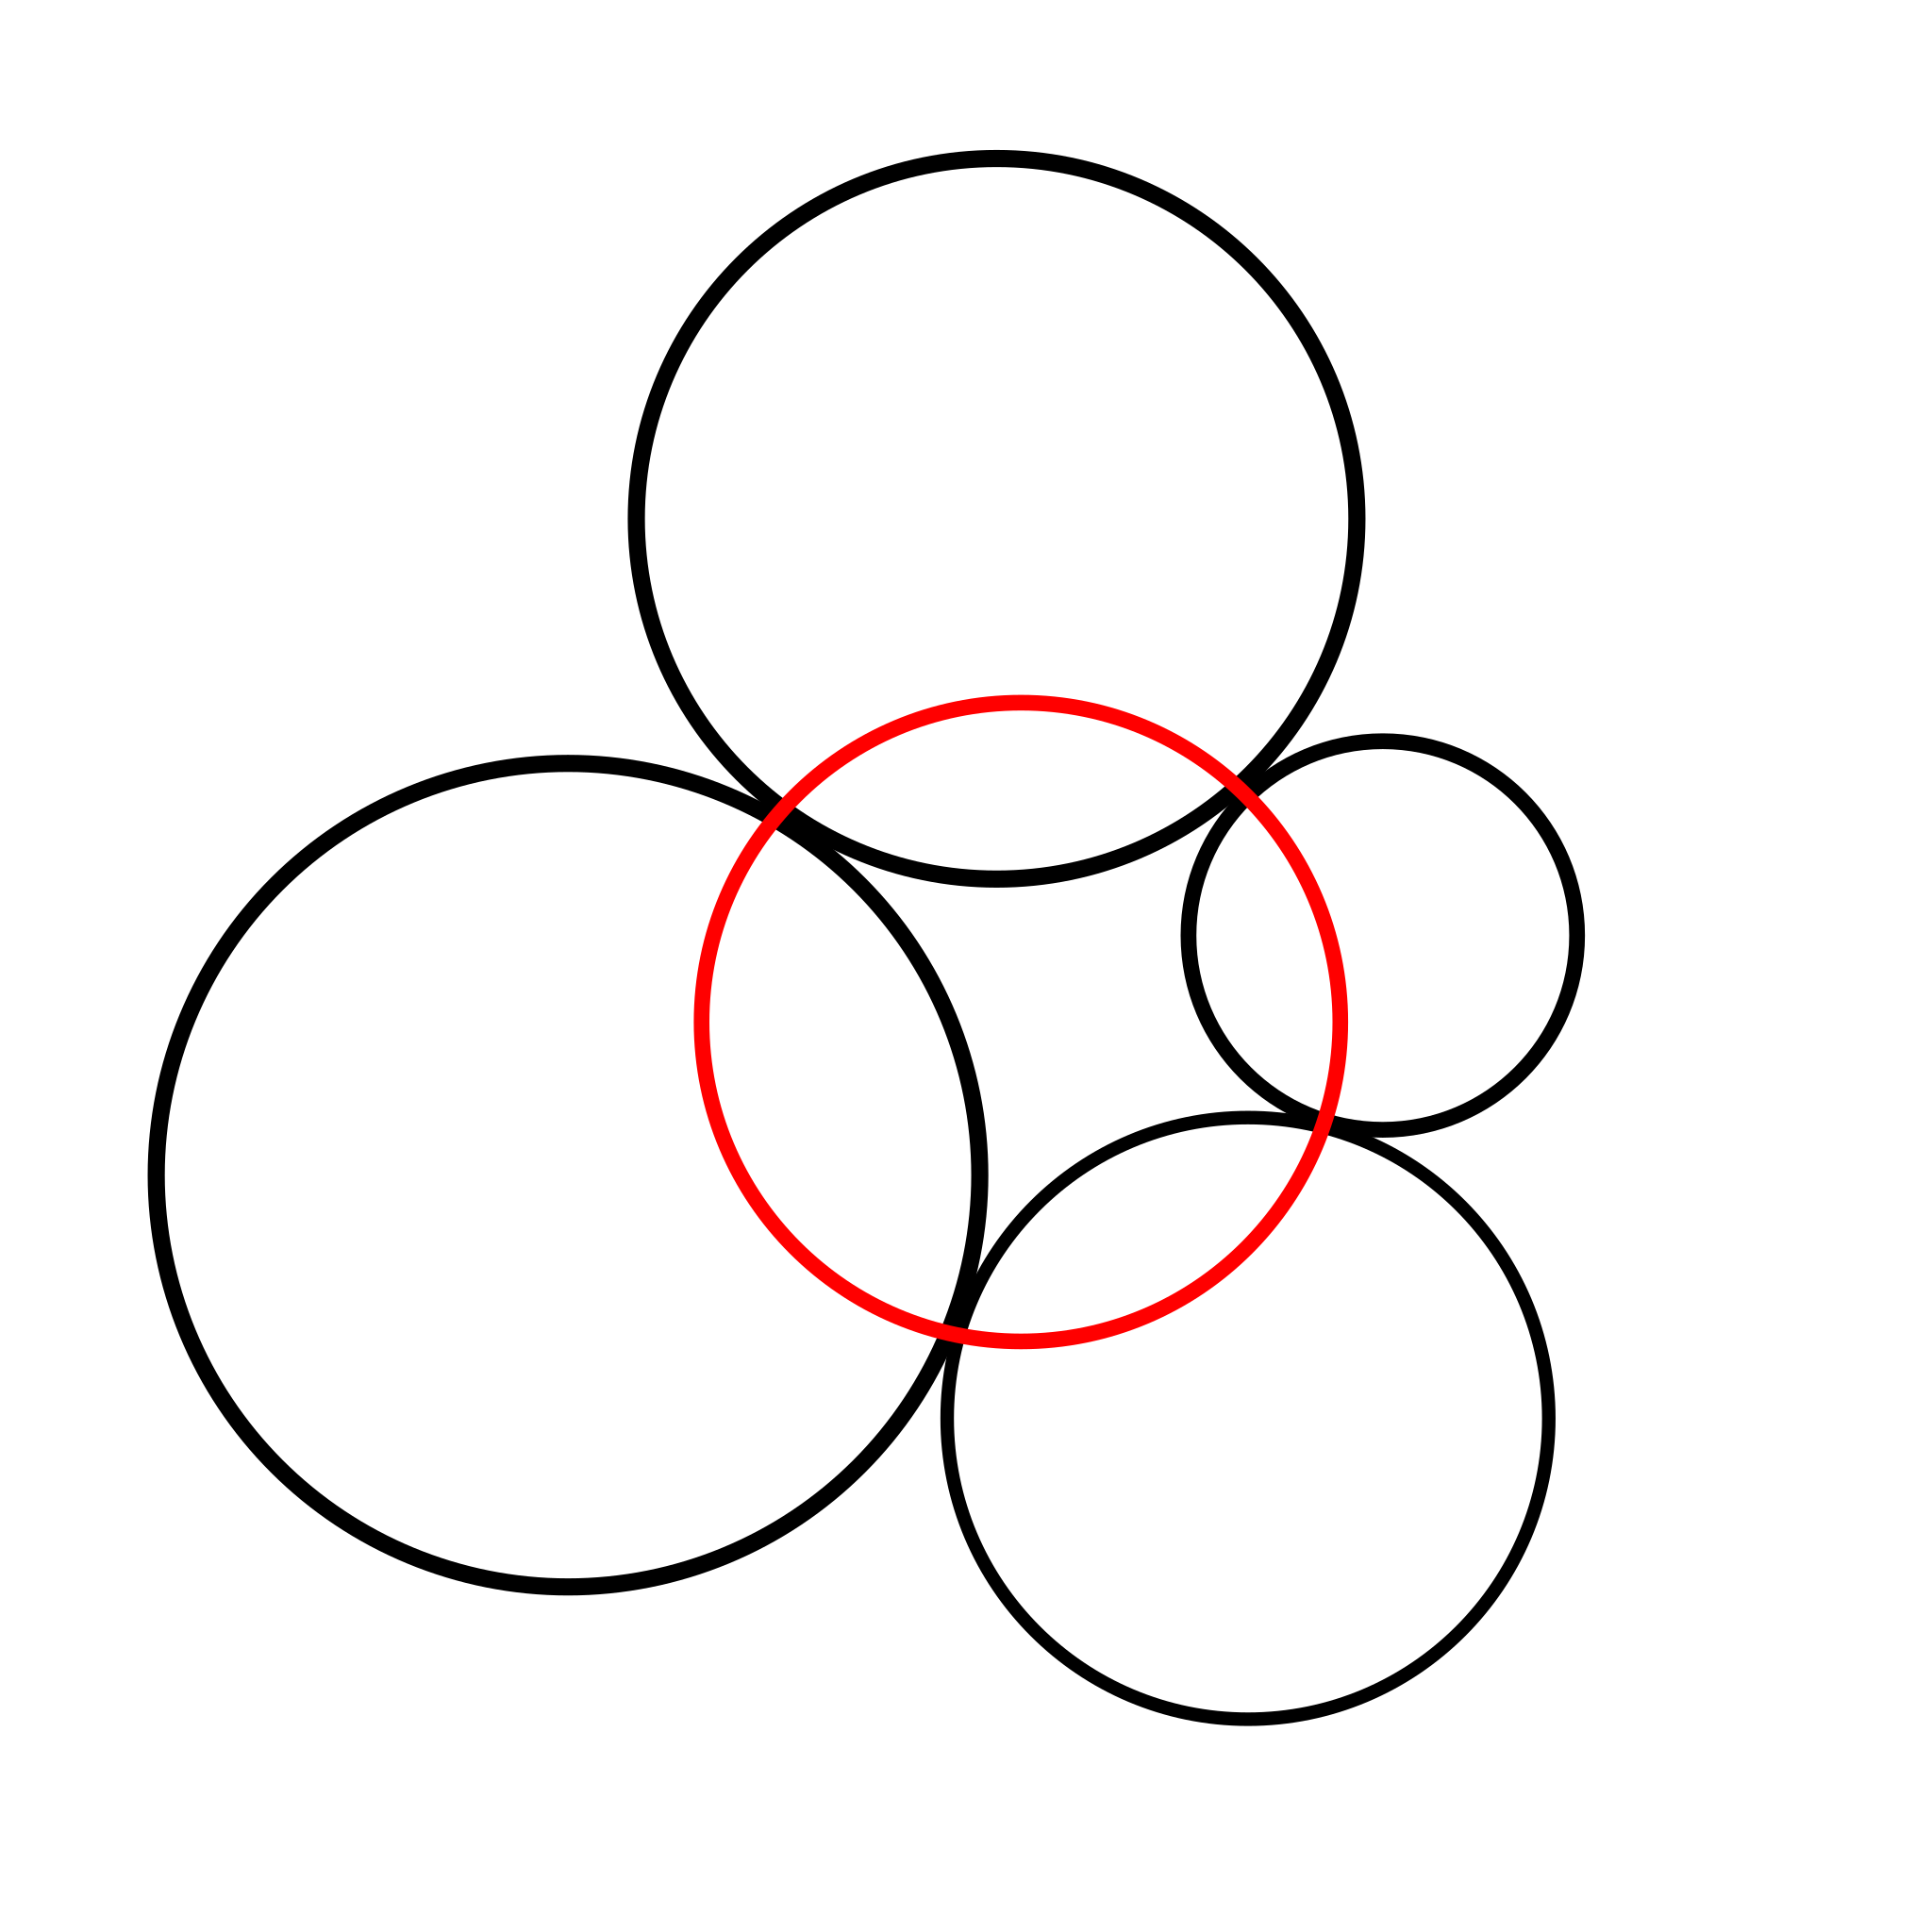
\includegraphics[width=1.5in, height=1.5in,
 keepaspectratio]{./img/HexahedraWithSphericalFaces/chain.png}
 \caption{}
 \label{fig:chainCircles}
 \end{minipage}
 \hspace*{\fill}
 \begin{minipage}[t]{0.5\textwidth}
  \centering
  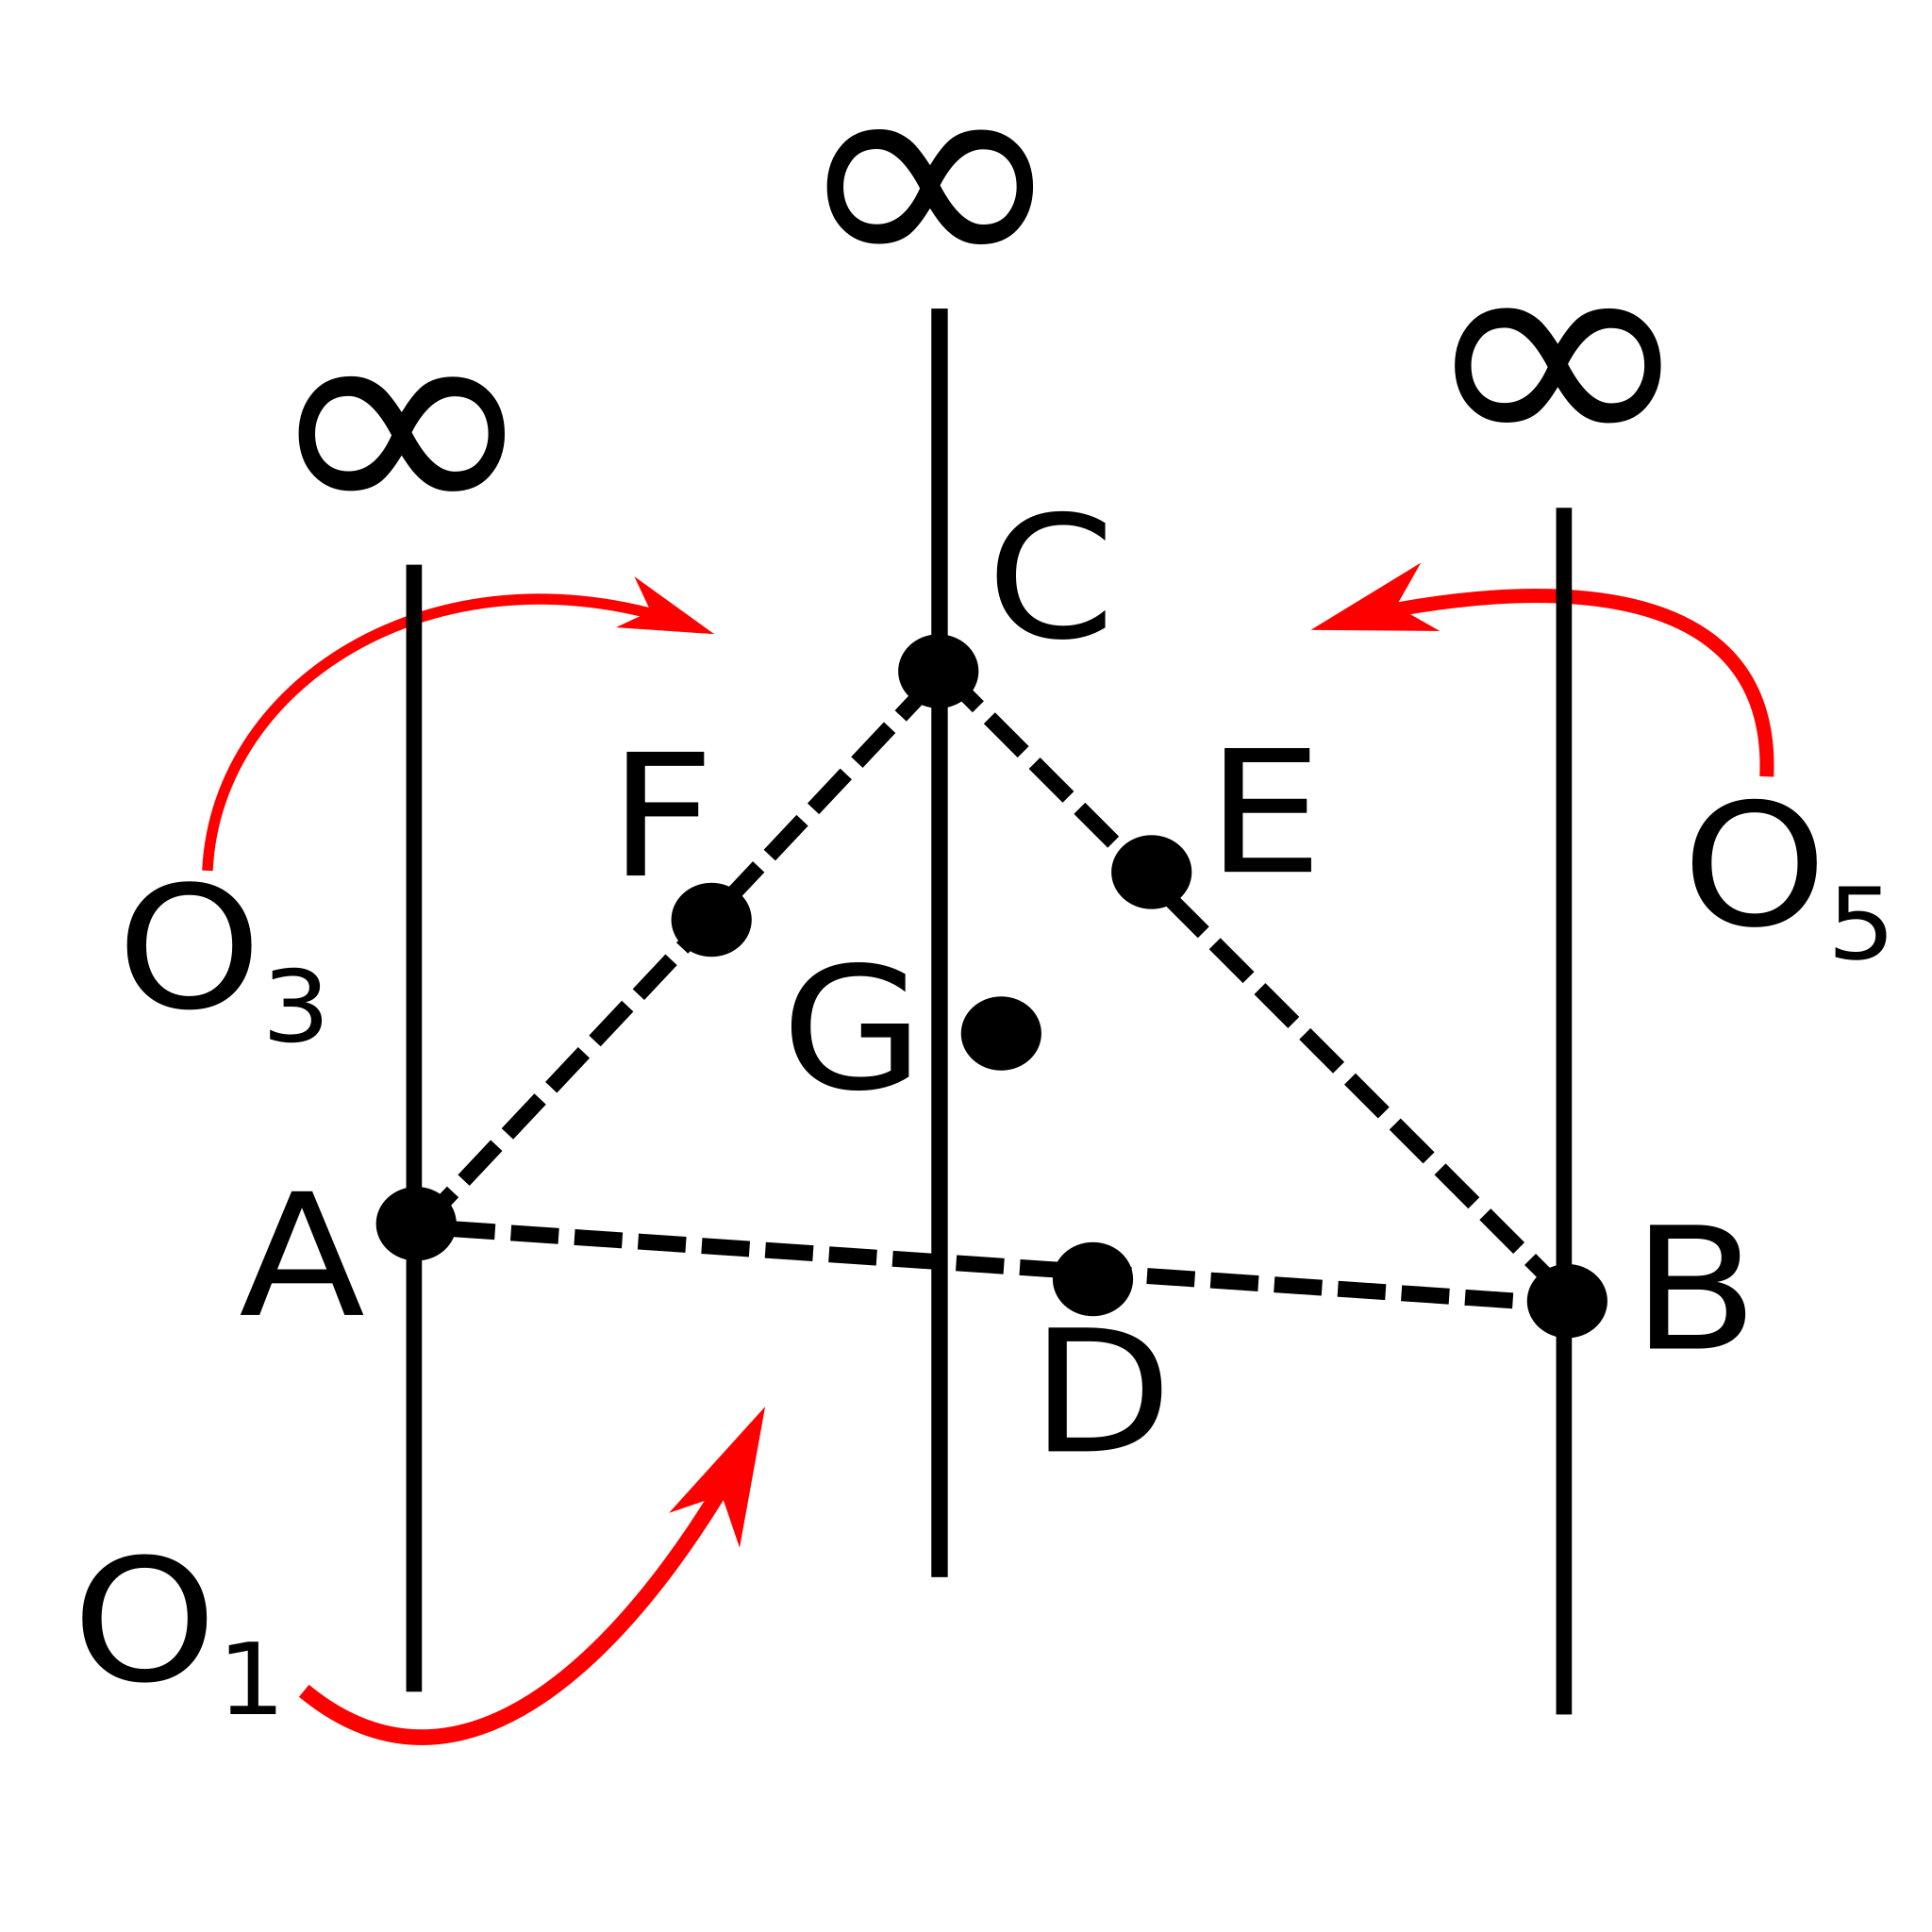
\includegraphics[width=1.5in, height=1.5in,
  keepaspectratio]{./img/HexahedraWithSphericalFaces/infTriangle.png}
  \caption{}
  \label{fig:infTriangle}
 \end{minipage}
 \hspace*{\fill}
\end{figure}

\subsection{Preparations}

We will show sime lemmas in this subsection.

\begin{lemma}\label{sameCircle}
For each $O_i$, the four vertices on $O_i$ lie on the same circle.
Hence the four vertices lie on one plane in $R^3$.
\end{lemma}

\begin{proof}
 We know the following famous lemma about four circles : If four circles 
 $C_1, C_2, C_3, C_4$ on a plane and they are mutually tangent like a
 chain as in Figure \ref{fig:chainCircles}, then the four tangent points lie on one circle.
 (See figure \ref{fig:chainCircles}) Using this lemma we will show lemma \ref{sameCircle} We fix $i$ and
 consider only on $O_i$. If $O_i$ is not a plane, we transform 
 ($O_1, ..., O_6$) by a M\"obius transformation such that $O_i$ is a
 plane. There are four edges on $O_i$ and they are circles and are
 mutually tangent like a chain. From the above well-known lemma. The
 four vertices on $O_i$ lie on one circle on $O_i$. If we re-transform
 ($O_i, ..., O_6$) back, the four vertices still lie on one circle,
 because any M\"obius transformation maps a planer circle to a planer circle.
\end{proof}

\begin{lemma}\label{eightVertices}
 Eight vertices of a polyhedron of cube-type lie on the same sphere.
\end{lemma}

\begin{proof}
 There is a M\"obius transformation $\phi$ such that it moves the vertex
 $H$ to the infinity point. (See Figure \ref{fig:infTriangle}.) From Lemma \ref{sameCircle}, the three
 vertices $A, D,$ and $B$ lie on one straight line. In the same way,
 three vertices $A, D, G,$ and $F$ lie on one planercircle, all vertices
 except $H$ line on one plane. We transform them back by $\phi^{-1}$ and
 we get the conclusion of Lemma \ref{eightVertices}.
\end{proof}

\begin{lemma}\label{sum}
 For each vertex, there are three edges with the vertex. The sum of
 face-angles of these three edges is $\pi$.
\end{lemma}

\begin{proof}
 Let $\phi$ be a M\"obius transformation such that it maps the vertex to
 the infinity point. Then the three edges with the vertex are mapped to
 parallel lines and they form a triangle column. If we consider a
 regular section of the tiangle column then the angles of the section
 are equal to face-angles, and the sum of them is $\pi$ clearly. This
 completes the proof.
\end{proof}

 Using this Lemma \ref{sum}, we obtain the following lemma in a combinatorical way.

\begin{lemma}\label{combination}
 12-ple($n_{ij}$) = ($n_{12}, n_{13}, n_{14}, n_{15}, n_{23}, n_{24},
 n_{26}, n_{35}, n_{36}, n_{45}, n_{46}, n_{56}$) of face-angle
 parameters is one of the following 11.(See Figire 4.)
\end{lemma}

\noindent
(a) (3, 3, 3, 3, 3, 3, 3 ,3 ,3 ,3 ,3 ,3)\\
(b) (2, 3, 3, 3, 6, 6, 2, 3, 3, 3, 3, 3)\\
(c) (2, 3, 6, 3, 6, 3, 2, 3, 3, 2, 6, 3)\\
(d) (6, 2, 3, 3, 3, 2, 3, 6, 3, 3, 6, 2)\\
(e) (3, 2, 2, 3, 6, 6, 2, 6, 3, 6, 3, 2)\\
(f) (3, 2, 2, 3, 6, 6, 3, 6, 2, 6, 2, 3)\\
(g) (6, 2, 2, 3, 3, 3, 6, 5, 2, 6, 2, 3)\\
(h) (3, 2, 6, 3, 6, 2, 3, 6, 2, 2, 6, 3)\\
(i) (4, 2, 2, 4, 4, 4, 2, 4, 4, 4, 4, 2)\\
(j) (4, 2, 2, 4, 4, 4, 4, 4, 2, 4, 2, 4)\\
(k) (6, 2, 2, 4, 3, 3, 6, 4, 2, 4, 2, 4)\\

\begin{figure}[h!tbp]
  \begin{minipage}[t]{0.15\textwidth}
   \centering
   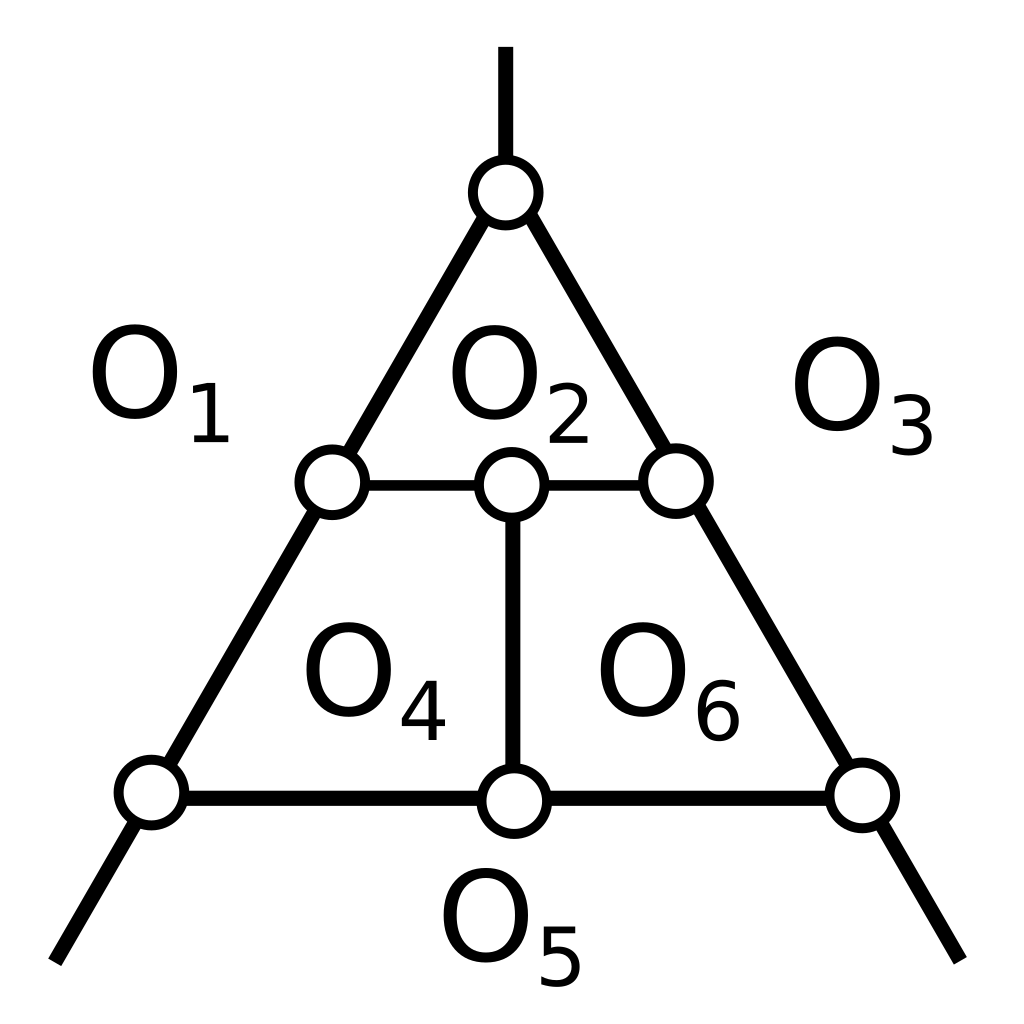
\includegraphics[width=0.8in, keepaspectratio]{./img/HexahedraWithSphericalFaces/cube/cubeFaces.png}
   \subcaption{}
   \label{fig:}
  \end{minipage}
 \hspace*{\fill}
  \begin{minipage}[t]{0.15\textwidth}
   \centering
   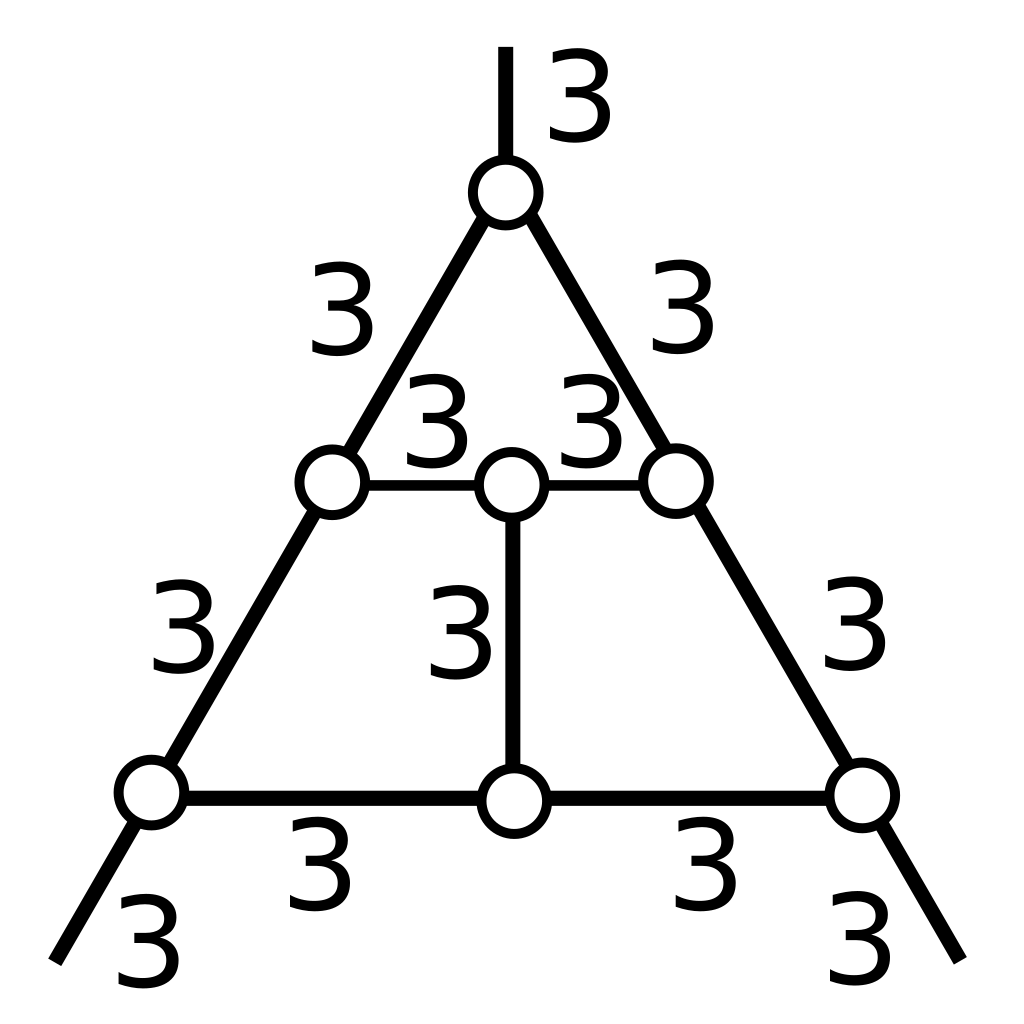
\includegraphics[width=0.8in,
   keepaspectratio]{./img/HexahedraWithSphericalFaces/cube/cube_a.png}
   \subcaption{}
   \label{fig:}
  \end{minipage}
  \hspace*{\fill}
  \begin{minipage}[t]{0.15\textwidth}
   \centering
   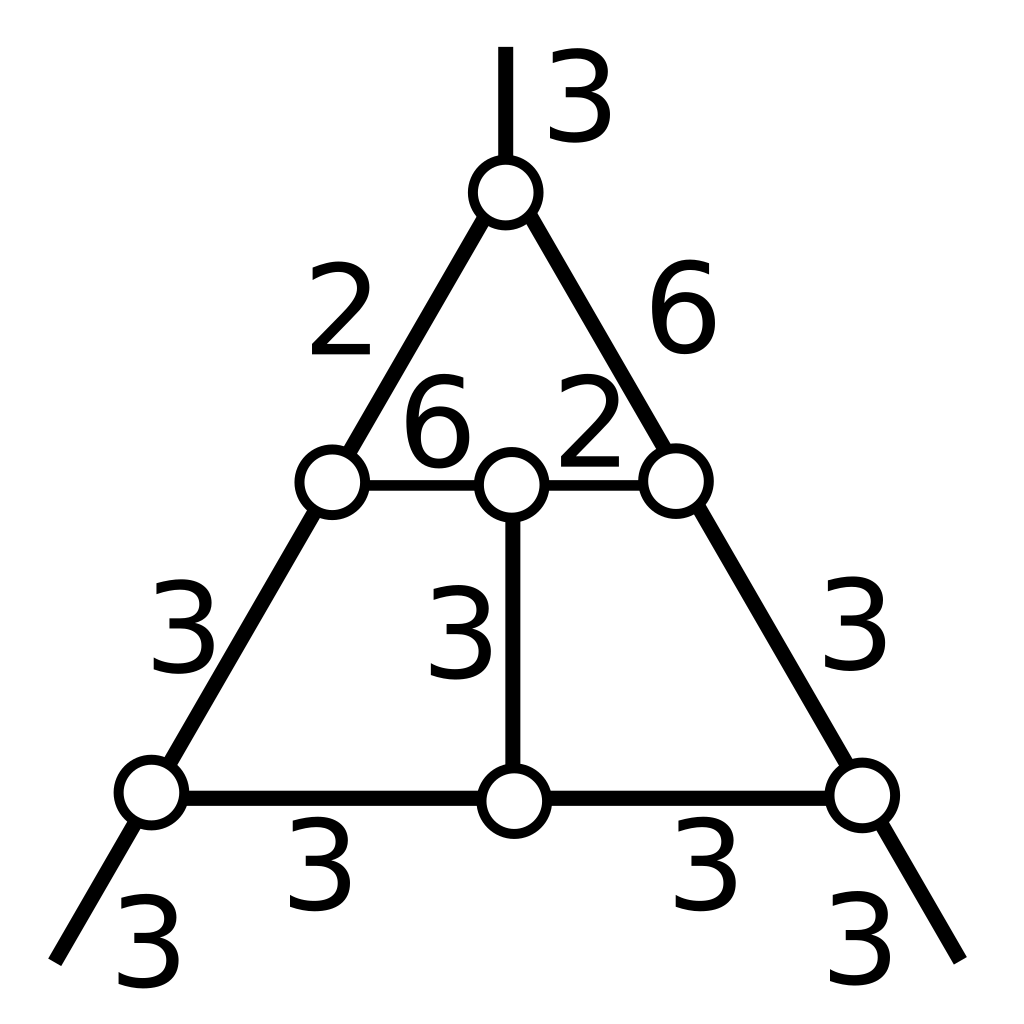
\includegraphics[width=0.8in, keepaspectratio]{./img/HexahedraWithSphericalFaces/cube/cube_b.png}
   \subcaption{}
   \label{}
  \end{minipage}
 \hspace*{\fill}
  \begin{minipage}[t]{0.15\textwidth}
   \centering
   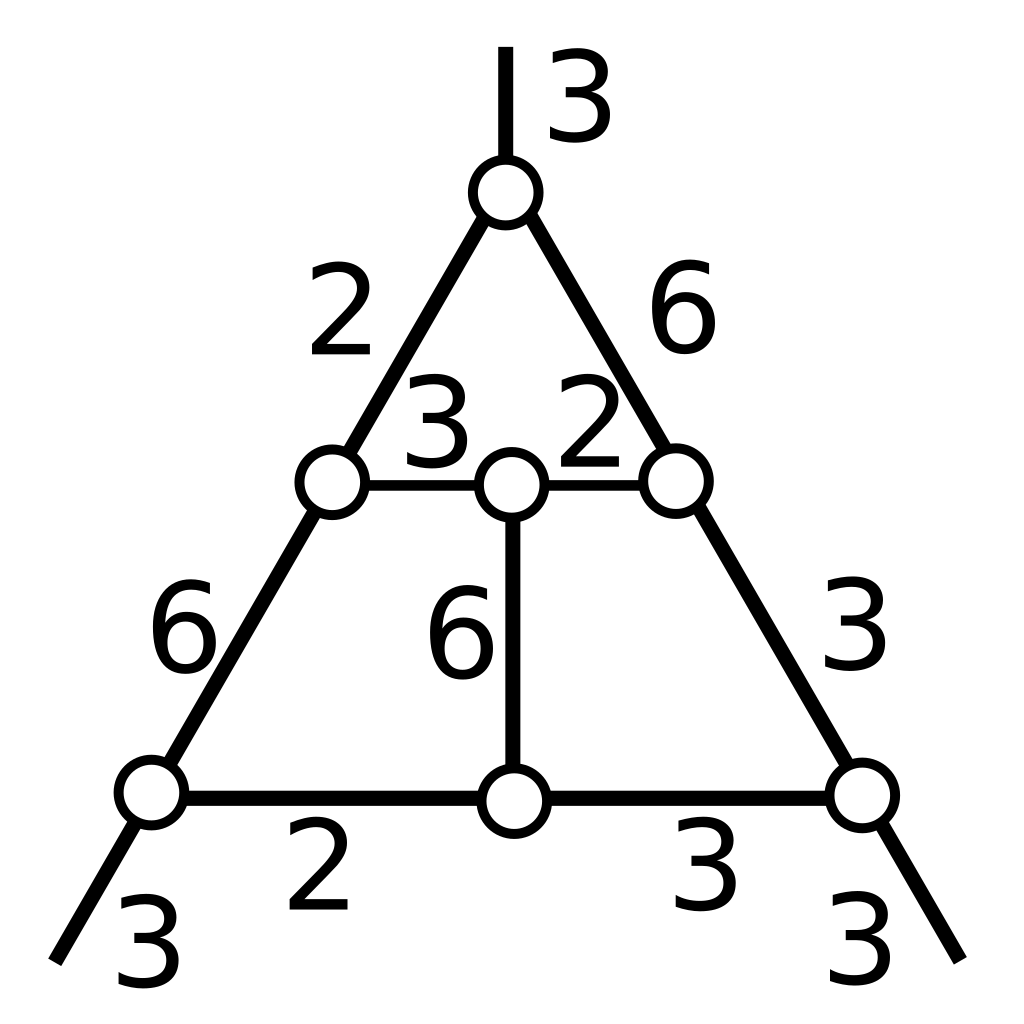
\includegraphics[width=0.8in, keepaspectratio]{./img/HexahedraWithSphericalFaces/cube/cube_c.png}
   \subcaption{}
   \label{fig:}
  \end{minipage}
 \hspace*{\fill}
  \begin{minipage}[t]{0.15\textwidth}
   \centering
   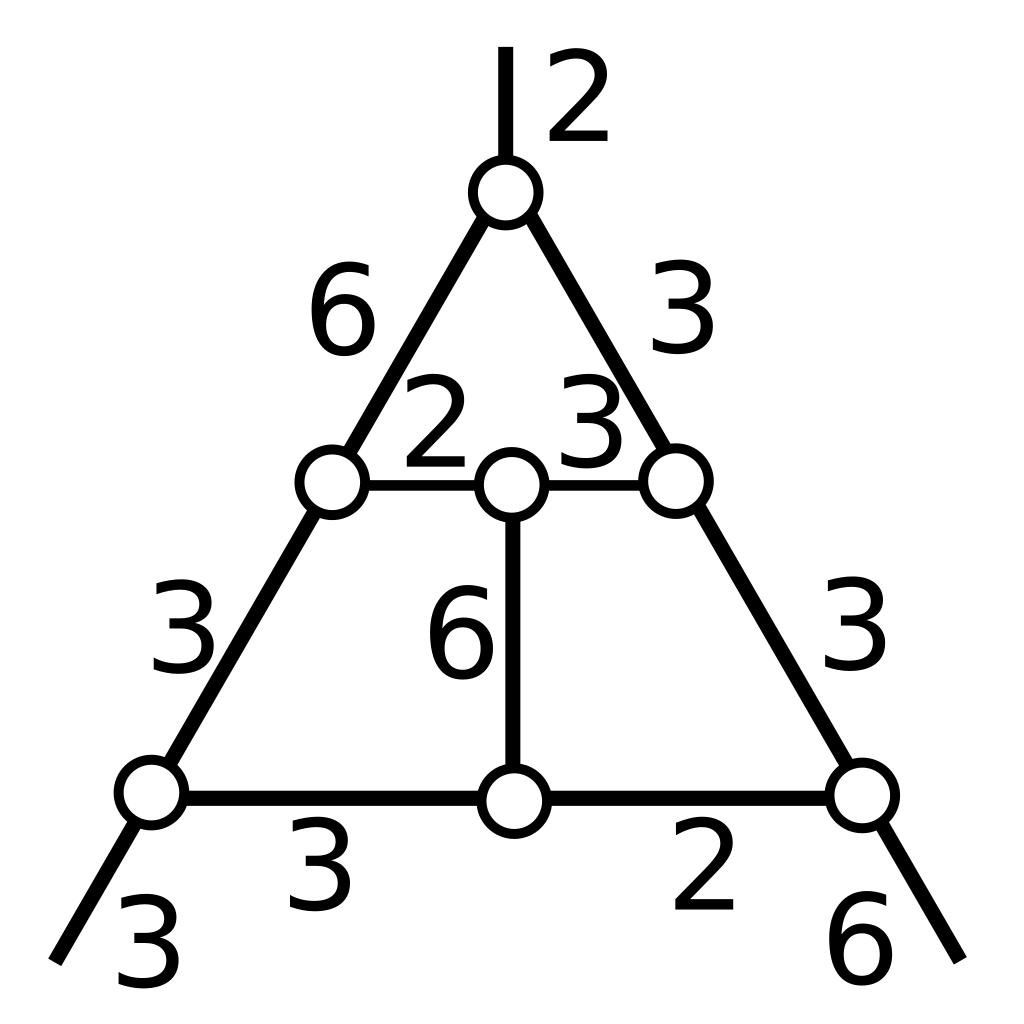
\includegraphics[width=0.8in, keepaspectratio]{./img/HexahedraWithSphericalFaces/cube/cube_d.png}
   \subcaption{}
   \label{fig:}
  \end{minipage}
 \hspace*{\fill}
  \begin{minipage}[t]{0.15\textwidth}
   \centering
   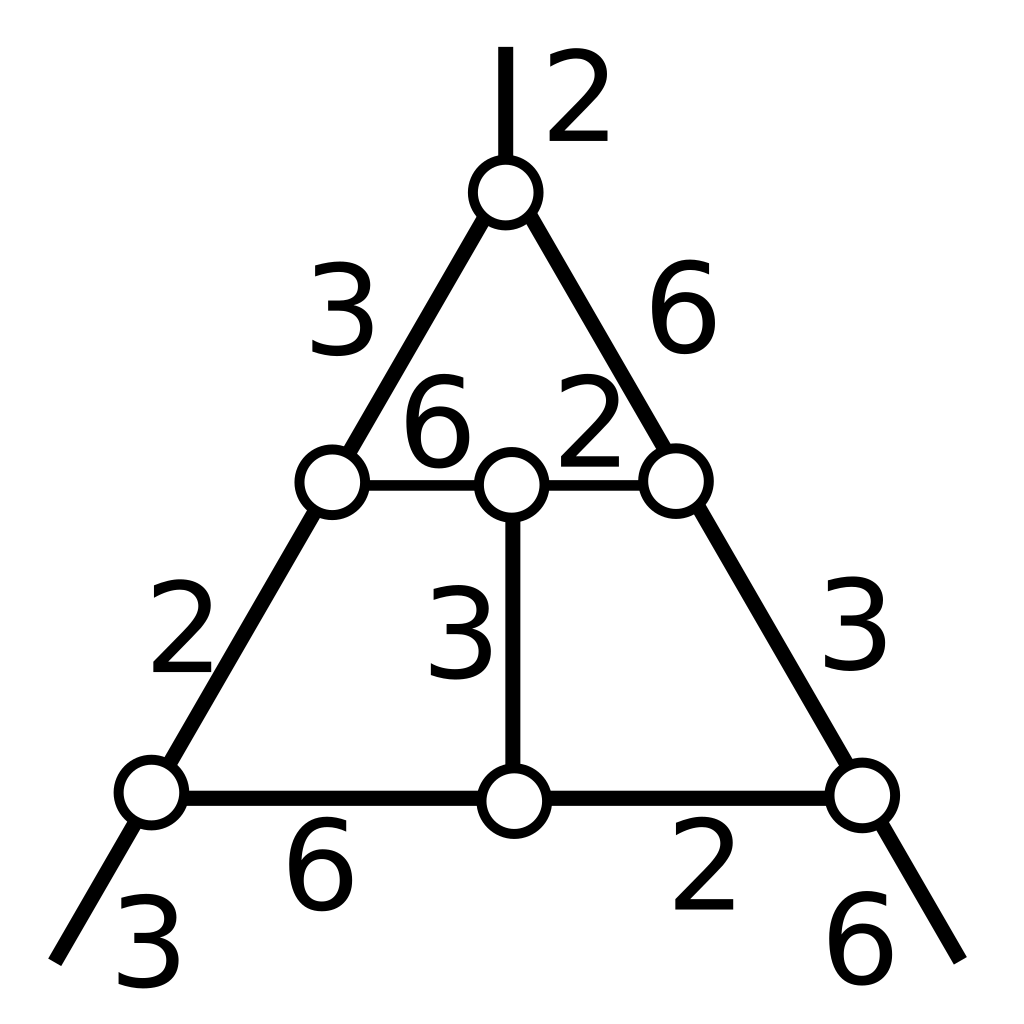
\includegraphics[width=0.8in, keepaspectratio]{./img/HexahedraWithSphericalFaces/cube/cube_e.png}
   \subcaption{}
   \label{fig:}
  \end{minipage}
 \hspace*{\fill}
\begin{minipage}[t]{0.15\textwidth}
   \centering
   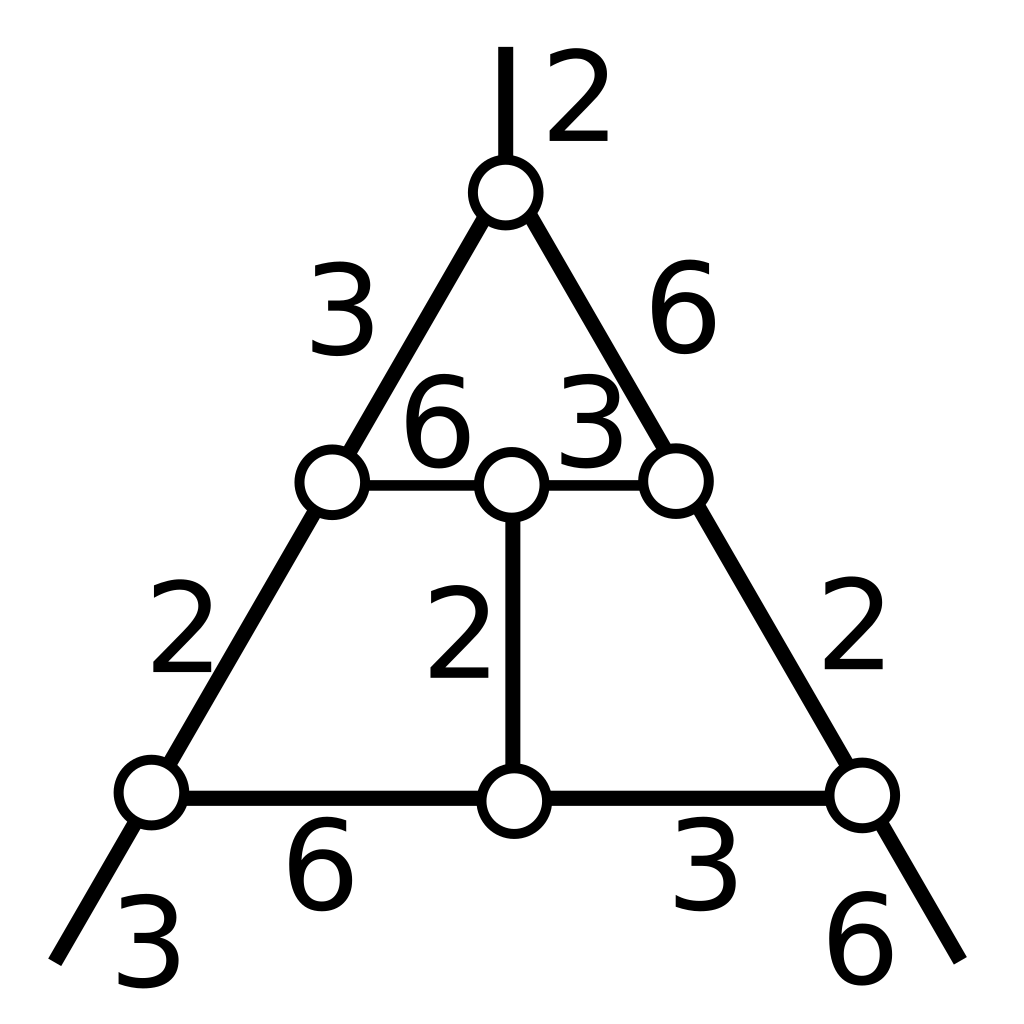
\includegraphics[width=0.8in,
 keepaspectratio]{./img/HexahedraWithSphericalFaces/cube/cube_f.png}
   \subcaption{}
   \label{fig:}
  \end{minipage}
 \hspace*{\fill}
  \begin{minipage}[t]{0.15\textwidth}
   \centering
   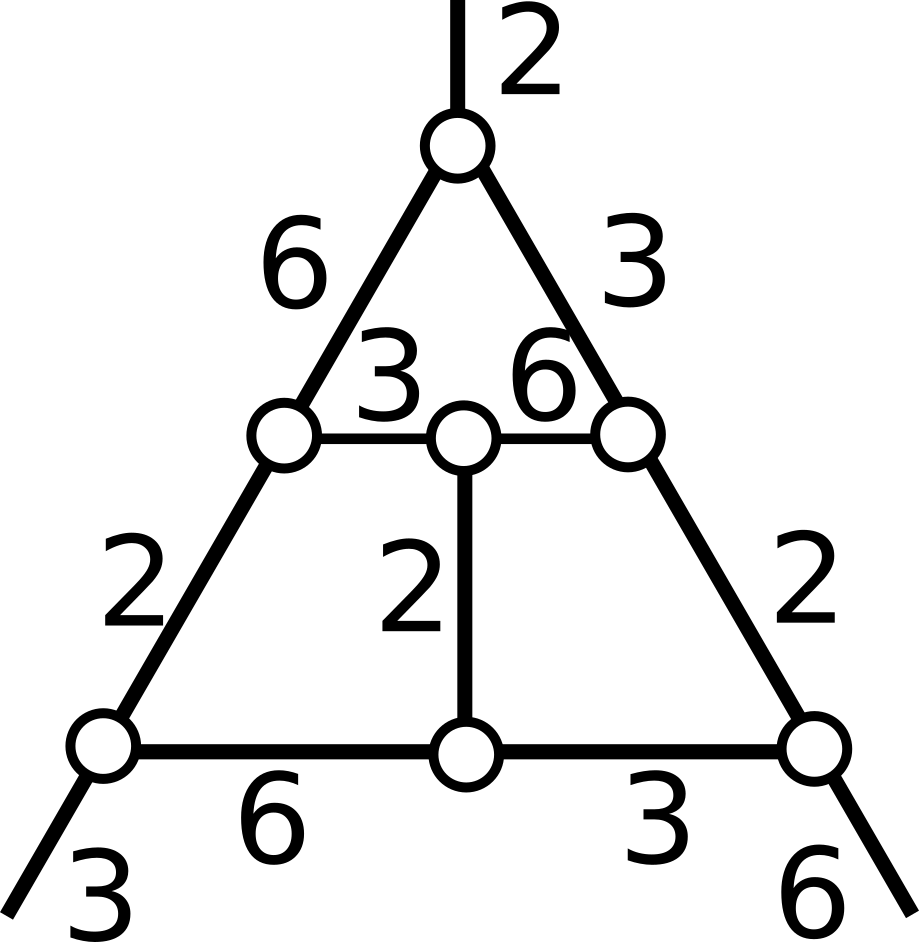
\includegraphics[width=0.8in,
   keepaspectratio]{./img/HexahedraWithSphericalFaces/cube/cube_g.png}
   \subcaption{}
   \label{fig:}
  \end{minipage}
  \hspace*{\fill}
  \begin{minipage}[t]{0.15\textwidth}
   \centering
   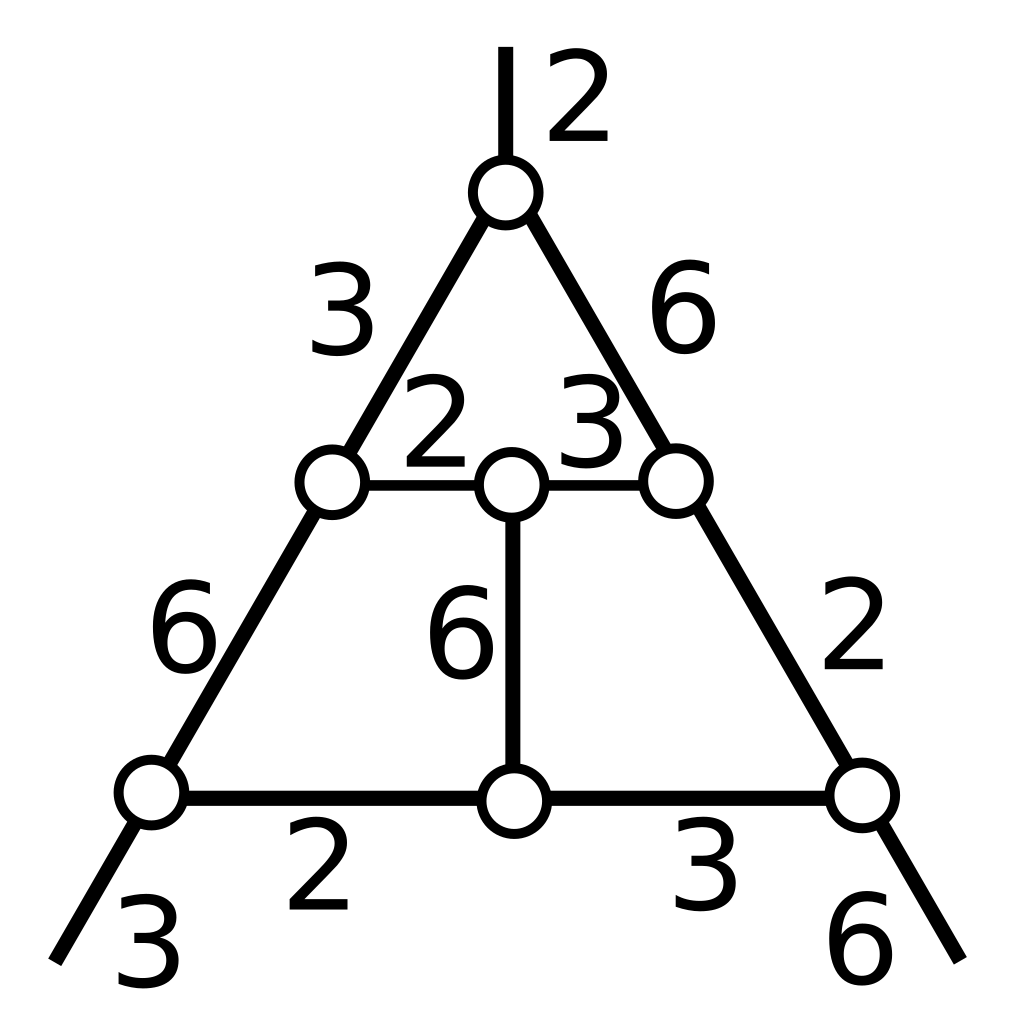
\includegraphics[width=0.8in, keepaspectratio]{./img/HexahedraWithSphericalFaces/cube/cube_h.png}
   \subcaption{}
   \label{}
  \end{minipage}
 \hspace*{\fill}
  \begin{minipage}[t]{0.15\textwidth}
   \centering
   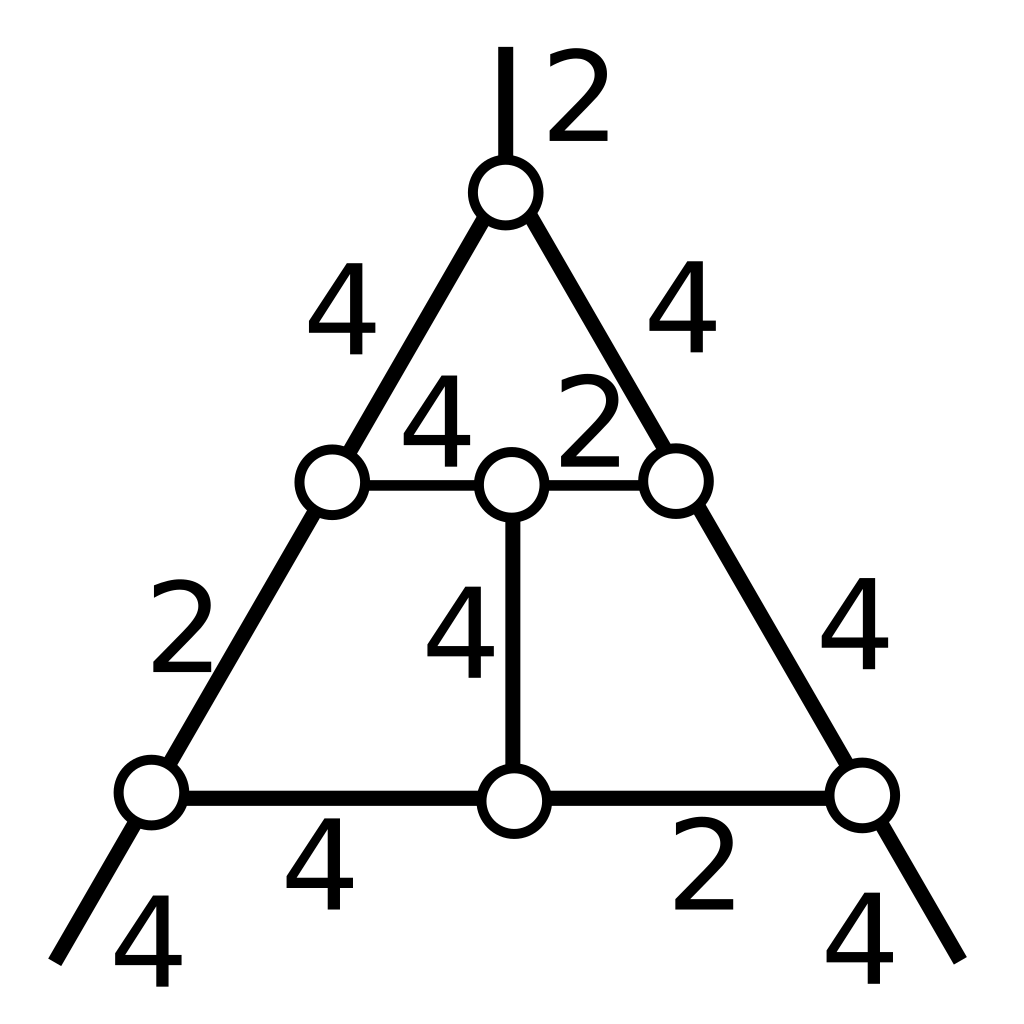
\includegraphics[width=0.8in, keepaspectratio]{./img/HexahedraWithSphericalFaces/cube/cube_i.png}
   \subcaption{}
   \label{fig:}
  \end{minipage}
 \hspace*{\fill}
  \begin{minipage}[t]{0.15\textwidth}
   \centering
   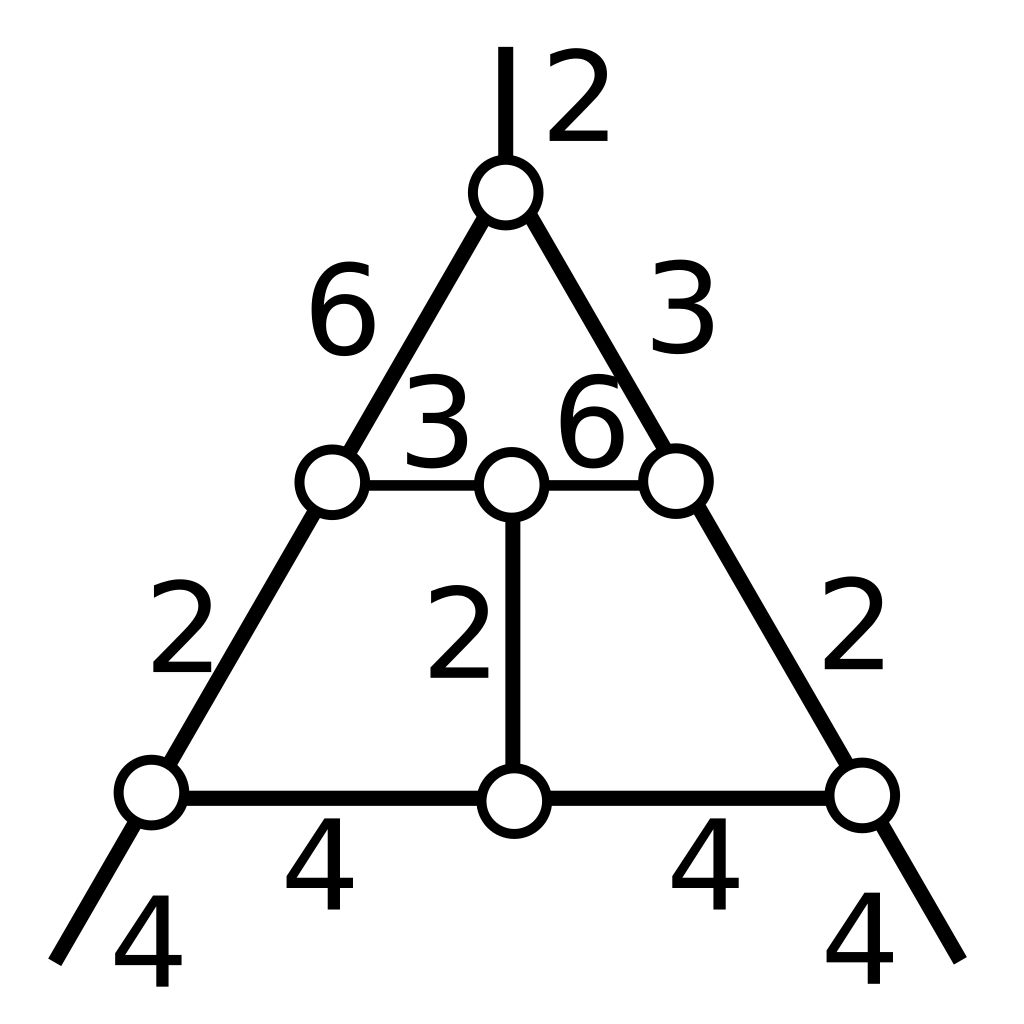
\includegraphics[width=0.8in, keepaspectratio]{./img/HexahedraWithSphericalFaces/cube/cube_j.png}
   \subcaption{}
   \label{fig:}
  \end{minipage}
 \hspace*{\fill}
  \begin{minipage}[t]{0.15\textwidth}
   \centering
   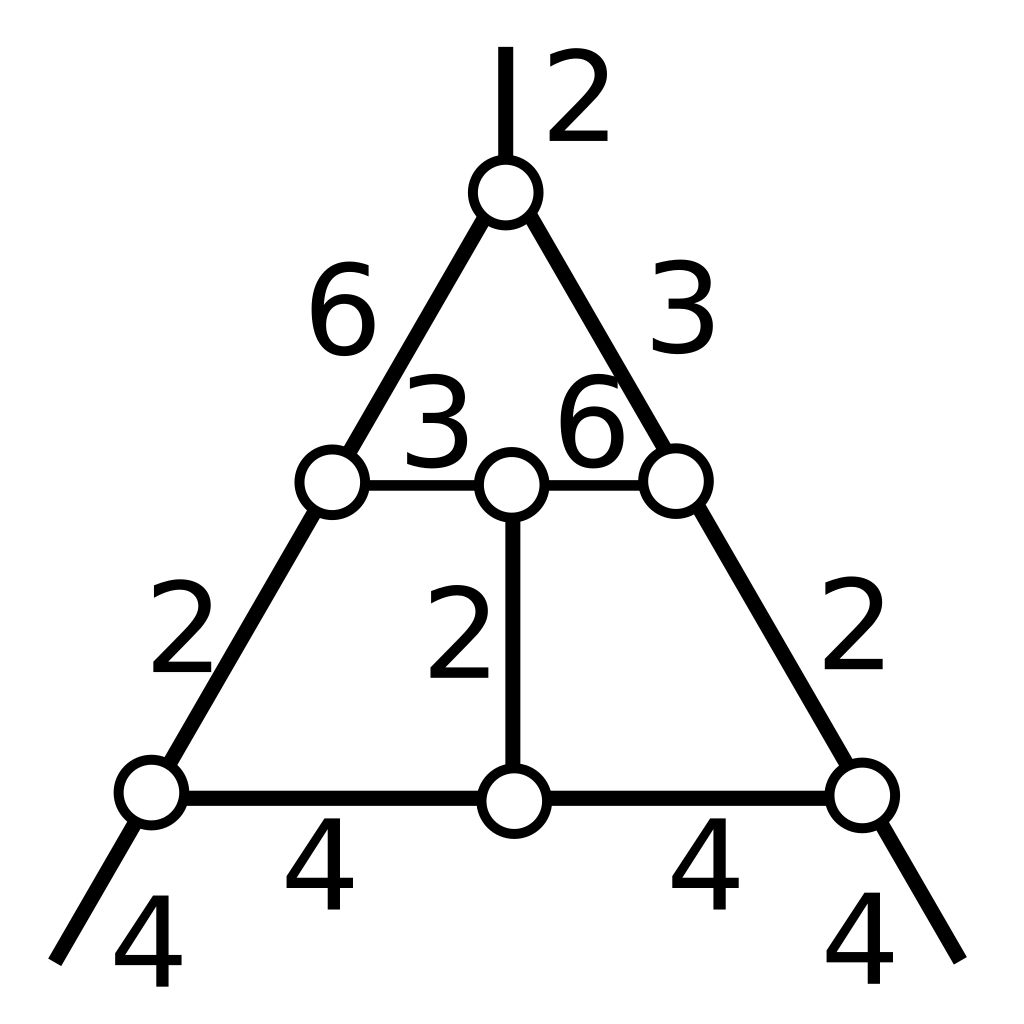
\includegraphics[width=0.8in, keepaspectratio]{./img/HexahedraWithSphericalFaces/cube/cube_k.png}
   \subcaption{} % TODO k is same to j
   \label{fig:}
  \end{minipage}
 \hspace*{\fill}
  \caption{\textit{Full-colored printing by DMM.make 3D print.}}
  \label{fig:}
\end{figure}

We get this lemma only in combinatorical way, so we omit the proof.

In order to represent a sphairahedron, we use a polyhedral graph as
shown in Figure []. The graph shows an infinite cube-type sphairahedron.
The black lines represent edges, and the circles represent
vertices. The three radial edges connect the infinite vertex and finite
vertices. Each of the numbers beside 
the edges means a natural number $n$ for the dihedral angle $\pi / n$

In this preview section we introduce that there are 7 types of
combination of face angles. But here are 11. In fact, in case (f), (g),
(j), and (k), there is no polyhedron with these face-angles. See section 2.6.

\subsection{Constructing hexahedron}

We fix a set($n_{ij}$) of face-angles and consider conformal equivalent
classes of polyhedra with (P1), (P2), (P3).

In the sequel we suppose that $H = \infty$. (See Figure \ref{fig:infTriangle}) So the three
edges $HA, HB, HC$ are straight lines and are parallel to each other. We
assume that they are perpendicular to xy-plane.
Let ($x_A, y_B, z_z$), ..., ($x_G, y_G, z_G$) be coordinates of vertices
A, B, ..., G (except $H$) respectively. Let $A'(x_A, y_A)$, ...,$G'(x_G,
y_G)$ be projection of these 7 vertices to the xy-plane.

We get immediately that $\angle C'A'B' = \theta_{13}, \angle A'B'C' =
\theta_{15}, \angle B'C'A'=\theta_{13}$. Remark that $\theta_{13} +
\theta_{15} + \theta_{35} = \pi$ by Lemma\ref{sum}.

Here we may assume that the radius of the circumcircle of $A'B'C'$ is 1,
that the circumcenter of $A'B'C'$ is $(0, 0, 0)$, and that $A'$ is on
the x-axis. If it is not, by a proper M\"obius transformation(such that
it fixes the infinity point,) and it is easy to let the polyhedron
satisfy these conditions. By parallel transformation along z-axis, we
may assume that $A$ is on xy-plane. (That is, $A = A'$ and $z_A = 0.$)

See Figure \ref{fig:infTriangle} again. $O_2, O_4, O_6$ are spheres Let $O_i(x_i, y_i, z_i)$
and $r_i$ be the center and the radius of $O_i$ for $i = 2, 4, 6.$ About
the radius, we have the following proposition.

\begin{figure}[h!tbp]
 \centering
 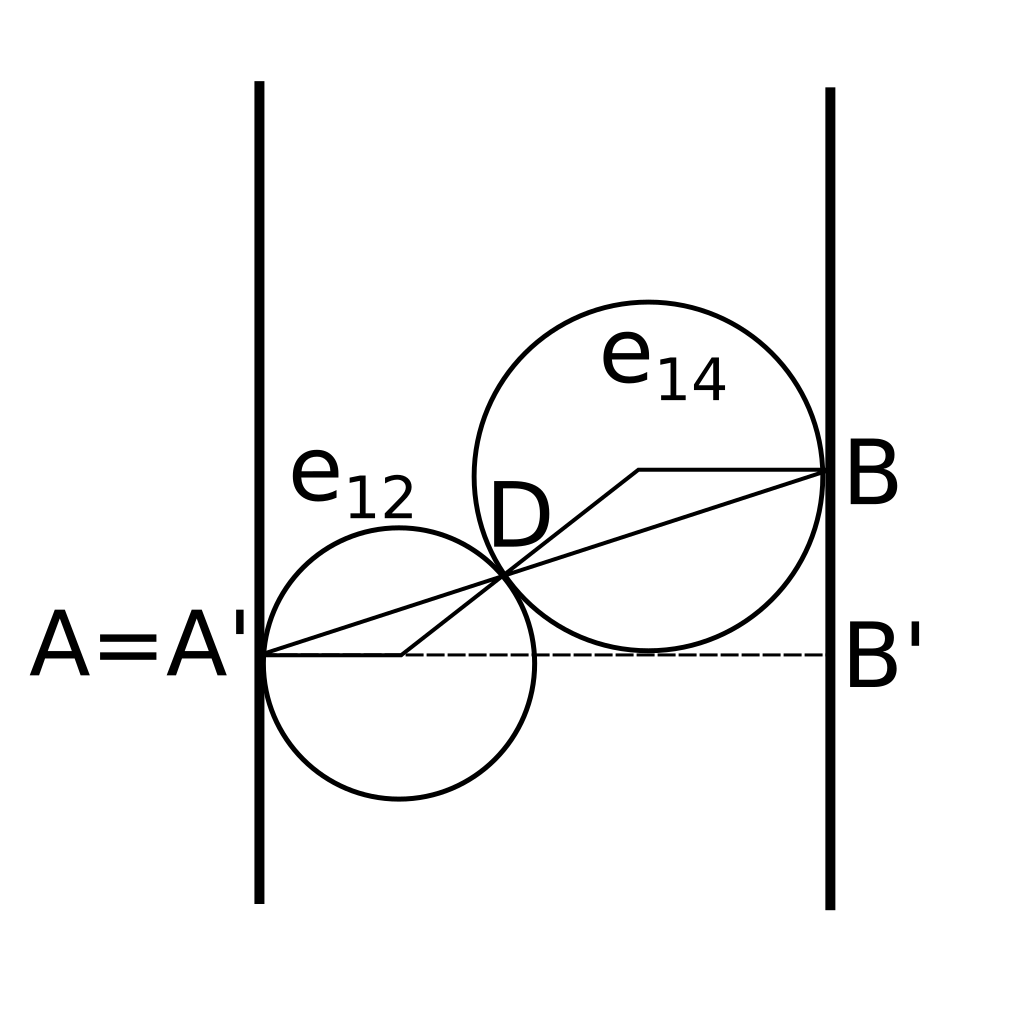
\includegraphics[width=3.5in, height=3.5in,
 keepaspectratio]{./img/HexahedraWithSphericalFaces/sideSlice.png}
 \caption{}
 \label{fig:sideSlice}
\end{figure}

\begin{proposition}\label{angles}
 \begin{eqnarray}
 r_2\sin\theta_{12} + r_4\sin\theta_{14} &=& \overline{AB}^2 / (2\overline{A'B'})\\
 r_4\sin\theta_{45} + r_6\sin\theta_{56} &=& \overline{BC}^2 / (2\overline{B'C'})\\
 r_2\sin\theta_{23} + r_6\sin\theta_{36} &=& \overline{CA}^2 / (2\overline{C'A'})
 \end{eqnarray}
\end{proposition}

\begin{proof}
 In Figure \ref{fig:sideSlice}. the edge $AD = e_{12}$ is a circle with radius
 $r_2\sin\theta_{12}$, and the edge $DB e_{14}$ is a circle with radius
 ($r_4\sin\theta_{14}$).
Two vertical lines $HA$ and $HB$ are tangent to these circles as in
 Figure \ref{fig:sideSlice},
 and we have 
 \begin{eqnarray*}
  \overline{AD} = 2 r_2 \sin\theta_{12} \cdot \overline{A'B'}/\overline{AB}\\
  \overline{DB} = 2 r_4 \sin\theta_{14} \cdot \overline{A'B'}/\overline{AB}
 \end{eqnarray*}
 Remark that $\cos(\angle BAB') =\overline{A'B'}/\overline{AB}.$ Clearly
 $\overline{AD} + \overline{DB} = \overline{AB}$ holds, so it is easy to
 show the first formula of Proposition \ref{angles}. Others are shown in the same
 way.

\end{proof}

\begin{remark}
 If we regard ($2.A$) as linear equation on $r_2, r_4, r_6$, the
 coordinate matrix of ($2.A$) is not singular. In fact,
 \begin{eqnarray*}
  \left| 
   \begin{array}{ccc}
    \sin\theta_{12} & \sin\theta_{14} & 0\\
    0               & \sin\theta_{45} & \sin\theta_{56}\\
    \sin\theta_{32} & 0               & \sin\theta_{36}
   \end{array}
  \right|
 \end{eqnarray*}
 is positive.
 If we fix three vertices $A, B, C$ then always there are solutions of
 (2.A), but they may be non-positive. And, if $r_2$ or $r_4$ or $r_6$
 are too large, ($O_i$) doesn't form a hexahedron. For example, see
 subsection \ref{extend}. In this section, we know that $r_2, r_4, r_6$ are all
 'valid' if and only if parameters ($z_B, z_C$) are in the restricted are
 area

Next, we will obtain the coordinate of the centers of $O_2, O_4, O_6$.
Let $O_i'(x_i, y_i)$ be a projection of the center of the sphere $O_i$
 to xy-plane (for i = 2, 4, 6.)
\end{remark}

\begin{figure}[h!tbp]
 \centering
 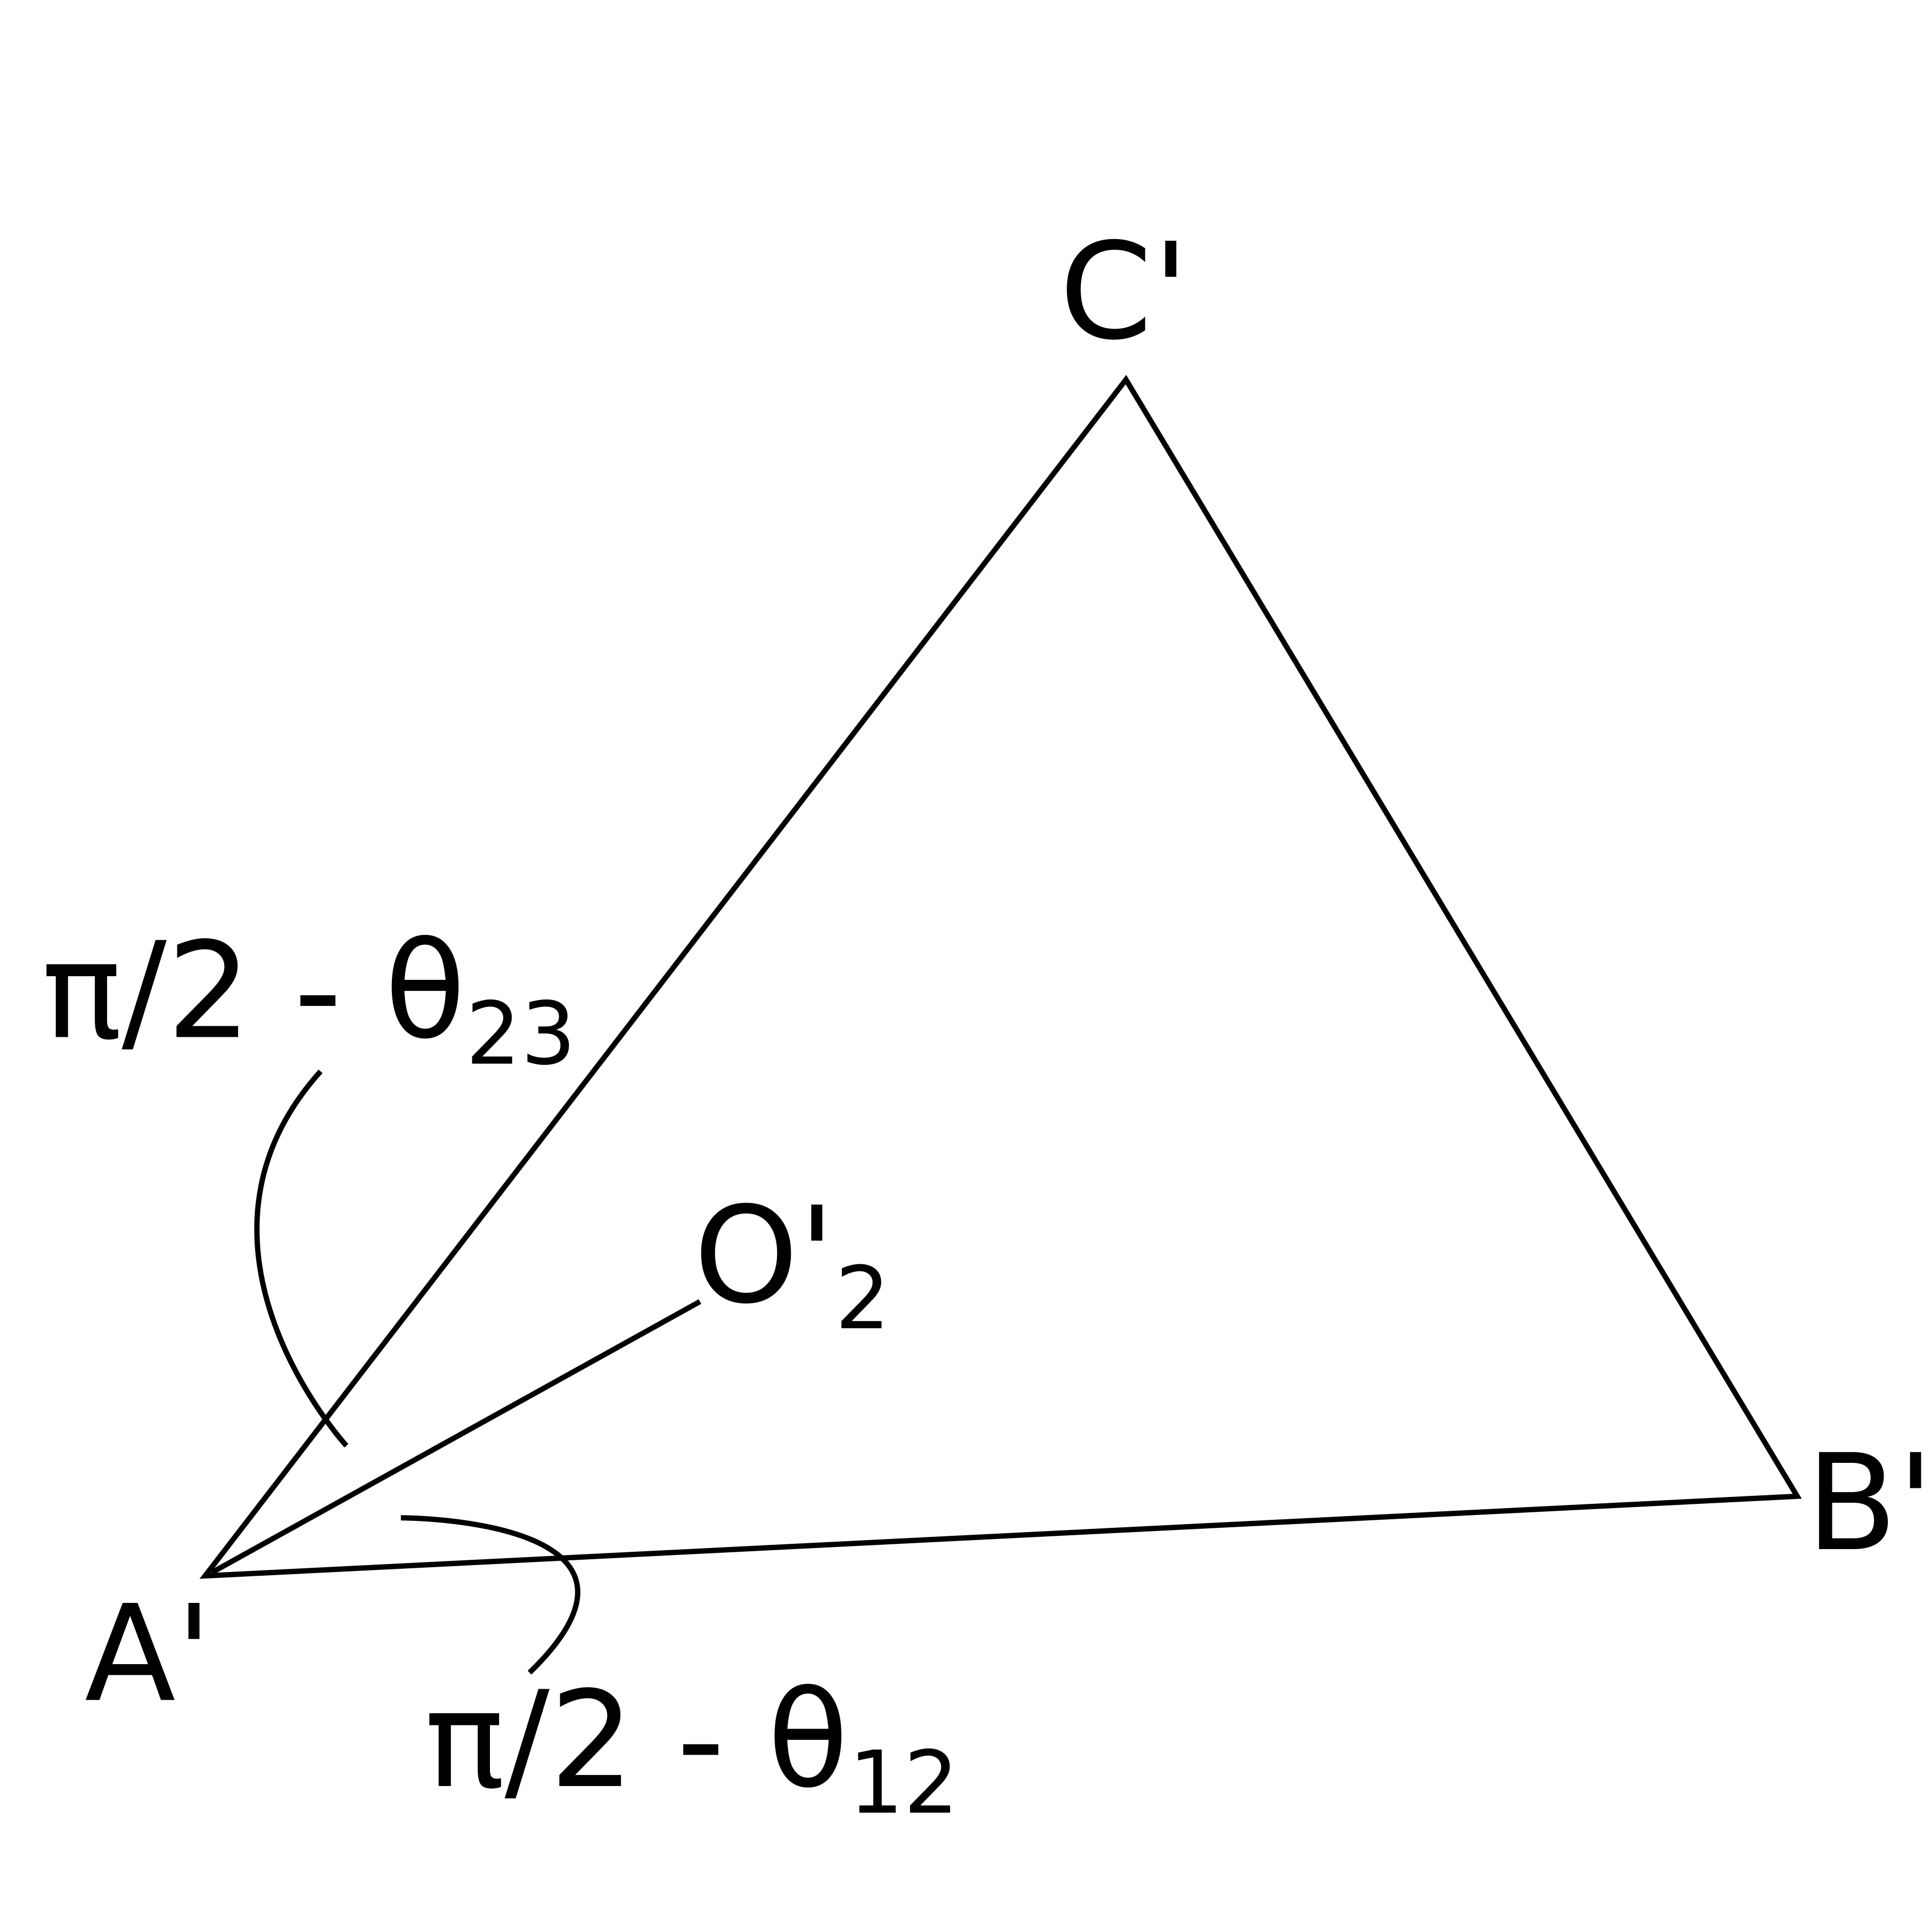
\includegraphics[width=3.5in, height=3.5in,
 keepaspectratio]{./img/HexahedraWithSphericalFaces/abcTriangle.png}
 \caption{}
 \label{fig:sideSlice}
\end{figure}

\begin{proposition}\label{angles}
 (1)$\angle O_2'A'B' = \pi/2 - \theta_{12}, \angle
 O'_2A'C'=\pi/2-\theta_{23}$.

  $\angle O_4'B'A' = \pi/2 - \theta_{14}, \angle O_4'B'C' = \pi/2 -
 \theta_{45}$.

 $\angle O_6'C'A' = \pi/2 - \theta_{36}, \angle O_6'C'A' = \pi/2 - \theta_{56}$.

 (2)$z_A = z_2 = 0$ and $\overline{A'O'_2} = \overline{AO_2} = r_2$

 $z_B = z_4$ and $\overline{B'O'_4} = \overline{BO_4} = r_4$

 $z_C = z_6$ and $\overline{C'O'_6} = \overline{CO_6} = r_6$
\end{proposition}

\begin{proof}
 (1) Since the face-angle of the plane $O_1$ and the sphere $O_2$ is
 $\theta_{12}$, the angle of a straight line $A'B'$ and a circle with
 center $O'_2$ and with radius $r_2$ is also $\theta_{12}$. It follows
 that $\angle O_2'A'B' = \pi/2 - \theta_{12}$(See Figure 6.)
 
 (2) The edge $AD = e_{12}$ is the intersection of a plane $O_1$ and a
 sphere $O_2$. This edge(= plane circle) is tangent to $AH$ (which is
 parallel to z-axis) at $A$, so a radius $AO_2$ of the sphere $O_2$ is
 perpendicular to $AH$. It follows that $z_A=z_2$ and that
 $\overline{A'O'_2} = \overline{AO_2}$ immediately.

 Using Lemma \ref{angles}(1), we can obtain all coordinates of $O_i$ from
 $\theta_{ij}$ and $r_i$ and $z_A, z_B, z_C$. In fact, the formula
 $\angle O'_2, A'B' = \pi/2 - \theta_{12}, \angle O'_{2}A'C' = \pi/2 -
 \theta_{23}$ means that the center $O_2'$ is a half-line with one
 end $A'$ as in Figure 6.
 And $\overline{A'O'_2} = \overline{AO_2} = r_2$ determines $A'$.
 So $O'_2$ is uniquely determined. From Lemma \ref{angles}(2), we get the
 z-coordinates $z_2$ of the center $O_2$ from $z_A(=0)$. Hence a sphere
 $O_2$ is uniquely determined from $\theta_{ij}$'s and positive $r_2$
 and $z_A(= 0)$.
\end{proof}

\subsection{Compatibility}
In this way for given parameters ($z_B, z_C$) such that $r_2, r_4, r_6$
are all positive, we get the coordinates of three spheres 
$O_2 O_4, O_6$. But it is not trivial whether the 6-ple($O_1, ..., O_6$) is
in $\tilde\varepsilon(n_{ij})$. (That is, we have to show that 
($O_1,..., O_6$) satisfies (P1), (P2), (P3).)

\begin{theorem}\label{compat}
 Fix $(n_{ij})_{(i, j)\in E}$(which is one of combination in Lemma
 \ref{combination})
 Fix three vertices $A,B,C$. Assume that linear equations (2.A) have
 positive solutions. Then $O_1, O_3, O_5$ as in Figure \ref{fig:infTriangle} and
 $O_2, O_4, O_6$ as in Proposition \ref{angles} satisfy followings.
 \begin{description}
  \item[(1)] The face-angle of $O_2$ and $O_4$ (resp. $O_4$ and $O_6$,
             $O_2$ and $O_6$) is equal to $\theta_{24}$
             (resp. $\theta{46}$, $\theta_{26}$.)
  \item[(2)] The intersecrion set of two spheres $O_2$, $O_4$ and a plane
             $O_1$ consists of only one point. The point is 
             $D = v_{124}$. Similarly other two vertices $E = v_{245}$
             and $F = v_{236}$ are uniquely determined.
  \item[(3)] The intersection set of the three spheres $O_2, O_4, O_6$
             consists of only one point. The point is $G = v_{246}$.
             
  \item[(4)] $(O_1, ..., O_6) \in \tilde\varepsilon(n_{ij}))$.
\end{description}
\end{theorem}

\begin{figure}[h!tbp]
 \centering
 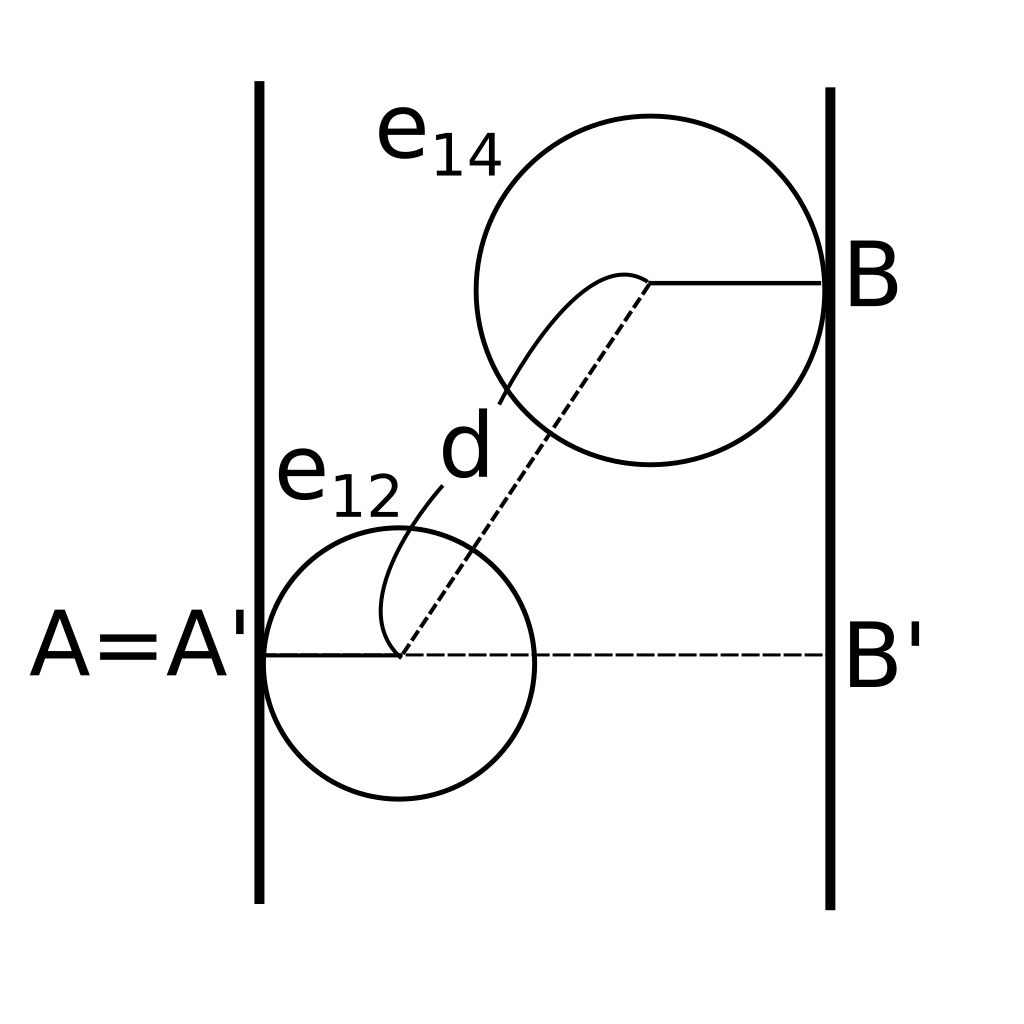
\includegraphics[width=3.5in, height=3.5in,
 keepaspectratio]{./img/HexahedraWithSphericalFaces/sideSliceDistance.png}
 \caption{}
 \label{fig:sideSliceDistance}
\end{figure}

\begin{figure}[h!tbp]
 \centering
 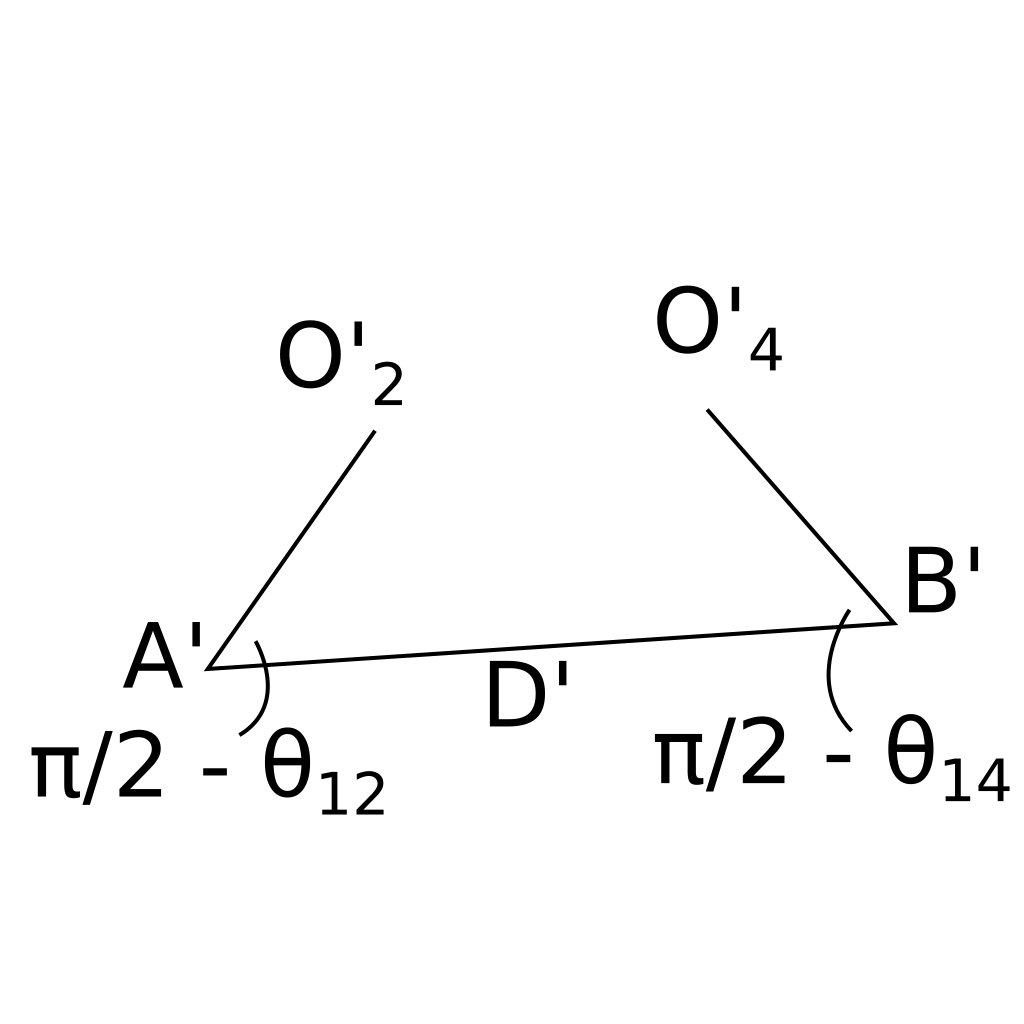
\includegraphics[width=3.5in, height=3.5in,
 keepaspectratio]{./img/HexahedraWithSphericalFaces/adb.png}
 \caption{}
 \label{fig:adb}
\end{figure}
 
\begin{proof}
 (1) Let $\theta'_{24}$ be the face-angle of $O_2$ and $O_4$. From the
 law of cosine, we have
 \begin{eqnarray}
  \overline{O_2O_4}^2 = r_2^2 + r_4^2 - 2r_2r_4\cos(\pi-\theta'_{24})
 \end{eqnarray}
From Figure \ref{fig:adb}, we get a formula
\begin{eqnarray*}
 \overline{O'_2O'_4}^2 = (\overline{A'B'} - r_2\sin\theta_{12}-
  r_4\sin\theta_{14})^2 + (-r_2\cos\theta_{12} + r_4 \cos \theta_{14})^2
\end{eqnarray*}
 Remark that $z_2 = z_A= 0, z_4 = z_B$. Then we have
\begin{eqnarray*}
 \overline{O_2O_4}^2 &=& \overline{O'_2O'_4}^2 + (z_2-z_4)^2\\
 &=&\overline{A'B'}^2 + 2 \overline{A'B'}(-r_2\sin\theta_{12} -
  r_4\sin\theta_{14}) + r^2_2 + r^2_4 -2r_2r_4\cos(\theta_{12} +
  \theta_{14}) + z^2_B
\end{eqnarray*}
Using (2.B) and $\overline{A'B'}^2 + (z_A-z_B)^2 = \overline{AB}^2$,
\begin{eqnarray*}
 \overline{AB}^2 + 2\overline{A'B'}(-r_2\sin\theta_{12} -
  r_4\sin\theta_{14}) - 2r_2r_4\{\cos(\theta_{12} + \theta_{14}) -
  \cos(\pi- \theta'_{24})\} = 0
\end{eqnarray*}
 $r_2, r_4$ satisfy (2.A) and they are positive, so we obtain
\begin{eqnarray*}
 \cos(\theta_{12} + \theta_{14}) = \cos(\pi - \theta'_{24})
\end{eqnarray*}
From Lemma 2.3, $\theta_{12} + \theta_{14} + \theta_{24} = \pi$. It
 follows that $\theta_24 = \theta'_24$. In the same way $\theta_{46}$
 (resp.$\theta{26}$) is equal to the face-angle of $O_4$ and $O_6$(resp
 $O_2$ and $O_6$.)

(2) First we show that two edges $e_{12}$ and $e_{14}$ are mutually tangent
 on $O_1$. The radius of $e_{12}$(resp. $e_{14}$) is
 $r_2\sin\theta_{12}$ (resp. $r_4\sin\theta_{14}$). Let $d$ be the
 distance between two centers of two circles $e_{12}$, $e_{14}$. See
 Figure \ref{fig:sideSliceDistance}.

We have
 \begin{align*}
d^2&= (\overline{A'B'} - r_2\sin\theta_{12}-r_4\sin\theta_{14})^2 + \overline{BB'}^2\\
&= (\overline{A'B'} - \overline{AB}/(2\overline{A'B'}))^2 + \overline{BB'}^2\\
&= \overline{A'B'}^2 - \overline{AB}^2
  +\overline{AB}^4/(4\overline{A'B'}^2) + \overline{BB'}^2\\
&= \overline{AB}^4 / (4 \overline{A'B'}^2)\\
&=(r_2\sin\theta_{12} + r_4\sin\theta_{14})^2\\
d&= r_2\sin\theta_{12} + r_4\sin\theta_{14}
 \end{align*}
It means that $e_{12}$ and $e_{14}$ are mutually tangent.

Next we will show that the edge $e_{24}$ is tangent to both of $e_{12}$ and
 $e_{14}$. Assume that it is not. Then $e_{24}$ intersects to $O_1$
 twice.
(Remark that the tangent point of $e_{12}$ and $e_{14}$ is also on the
 circle $e_{24}$.) But all intersection points of $e_{24}$ and $O_1$ are
 on $e_{12}$ and $e_{14}$ by definition. This contradicts to the fact
 that $e_{12}$ is tangent to $e_{14}$. So the edge $e_{24}$ is tangent
 to both of $e_{12}$ and $e_{14}$. Similarly we will show it about $E$
 and $F$.

\begin{figure}[h!tbp]
  \begin{minipage}[t]{0.3\textwidth}
   \centering
   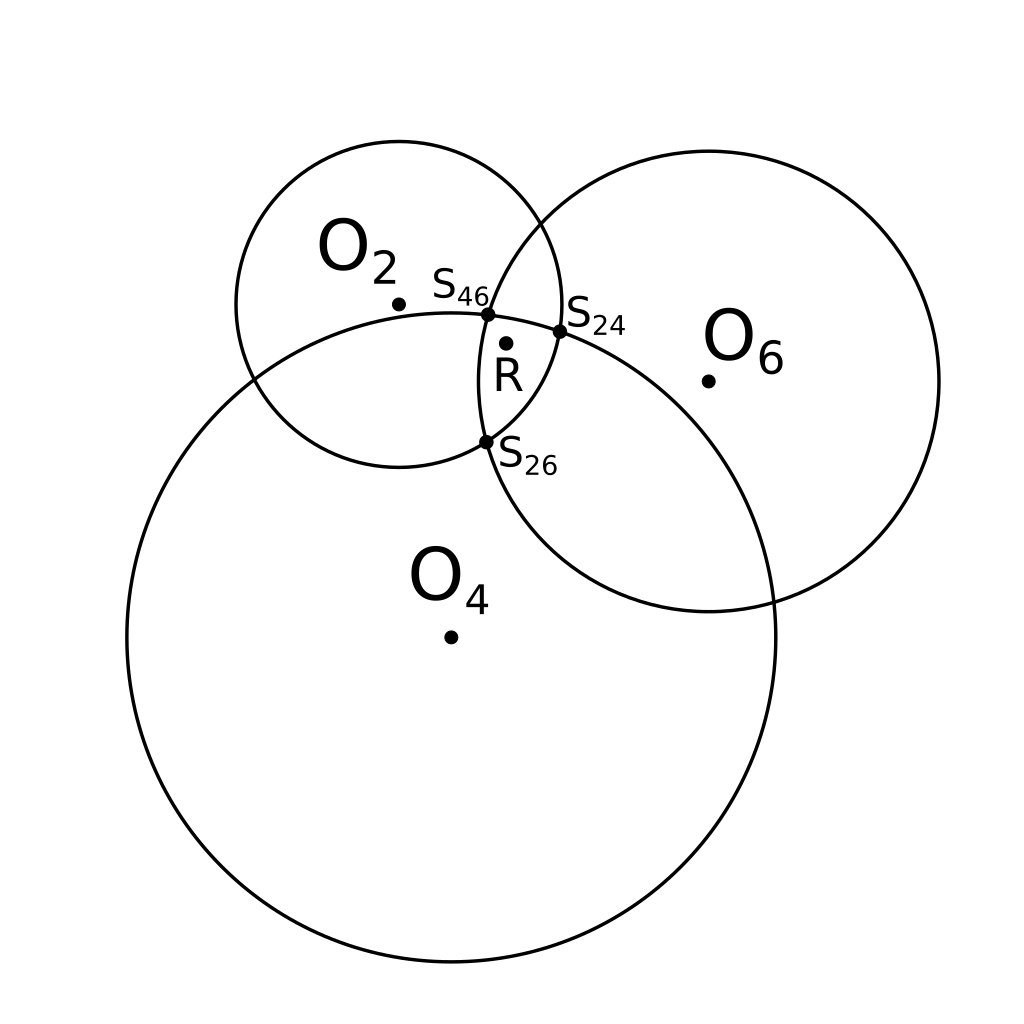
\includegraphics[width=2in, keepaspectratio]{./img/HexahedraWithSphericalFaces/threeCircles1.png}
   \subcaption{}
   \label{fig:}
  \end{minipage}
 \hspace*{\fill}
  \begin{minipage}[t]{0.3\textwidth}
   \centering
   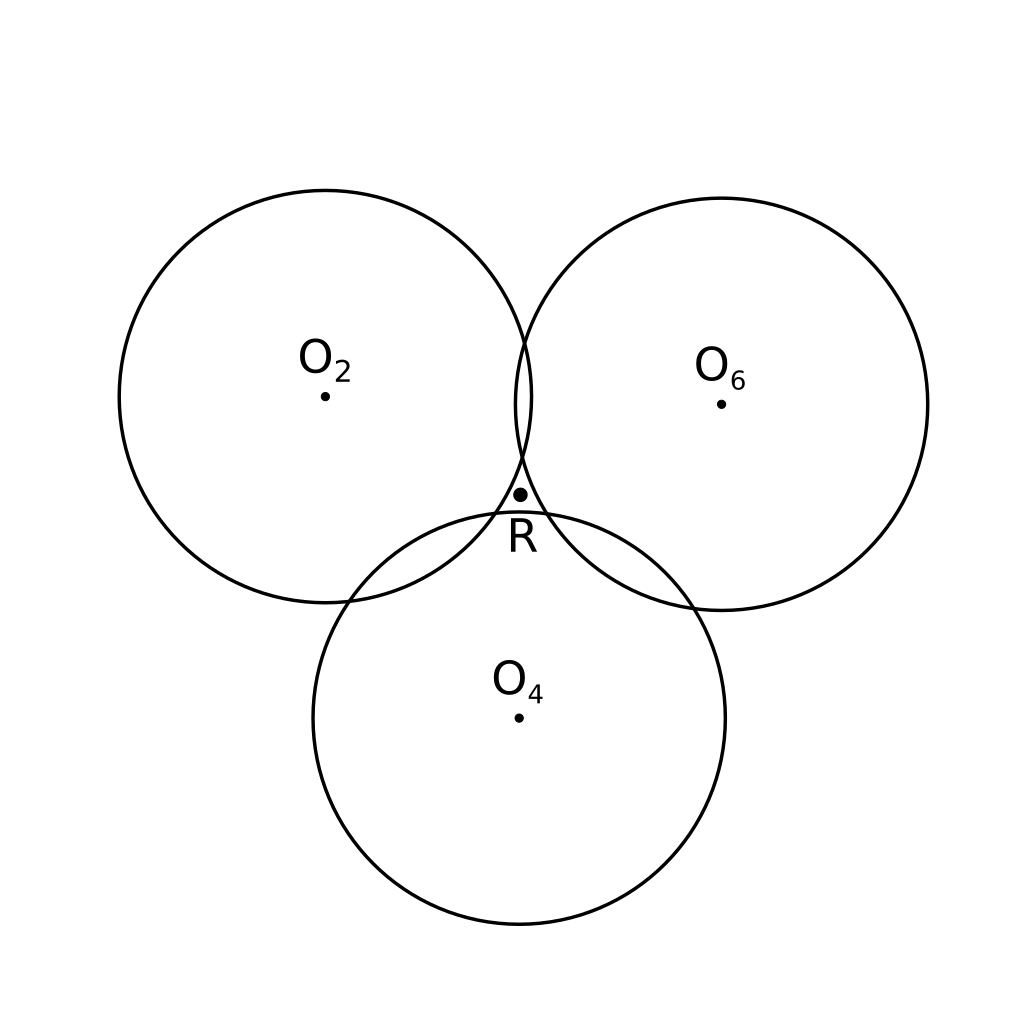
\includegraphics[width=2in, keepaspectratio]{./img/HexahedraWithSphericalFaces/threeCircles2.png}
   \subcaption{}
   \label{fig:}
  \end{minipage}
  \hspace*{\fill}
  \begin{minipage}[t]{0.3\textwidth}
   \centering
   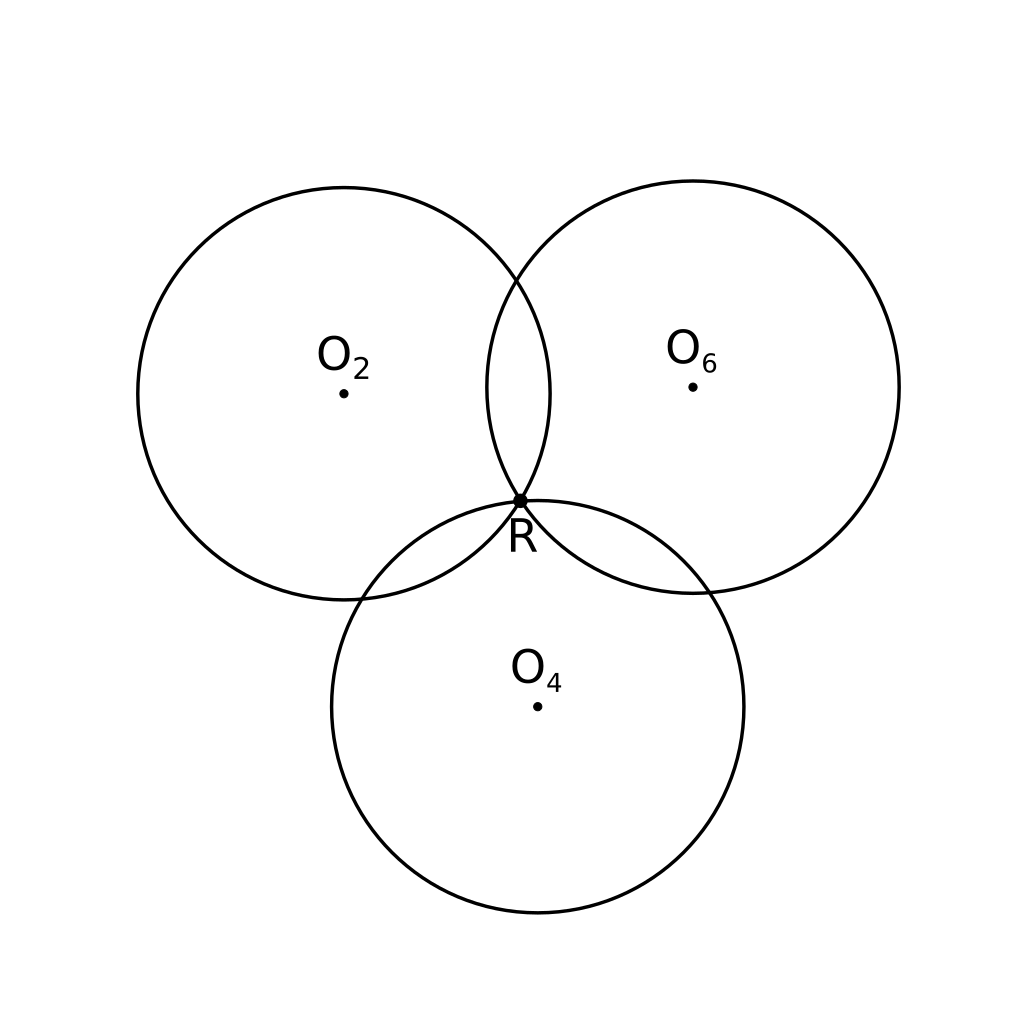
\includegraphics[width=2in, keepaspectratio]{./img/HexahedraWithSphericalFaces/threeCircles3.png}
   \subcaption{\textit{Plastic}}
   \label{fig:3dcolPlastic}
  \end{minipage}
  \caption{\textit{Full-colored printing by DMM.make 3D print.}}
  \label{fig:3dcol}
\end{figure}


(3) Let $\alpha$ be a plane containing 3 centers $O_2, O_4, O_6$. Let
 $C_2, C_4, C_6$ be three circles on $\alpha$ such that $C_i$ is the
 intersection of the sphere $O_i$ and the plane $\alpha$. ($i=2, 4, 6$.)
Let R be the radical point of $C_2, C_4, C_6$. There are three cases
 here.
(i) $R$ is inside if $C_2, C_4, C_6$.(ii) R is outside $C_2, C_4, C_6$.
(iii)$R$ is on $C_2, C_4, C_6$. (See Figure 9)

In the case (i), let three points $S_{24}, S_{46}, S_{26}$ be as in Figure
 9 (left). Here we have $\angle O_2 S_{24} O_4 = \pi - \theta_{24}$,
because their face-angle of $O_2$ and $O_4$ is $\theta_{24}$.
In the same way, $\angle O_4\theta_{46}O_6 = \pi - \theta_{46}$ and
$\angle O_2S_{26}O_6 = \pi-\theta_{26}$ hold. Hence

\begin{align*}
 \angle O_2 S_{24} O_4 + \angle O_4 S_{46} O_6 + \angle O_2 S_{26} O_6 = 3\pi -
 \theta_{24} - \theta_{46} - \theta_{26} = 2\pi.
\end{align*}

On the other hand, from Figure 9 (left)

\begin{align*}
 \angle O_2 S_{24} O_4 &< \angle O_2 R O_4
 \angle O_2 S_{24} O_4 &< \angle O_2 R O_4
 \angle O_2 S_{24} O_4 &< \angle O_2 R O_4
\end{align*}
and
\begin{align*}
 \angle O_2 R O_4 + \angle O_4 R O_6 + \angle O_2 R O_6 = 2\pi
\end{align*}
This is a contradiction. So this case cannnot happen. In the same way,
 the case (ii) cannnot happen. These follow that the radical point $R$
 is on the intersection of 3 circles $C_2, C_4, C_6.$ this means that
 $R$ is the unique intersection of 3 spheres $O_2, O_4, O_6$. this must
 be $G$.

(4) The 6-pre ($O_1, ..., O_6$) satisfies (P1) by definition.

(P2): For $(i, j) = (1, 3), (3, 5), (1, 5)$, it is good because we first
 take a triangle prism (consisting of $O_1, O_3, O_5$) with face-angles
 $\theta_{13}, \theta_{35}, \theta_{15}.$ 
For $(i, j) = (1, 2), (1, 4), (4, 5), (5, 6), (2, 3), (3, 6)$, it is
 good from Lemma\ref{angles}. In other cases, it is good from Theorem
 \ref{compat}(1).

(P3): At $H = \infty, AH, BH, CH$ are parallel lines so they are tangent
 at $\infty$. At $D, R, F, G,$ we have shown it in Theorem \ref{compat}(2)(3).
\end{proof}

\subsection{Parameter space}
In this subsection we first consider in the case that $n_{ij} = 3$ for all
$(i, j) \in E$. (That is, in case (a) in Lemma \ref{combination}) There are 11 cases
in Lemma \ref{combination} The case (a) is not a special case, and we can make
similar observation in other cases.
The linear equations (2.A) are:
\begin{align*}
 r_2 + r_4 &= (3 + z_B^2) / 3 \\
 r_4 + r_6 &= (3 + (z_B - z_C)^2 ) / 3 \\
 r_2 + r_6 &= (3 + z_C^2) / 3
\end{align*}

Here $\overline{A'B'} = \overline{B'C'} = \overline{A'C'} = \sqrt{3}$
because $\Delta{A'B'C'}$ is a regular triangle and the radius of the
circumcircle is 1.(In all cases, $\overline{A'B'} = 2\sin\theta_{35},
\overline{B'C'} = 2\sin\theta{13}, \overline{A'C'} = 2\sin\theta{15}$.)
We solve these equations and we have 
\begin{align}
 r2 &= (-2z_Bz_C + 2Z^2_C + 3) / 6 \\
 r4 &= (2z_Bz_C + 3) / 6 \\
 r6 &= (2z^2_B - 2z_Bz_c + 3) / 6.
\end{align}
First we assume that $r_2, r_4, r_6$ are positive. This condition is
equivalent to the followings.
\begin{align}
 -3 / 2 &< -z_Bz_C + z^2_C\\
 -3 / 2 &< z_Bz_C \\
 -3 / 2 &< z^2_B - z_Bz_C
\end{align}
So we assume (3.B). We will determine $O_1, ... , O_6$ as in the
previous section. It is clear that 6 faces $O_1, ... , O_6$ surround
a hexahedron if and only if $O_2$ doesn't interest to $O_5$ nor $O_3$
doesn't intersect to $O_4$ nor $O_1$ doesn't intersect to $O_6$.

$O_2$ doesn't interest to $O_5$ if and only if the distance from the center
of the sphere $O_2$ to the plane $O_5$ is more than $r_2$. In this case
the distance is $3 / 2 - r_2$ and hence $O_2$ doesn't intersect to $O_5$
if and only if $r_2 < 3/4$. In the same way $r_4 < 3/4$ and $r_6 <
3/4$. These three inequalities are equivalent to
\begin{align}
 -z_Bz_C + z^2_C &< 3 / 4\\
 z_Bz_C &< 3 / 4 \\
 z^2_B - z_B z_C &< 3/ 4
\end{align}

See Figure 10 ($z_B, z_C$) in the shaded area of this figure satisfies
all of(2.D) an (2.E) and $z_B \geq 0$.

In case (a), original three parameters $z_A, z_B, z_C$ have symmetry,
because $O_1, O_3, O_5$ form a \textit{regular} triangle prism.
If $z_C < 0$ then we exchange the roles of $z_A$ and $z_C$ and we can reduce
($z_B, z_C$) to ($z_B - z_C, -z_C$) in the case of $z_C > 0$.
If $z_B \leq z_C < 2z_B$ then we exchange the roles of $z_B$ and $z_C$
and we can reduce $(z_B, z_C)$ to $(z_C -z_B,z_C)$ in case of 
$z_C \geq 2z_B$. In this way, the correct parameter space is as in Figure
11.

Here two hyperbola $z^2_C - z_bz_C = 3/4$ and $z_B z_C = 3/4$ intersects
at ($\sqrt{6} / 4, \sqrt{6}/2$) and this point is on the straight line
$z_C=2z_B$. In Figure 11, points on $z^2_C - z_Bz_C = 3/4$ aren't
contained in the area. When ($z_b, z_C$) is on this parabola, the face
$O_2$ is tangent to $O_5$. Moreover when
$(z_B, z_C) = (\sqrt{6} / 4, \sqrt{6}/2)$, the face $O_3$ is also tangent
to $O_4$.
In the same way, we have a similar result in case $(b), (c), (d), (e),
(h), (i)$. The figures below are parameter space in each case.

In case $(f), (g), (j) and (k)$, there are no solution of $(z_B, z_C)$
to be a hexahedron. In fact, in case (f),
\begin{align*}
\begin{cases}
 0 &< \dfrac{z_Bz_C}{\sqrt{3}} < \dfrac{\sqrt{3}}{4} \\
 0 &< \dfrac{1 + z^2_B - z_Bz_C}{2} < \dfrac{1}{2} \\
 0 &< \dfrac{3 + z^2_C - z_Bz_C}{2\sqrt{3}} < \dfrac{\sqrt{3}}{2}.
\end{cases}
\end{align*}
In case (g),

\begin{align*}
\begin{cases}
0 &< \dfrac{z_Bz_C}{2} < \dfrac{\sqrt{3}}{2 + \sqrt{3}} \\
0 &< \dfrac{2 + 2z^2_B - z_Bz_C}{4} < \dfrac{1}{2} \\
0 &< \dfrac{\sqrt{3}(6 + 2z^2_C - 3z_Bz_C)}{12} < \dfrac{\sqrt{3}}{2}
\end{cases}
\end{align*}

In case (j),

\begin{align*}
 \begin{cases}
  0 &< \dfrac{z_Bz_C}{2} < \dfrac{1}{2}\\
  0 &< \dfrac{\sqrt{2}(2 + z^2_B - z_B z_C)}{4} < \dfrac{\sqrt{2}}{2}\\
  0 &< \dfrac{\sqrt{2}(2 + z^2_C - z_B z_C)}{4} < \dfrac{\sqrt{2}}{2}
 \end{cases}
\end{align*}

In case (k),

\begin{align*}
 \begin{cases}
  0 &< \dfrac{2z_Bz_C}{\sqrt{6} + \sqrt{2}} < \dfrac{1}{\cos(\pi/12+1)}\\
  0 &< \dfrac{\sqrt{2}(2 (1 + \sqrt{3}) + (1 + \sqrt{3})z^2_B -2z_Bz_C)}
  {2(\sqrt{6} + \sqrt{2})} < \dfrac{\sqrt{2}}{2}\\
  0 &< \dfrac{\sqrt{2}(2 (1 + \sqrt{3}) + (1 + \sqrt{3})z^2_C
  -2\sqrt{3}z_Bz_C)}
  {2(\sqrt{6} + \sqrt{2})} < \dfrac{\sqrt{2}}{2}
 \end{cases}
\end{align*}
In these cases, there is no answer for ($z_b, z_C$).

We complete the proof of the main Theorem \ref{main}.

\subsection{Group $G$ and the limit set $\Delta(G)$}
Let $\gamma_i \in \text{M\"ob}(S^3)$ be the inversion of $O_i$ for $i =
1,...,6$.
Let $G'$ be a group generated by $\gamma_i$'s. From Condition (P2), we
have relations
\begin{align*}
 (\gamma_i \gamma_j)^{n_{ij}} = 1
\end{align*}
for $(i, j) \in E.$ (Here $1$ is the identity map.) If $(i, j) \notin E$,
there are no relation between $\gamma_i$ and $\gamma_j$.
And at each vertex, three edges with the vertex are mutually tangent,
there are no more relations. So we have that
\begin{align*}
 \tilde G = <\gamma_1, ...,\gamma_6 | (\gamma_i\gamma_j)^{n_{ij}} = 1 for
 (i, j) \in E.>
\end{align*}
The length of all relations are even, so we can consider a set $G = G(P)$
of elements of even length. $G$ is a subset of $G'$. Here we remark
that each $\gamma_i$ is a inversion and it is orientation reversing. So
each element of $G$ is orientation preserving M\"obius transformation.
It follows that $G$ is a subset of M\"ob$_+(S^3)$.

In the previous subsection we got a parameter space for $P$ to be a
hexahedron with the initial conditions. Here are some pictures of the
limit sets $\Gamma(G)$. However, if we take $O_1, ..., O_6$ as in the
previous section, the limit set contains a infinity point $\infty$. So
we transform $\O_1, ..., O_6$ by an inversion of a proper sphere in
order to make $\Gamma(G)$ doesn't contain the infinity point.

Only when $(z_B, z_C) =(0, 0), \Delta(G)$ is a round sphere and hence
$G$ is fuchsian. In other cases we get a homotopy to the case 
$(z_B, z_C) = (0, 0)$, we know that $G$ is quasi-fuchsian.

\subsection{Extended Schottky group for a cube with spherical faces}\label{extend}
If $(O_1, ..., O_6)$ gives a polyhedron with conditions
$(P1), (P2), (P3)$.
These spheres also define a Schottky type subgroup of M\"ob$_+(S^3)$ 
only in case (a). Indeed we have the following  proposition.

\begin{proposition}
Let $\{n_{ij}\}$ be of type (a) in Lemma \ref{combination}. Then there exist three
 (orientation preserving) transformations $f_1, f_2, f_3$ such that
 \begin{description}
  \item[(1)] $f_1$ maps the inside of $O_1$ onto the outside of
             $O_6$, $f_1(H) = C$, $f_1(A) = F$,  $f_1(D) = G$, and
             $f_1(B) = E$.
  \item[(2)] $f_2$ maps the inside of $O_3$ onto the outside of
             $O_4$, $f_2(H) = B$, $f_2(A) = D$,  $f_2(F) = G$, and
             $f_2(C) = E$.             
  \item[(3)] $f_3$ maps the inside of $O_5$ onto the outside of
             $O_2$, $f_3(H) = A$, $f_3(B) = D$,  $f_3(E) = G$, and
             $f_3(C) = F$.
\end{description}
\end{proposition}

Let $H$ be a sub group of M\"ob$_+(S^3)$ generated by $f_1, f_2,
f_3$. This proposition follows that
\begin{align*}
 H = <f_1, f_2, f_3|(f_1f_2)^3 = (f_2f_3)^3 = (f_1f_3)^3 = e>.
\end{align*}
It is easy to show that the fundamental domain of $H$ is a polyhedron
surrounded by the initial spheres. The limit set $H$ is the same as that
of $G$.

\begin{proof}
See Figure \ref{fig:infTriangle}. Since we assume that $n_{ij} = \pi/3$, we have
\begin{align*}
 A(1, 0, 0), B(-\frac{1}{2}, z_B), C(-\frac{1}{2}, -\frac{\sqrt{3}}{2}, z_C).
\end{align*}
\end{proof}

Let $O_2$ be the center of the spheres $O_2$, then we have
\begin{align*}
 O_2(1 - r_2, 0, 0).
\end{align*}
From Lemmma\ref{eightVertices}, 7 points A, B, C, D, E, F, G lie on one plane. D is on
the segment $AB$ and
\begin{align*}
 AD : DB = r_2\sin\theta_{12} : r_4\sin\theta_{14} = r_2 : r_4
\end{align*}
See Figure \ref{fig:sideSlice}. In the same way we have
\begin{align*}
 BE : EC &= r_4\sin\theta_{45} : r_6\sin\theta_{56} &= r_4:r_6\\
 CF : FA &= r_6\sin\theta_{36} : r_2\sin\theta_{23} &= r_6:r_2
\end{align*}
Using these, we have coordinates of $E$. In fact,
\begin{align*}
 E(-\dfrac{1}{2},\dfrac{\sqrt{3}}{2}\dfrac{r_6-r_4}{r_6 + r_4},
 \dfrac{z_Br_6 + z_C r_4}{r_6 + r_4}).
\end{align*}
And we have
\begin{align*}
 \dfrac{AD}{DB} \cdot \dfrac{BE}{EC} \cdot \dfrac{CF}{FA} = \dfrac{r_2r_4r_6}{r_4r_6r_2} = 1
\end{align*}
From Ceva's theorem, the three lines $AE$, $BF$, and $CD$ meet at one
point. Let $G'$ be the intersection. Using Menelaus's theorem, we have
$AG':G'E = r_2r_4 + r_2r_6:r_4r_6$ and
\begin{align*}
 G' = \dfrac{1}{R}(r_4r_6 - \dfrac{1}{2}(r_2r_4 + r_2r_6), 
 \dfrac{\sqrt{3}}{2}r_2(r_6 - r_4), r_2(z_Br_6 + z_Cr_4)),
\end{align*}
where $R = r_2r_4 + r_4r_6 + r_6r_2.$ It follows that
\begin{align*}
 \overline{O_2G'}^2 = (1 - r_2 - \dfrac{1}{2R}(2r_4r_6 - (r_2r_4 +
 r_2r_6)))^2 + \dfrac{3r^2_2}{4R^2}(r_6 - r_4)^2 +
 \dfrac{r_2^2}{R^2}(z_Br_6 + z_Cr_4)^2
\end{align*}
Using Proposition \ref{angles} we have $\overline{O_2G'} = r_2$. Remark that we
use equations $z_B^2 = 3(r_2 + r_4 - 1), z_C^2 = 3(r_2 + r_6 - 1)$, and
$2z_Bz_C = 6r_2 - 3$.

In the same way we get $\overline{O_4G'} = r_4$ and 
$\overline{O_6G'} = r_6$. These mean that $G' = G$.

From Lemma \ref{sameCircle} $B, D, G, E$ are on one circle. Hence
$CE \cdot CB = CG \cdot CD$. In the same way we obtain 
$CG \cdot CD = CF \cdot CA$. So let $O$ be a sphere with center $C$ and
radius $\sqrt{CE \cdot CB}$ and let $f_O$ be the inversion of $O$
The above two equations follows that
\begin{align*}
 f_O: A \mapsto F, D \mapsto G, B \mapsto E, H \mapsto C.
\end{align*}
Let $f_{O_1}$ be the inversion of $O_1$. $f_{O_1}$ fixes $H, A, D, B$.
Let $f_1 := f_O \circ f_{O_1}$.
$f_1$ is an orientation preserving M\"obius transformation and
\begin{align*}
 f_1 : A \mapsto F, D \mapsto G, B \mapsto E, H \mapsto C.
\end{align*}
It is easy to check that $f_1(O_1) = O_6$ because a sphere is determined
by four points on it. And also $f_1$ maps the inside of $O_1$ to the
outside of $O_6$. Here the inside of $O_1$ means the area which doesn't
contain the prism consistint of $O_1, O_3, O_5$. The we finish the
proof.

Remark:
In other cases $(b),...,(j)$, we don't have a similar result. Three
segments $AE, BF, CD$ meets at one point only in case $(a), (f), (j)$, but
there isn't a parameter space in cases $(f)$ nor $(j)$.


\section{Various Sphairahedra}

In this section, we show other type of the sphairahedra based on up to hexahedron.
We can consider the same problem for other polyhedra. Here is a list of
pentahedra and hexahedra with the number of combination of face-angles
and the dimension of $\tilde{\varepsilon}(n_{ij})$.
classification problems besed on cube type hexahedron.

Ahara, Araki, and Kageyama dealed with only cube.
Nakamura draw sphairahedra based on up to hexahedra and compute
parameter space of them.
In this section, we describe them.

\subsection{Tetrahedron}

\begin{figure}[h!tbp]
  \begin{minipage}[t]{0.23\textwidth}
   \centering
   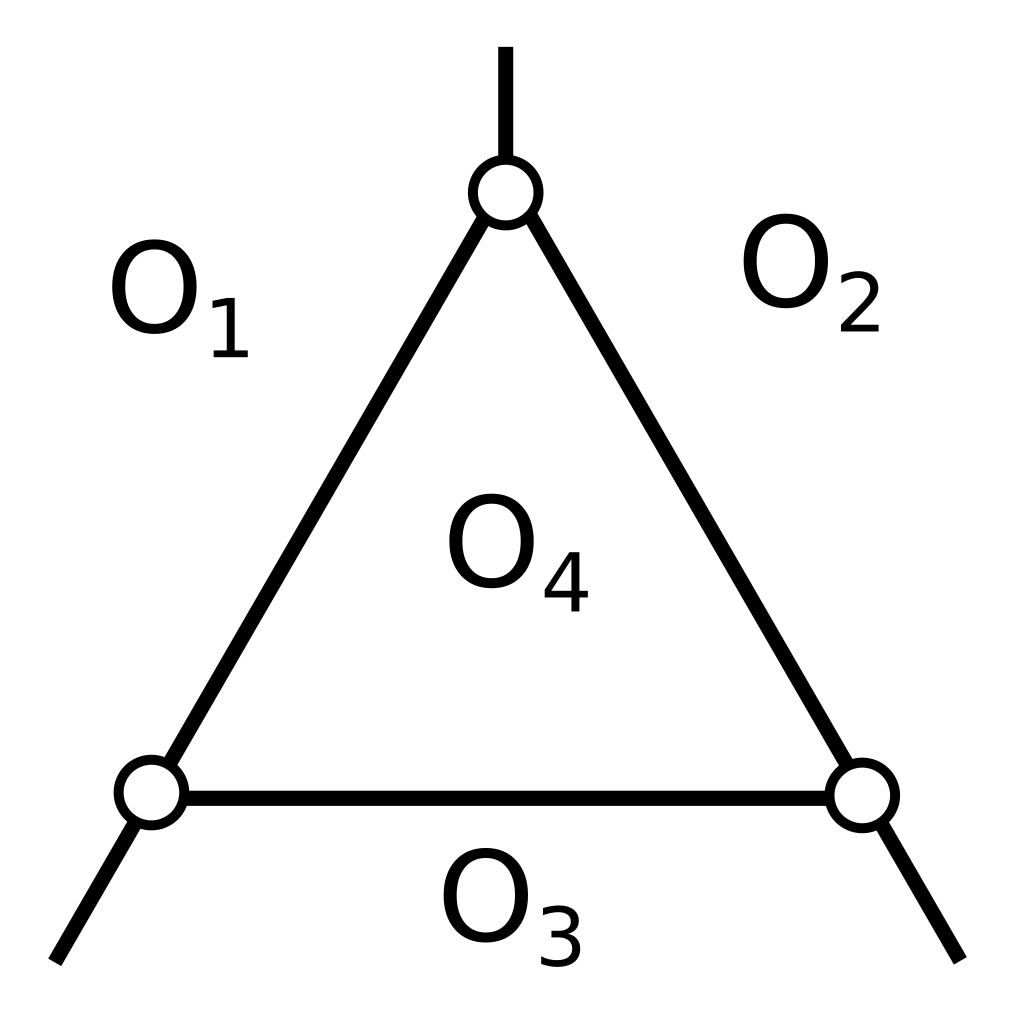
\includegraphics[width=1in, keepaspectratio]{./img/HexahedraWithSphericalFaces/tetrahedron/tetrahedronFaces.png}
   \subcaption{}
   \label{fig:}
  \end{minipage}
 \hspace*{\fill}
  \begin{minipage}[t]{0.23\textwidth}
   \centering
   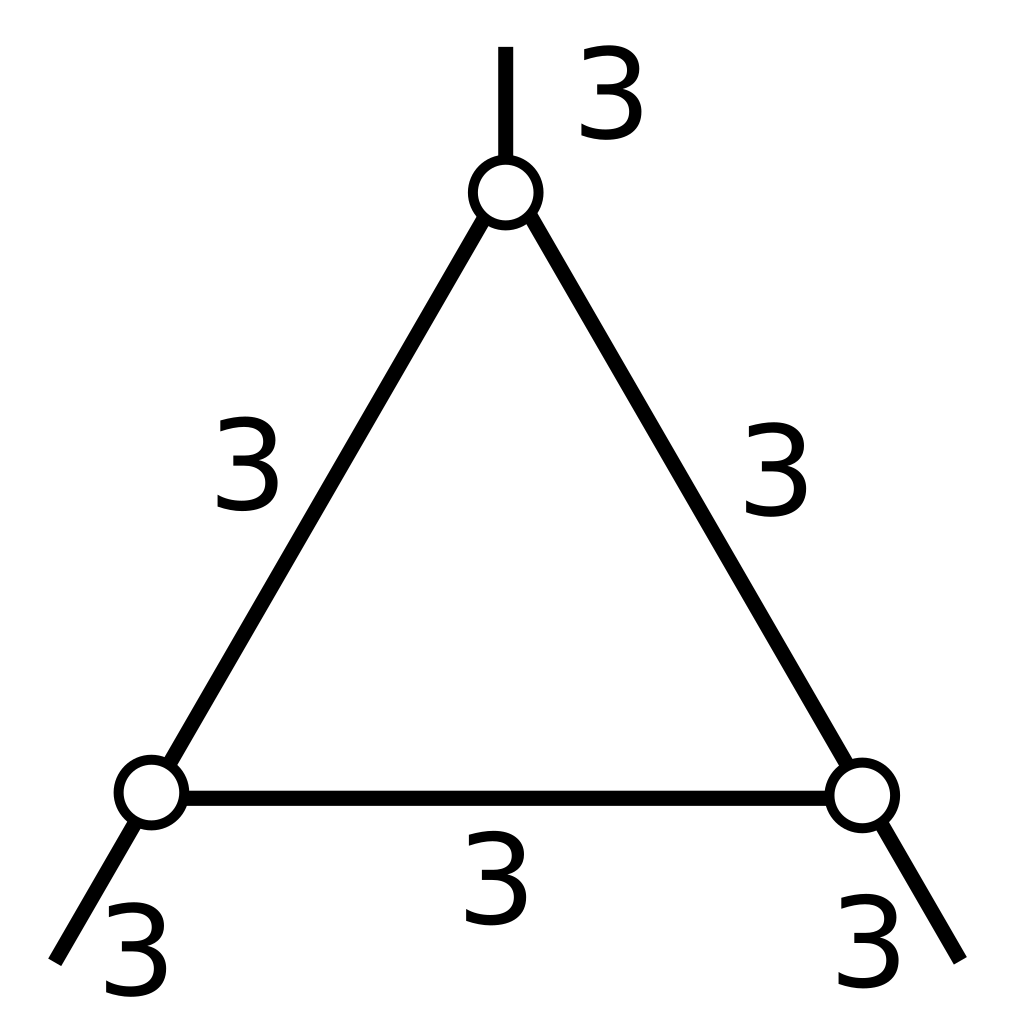
\includegraphics[width=1in,
   keepaspectratio]{./img/HexahedraWithSphericalFaces/tetrahedron/tetrahedron_a.png}
   \subcaption{}
   \label{fig:}
  \end{minipage}
  \hspace*{\fill}
  \begin{minipage}[t]{0.23\textwidth}
   \centering
   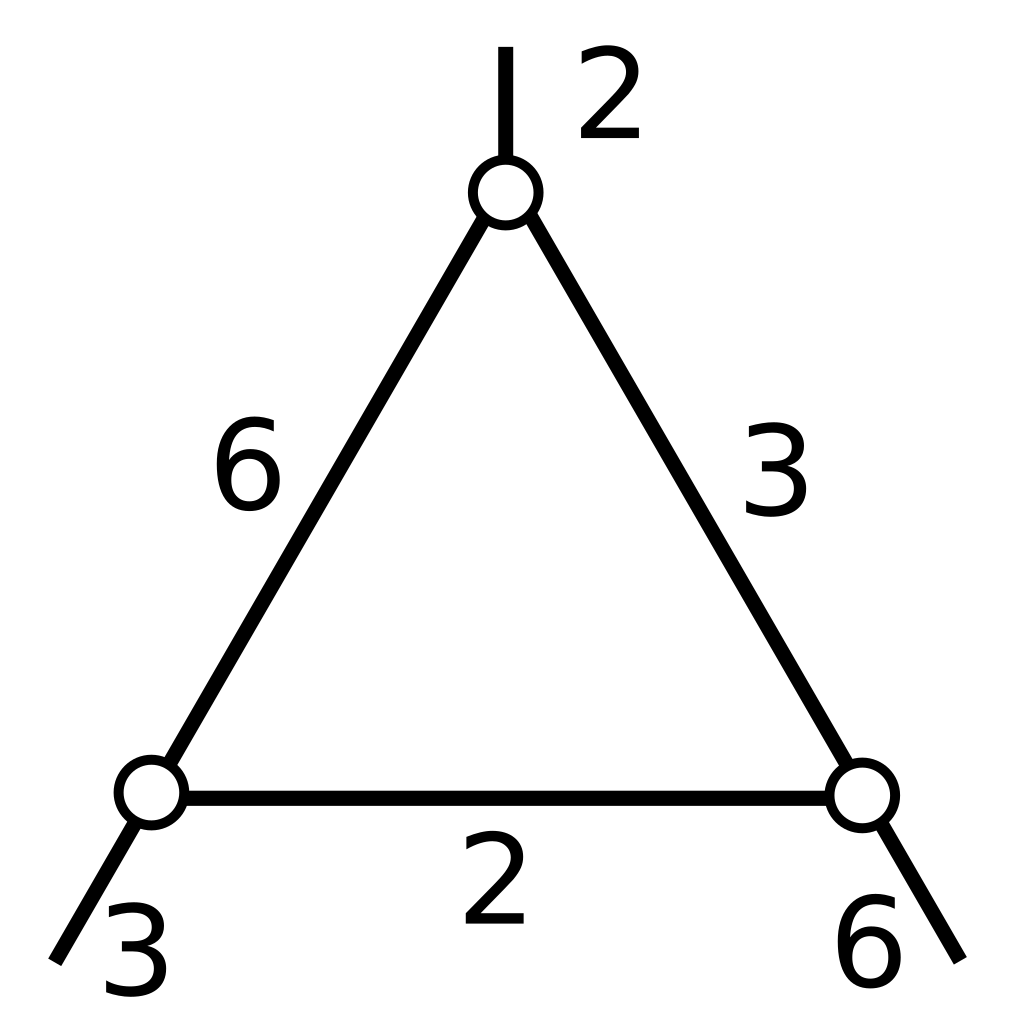
\includegraphics[width=1in, keepaspectratio]{./img/HexahedraWithSphericalFaces/tetrahedron/tetrahedron_b.png}
   \subcaption{}
   \label{}
  \end{minipage}
 \hspace*{\fill}
  \begin{minipage}[t]{0.23\textwidth}
   \centering
   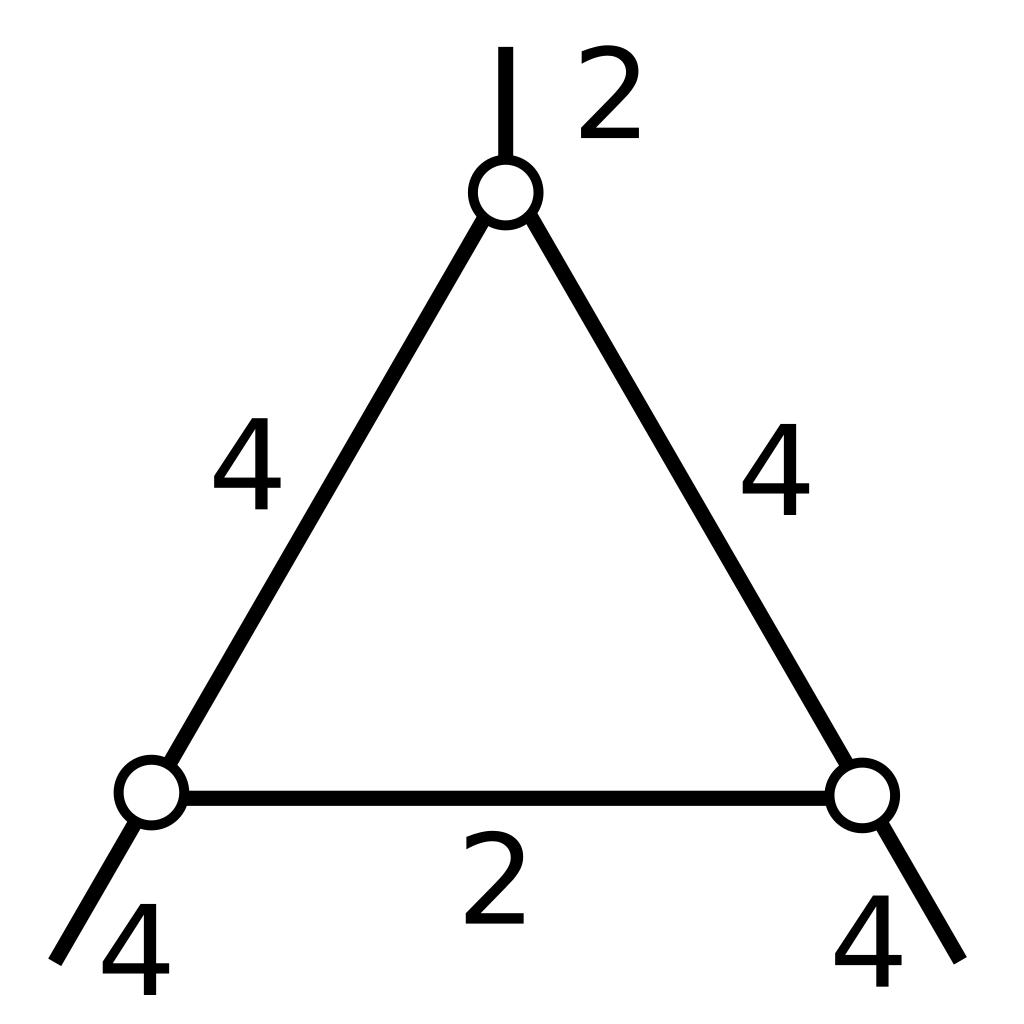
\includegraphics[width=1in, keepaspectratio]{./img/HexahedraWithSphericalFaces/tetrahedron/tetrahedron_c.png}
   \subcaption{}
   \label{fig:}
  \end{minipage}
 \hspace*{\fill}
  \caption{\textit{Full-colored printing by DMM.make 3D print.}}
  \label{fig:}
\end{figure}

\begin{figure}[H]
 \begin{minipage}{0.5\textwidth}
  \begin{minipage}[t]{0.24\textwidth}
   \centering
   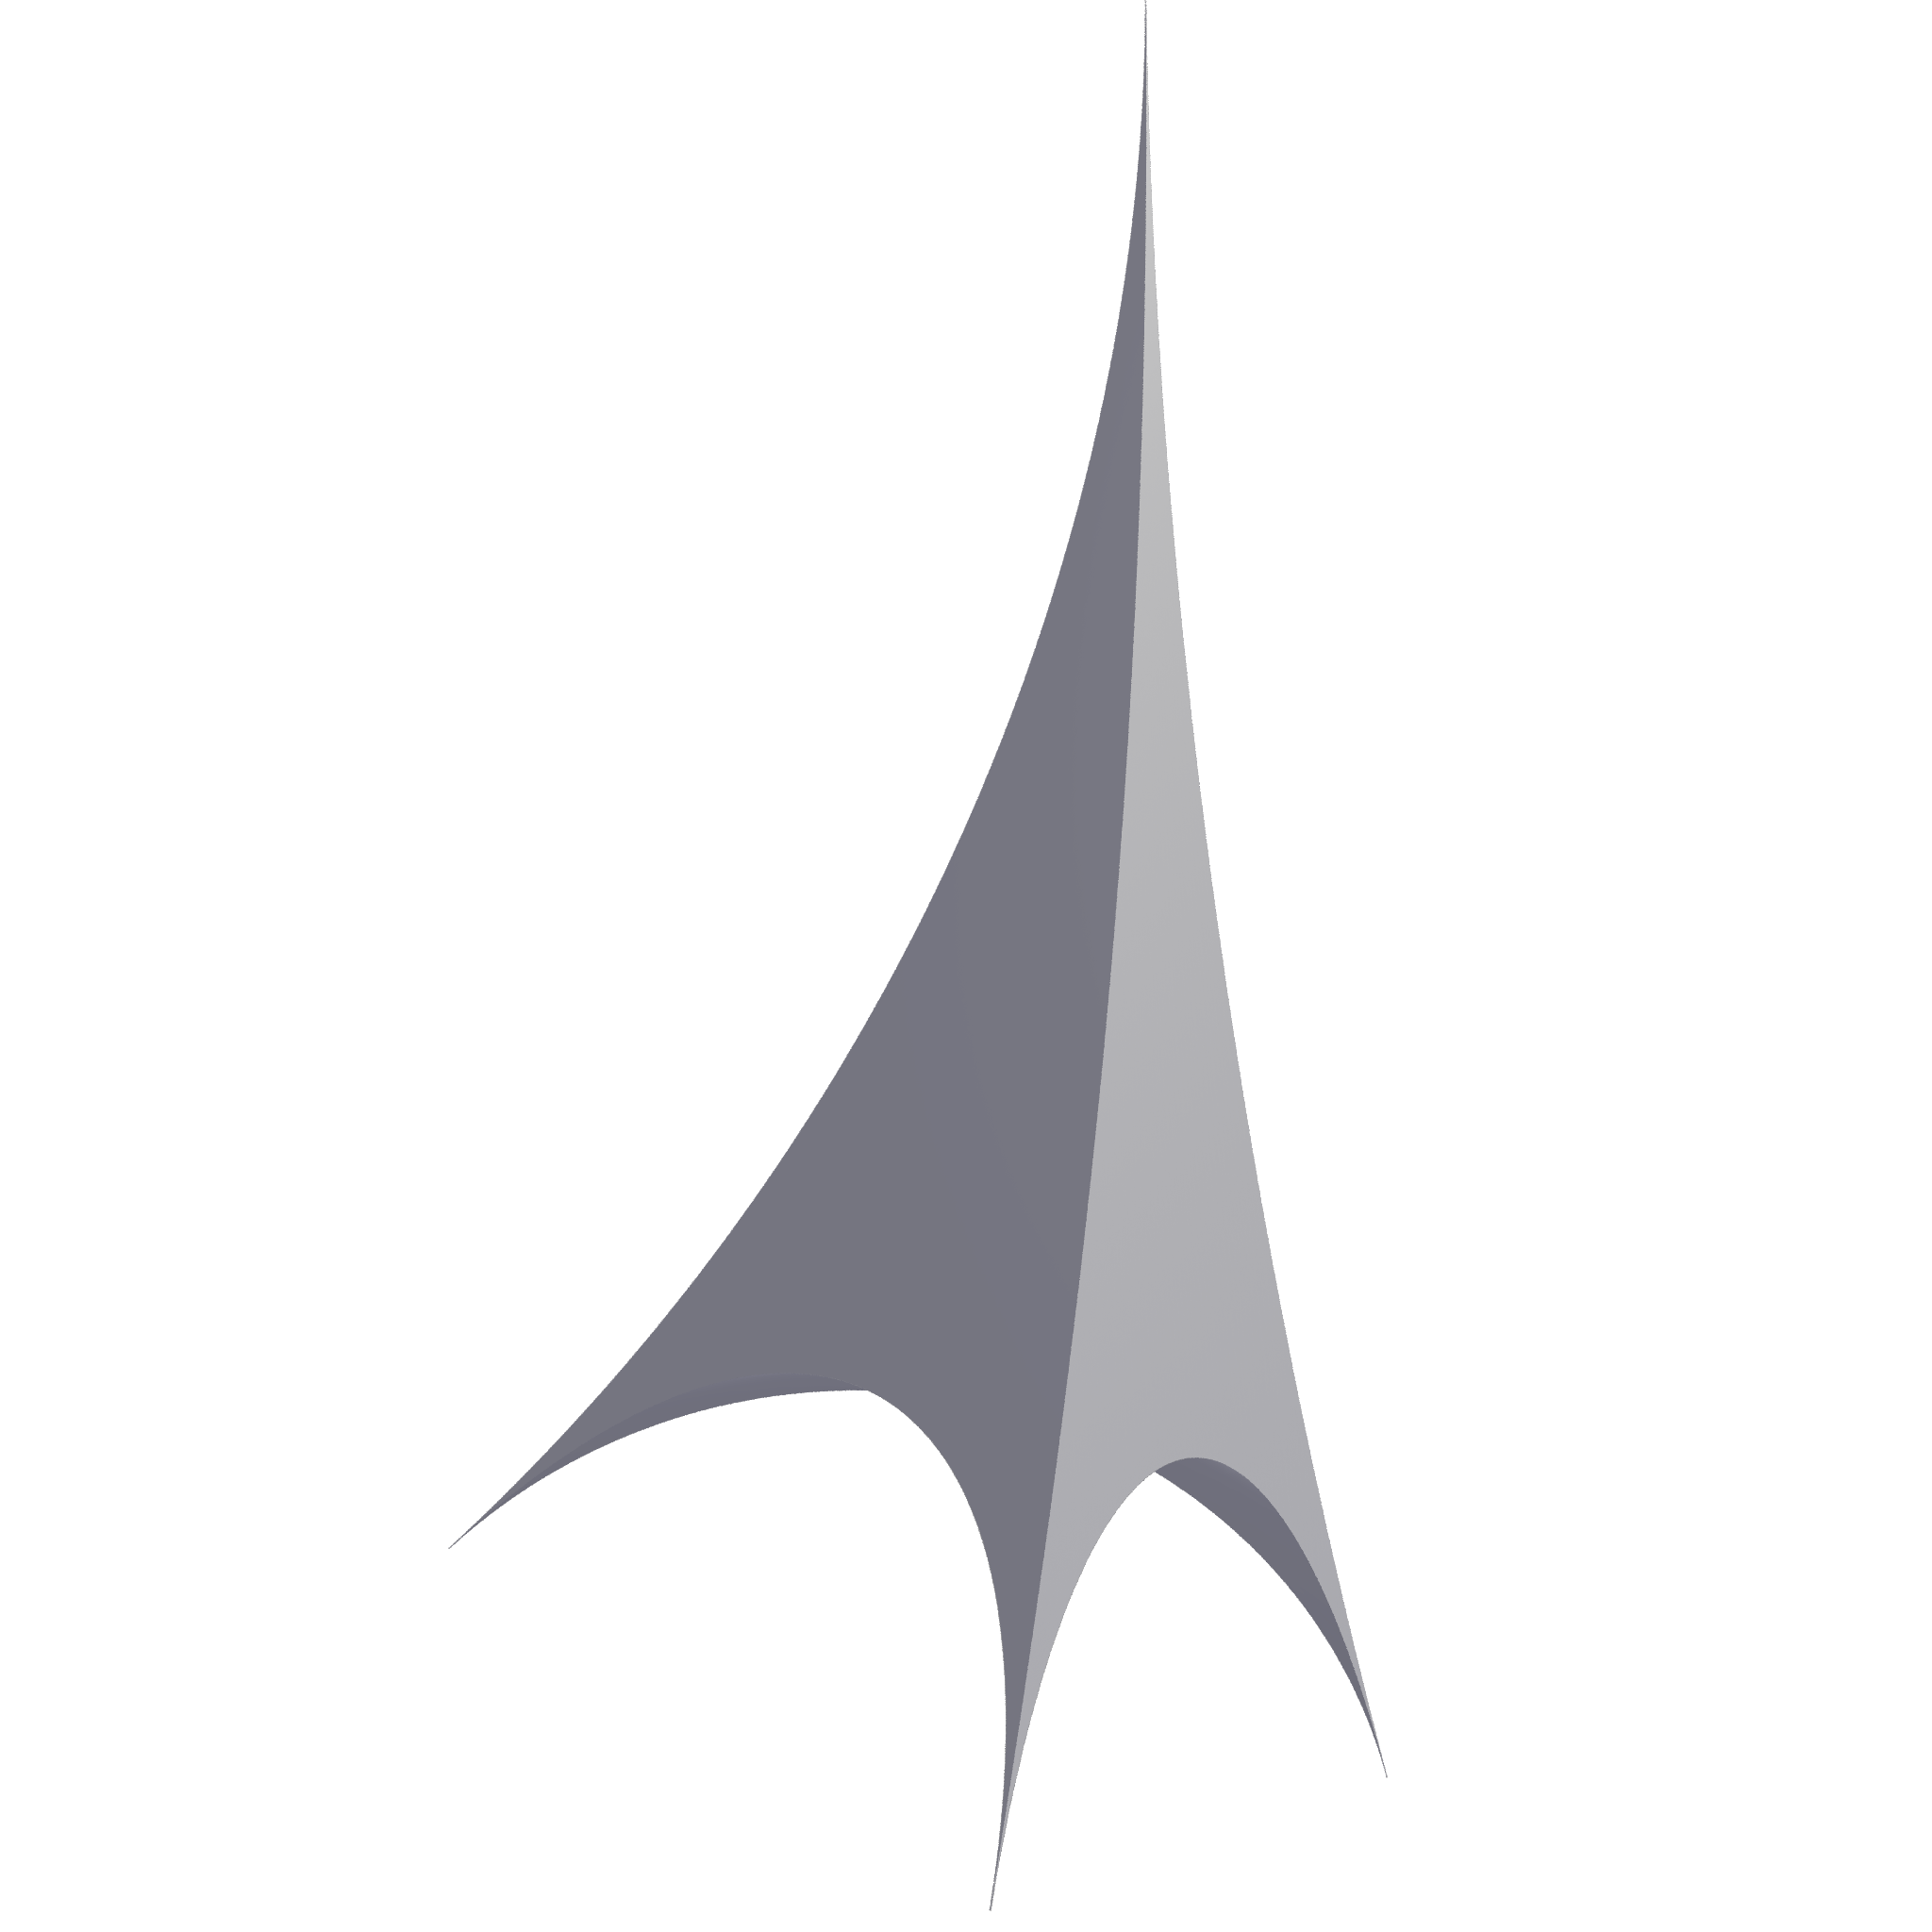
\includegraphics[width=1.35in, height=1.35in, keepaspectratio]{./img/sphairahedron/tetrahedron/sphairahedronFinite.png}
   \subcaption{\textit{Sphairahedron}}
  \end{minipage}
  \hspace*{\fill}
  \begin{minipage}[t]{0.24\textwidth}
   \centering
   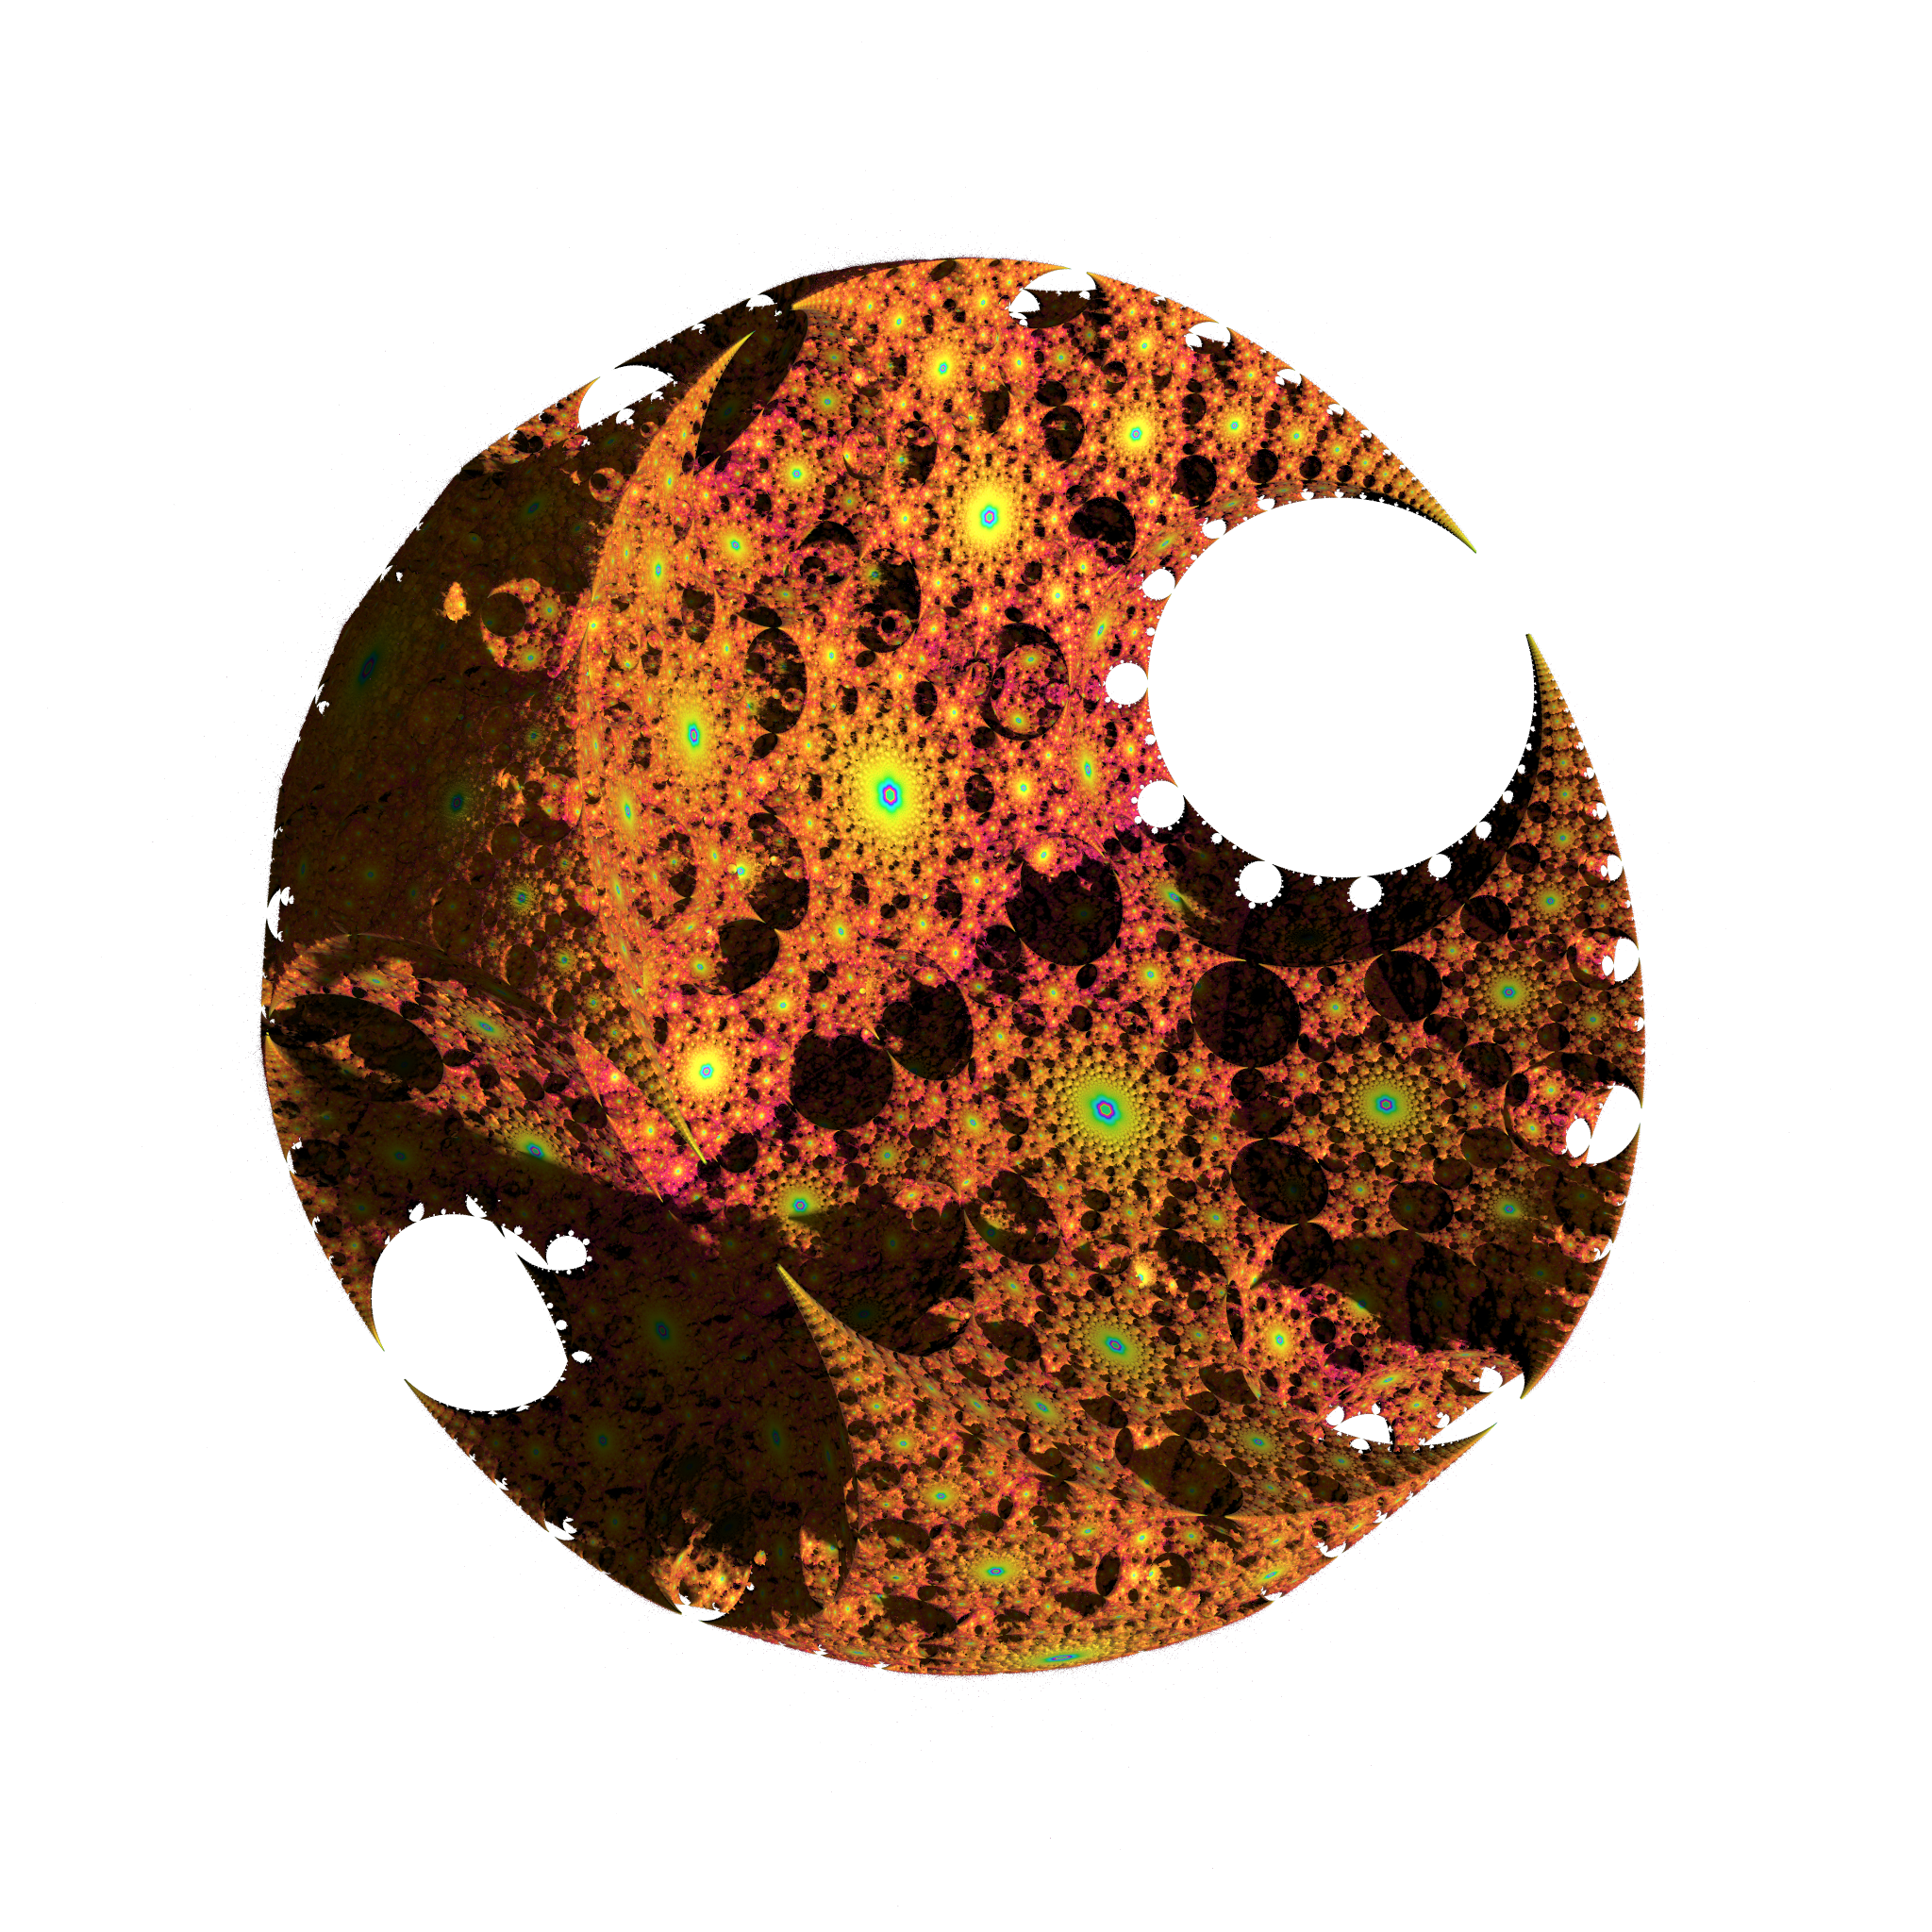
\includegraphics[width=1.35in, height=1.35in, keepaspectratio]{./img/sphairahedron/tetrahedron/limitsetFinite.png}
   \subcaption{\textit{Limit set}}
  \end{minipage}
  \hspace*{\fill}
  \caption{\textit{Finite tetrahedron type.}}
  \label{fig:tetrahedronFinite}
 \end{minipage}
 \hspace*{\fill}
 \begin{minipage}{0.5\textwidth}
  \begin{minipage}[t]{0.24\textwidth}
   \centering
   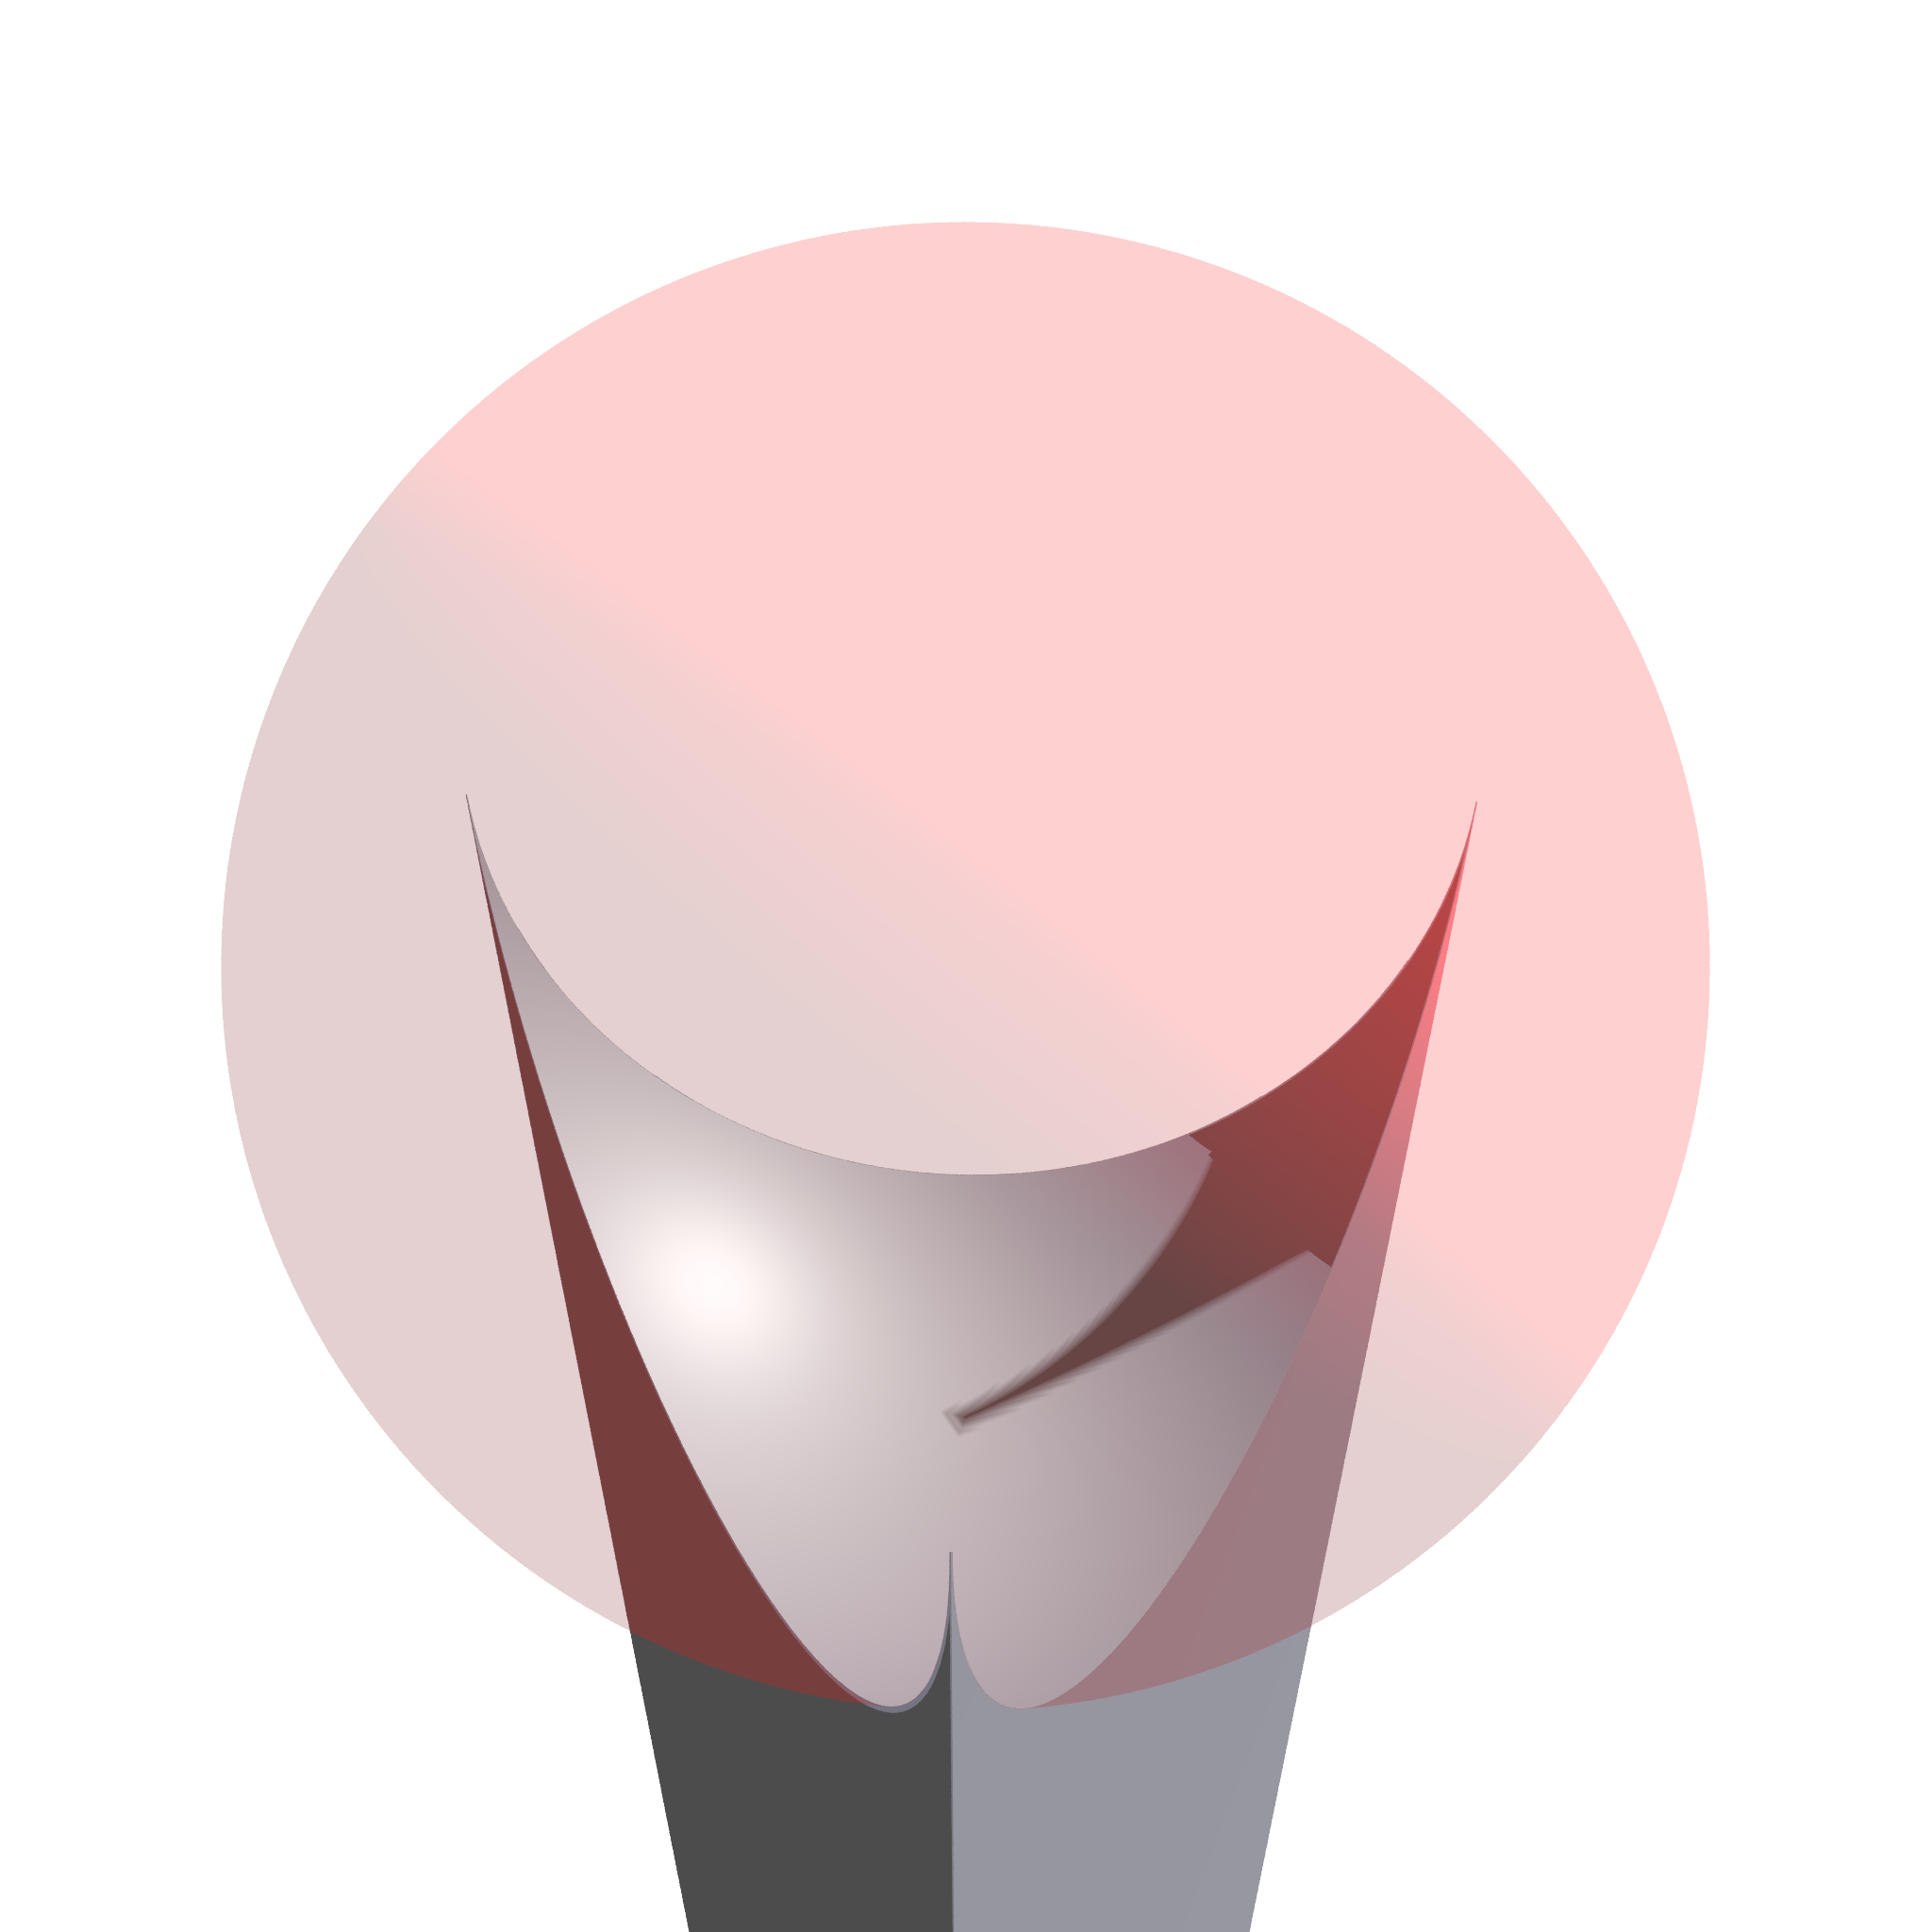
\includegraphics[width=1.35in, height=1.35in, keepaspectratio]{./img/sphairahedron/tetrahedron/sphairahedronInf.png}
   \subcaption{\textit{Sphairahedron}}
  \end{minipage}
  \hspace*{\fill}
  \begin{minipage}[t]{0.24\textwidth}
   \centering
   \includegraphics[width=1.35in, height=1.35in, keepaspectratio]{./img/sphairahedron/tetrahedron/limitsetInf.png}
   \subcaption{\textit{Limit set}}
  \end{minipage}
  \hspace*{\fill}
  \caption{\textit{Finite pentahedral pyramid type.}}
  \label{fig:tetrahedronInf}
 \end{minipage}
\end{figure}

Tetrahedron has only one type of combination of vertexes and edges.
There is no parameter space.
The quasi-spheres are shown in Figure \ref{fig:tetrahedronFinite}
Figure \ref{fig:tetrahedronInf}.
They are sphere and plane, so the group is fuchsian group.

\subsection{Pentahedron}

Pentahedron has two type. They are pentahedral pyramid and pentahedral prism.

\subsubsection{pyramid}

\begin{figure}[h!tbp]
  \begin{minipage}[t]{0.3\textwidth}
   \centering
   \includegraphics[width=1in, keepaspectratio]{./img/HexahedraWithSphericalFaces/pentahedralPyramid/pentahedralPyramidFaces.png}
   \subcaption{}
   \label{fig:}
  \end{minipage}
 \hspace*{\fill}
  \begin{minipage}[t]{0.3\textwidth}
   \centering
   \includegraphics[width=1in,
   keepaspectratio]{./img/HexahedraWithSphericalFaces/pentahedralPyramid/pentahedralPyramid_a.png}
   \subcaption{}
   \label{fig:}
  \end{minipage}
  \hspace*{\fill}
  \begin{minipage}[t]{0.3\textwidth}
   \centering
   \includegraphics[width=1in, keepaspectratio]{./img/HexahedraWithSphericalFaces/pentahedralPyramid/pentahedralPyramid_b.png}
   \subcaption{}
   \label{}
  \end{minipage}
 \hspace*{\fill}
  \caption{\textit{Full-colored printing by DMM.make 3D print.}}
  \label{fig:}
\end{figure}

\begin{figure}[H]
 \begin{minipage}{0.5\textwidth}
  \begin{minipage}[t]{0.24\textwidth}
   \centering
   \includegraphics[width=1.35in, height=1.35in, keepaspectratio]{./img/sphairahedron/pentahedralPyramid/sphairahedronFinite.png}
   \subcaption{\textit{Sphairahedron}}
  \end{minipage}
  \hspace*{\fill}
  \begin{minipage}[t]{0.24\textwidth}
   \centering
   \includegraphics[width=1.35in, height=1.35in, keepaspectratio]{./img/sphairahedron/pentahedralPyramid/limitsetFinite.png}
   \subcaption{\textit{Limit set}}
  \end{minipage}
  \hspace*{\fill}
  \caption{\textit{Finite tetrahedron type.}}
  \label{fig:pentahedralPyramidFinite}
 \end{minipage}
 \hspace*{\fill}
 \begin{minipage}{0.5\textwidth}
  \begin{minipage}[t]{0.24\textwidth}
   \centering
   \includegraphics[width=1.35in, height=1.35in, keepaspectratio]{./img/sphairahedron/pentahedralPyramid/sphairahedronInf.png}
   \subcaption{\textit{Sphairahedron}}
  \end{minipage}
  \hspace*{\fill}
  \begin{minipage}[t]{0.24\textwidth}
   \centering
   \includegraphics[width=1.35in, height=1.35in, keepaspectratio]{./img/sphairahedron/pentahedralPyramid/limitsetInf.png}
   \subcaption{\textit{Limit set}}
  \end{minipage}
  \hspace*{\fill}
  \caption{\textit{Finite pentahedral pyramid type.}}
  \label{fig:pentahedralPyramidInf}
 \end{minipage}
\end{figure}

\begin{figure}[H]
 \begin{minipage}{0.5\textwidth}
  \begin{minipage}[t]{0.24\textwidth}
   \centering
   \includegraphics[width=1.35in, height=1.35in, keepaspectratio]{./img/sphairahedron/pentahedralPyramid/sphairahedronFiniteType1.png}
   \subcaption{\textit{Sphairahedron}}
  \end{minipage}
  \hspace*{\fill}
  \begin{minipage}[t]{0.24\textwidth}
   \centering
   \includegraphics[width=1.35in, height=1.35in, keepaspectratio]{./img/sphairahedron/pentahedralPyramid/limitsetFiniteType1.png}
   \subcaption{\textit{Limit set}}
  \end{minipage}
  \hspace*{\fill}
  \caption{\textit{Finite tetrahedron type.}}
  \label{fig:pentahedralPyramidFinite2}
 \end{minipage}
 \hspace*{\fill}
 \begin{minipage}{0.5\textwidth}
  \begin{minipage}[t]{0.24\textwidth}
   \centering
   \includegraphics[width=1.35in, height=1.35in, keepaspectratio]{./img/sphairahedron/pentahedralPyramid/sphairahedronInfType1.png}
   \subcaption{\textit{Sphairahedron}}
  \end{minipage}
  \hspace*{\fill}
  \begin{minipage}[t]{0.24\textwidth}
   \centering
   \includegraphics[width=1.35in, height=1.35in, keepaspectratio]{./img/sphairahedron/pentahedralPyramid/limitsetInfType1.png}
   \subcaption{\textit{Limit set}}
  \end{minipage}
  \hspace*{\fill}
  \caption{\textit{Finite pentahedral pyramid type.}}
  \label{fig:pentahedralPyramidInf2}
 \end{minipage}
\end{figure}

pentahedral pyramid don't have parameter space, but it have two patterns
of combinations of nodes, edges and angles.
The tiling pattern of the pyramid is sphere or plane, so it is also fuchsian group.
However, patterns of their surface is
different from tetrahedron according to number of edges and positions of
vertexes.
According to the patterns of surfaces, the patterns differ from the
shape of the sphairahedron.
Figure \ref{fig:pentahedralPyramidFinite} and Figure
\ref{fig:pentahedralPyramidInf} are generated by by 
Figure \ref{fig:pentahedralPyramidFinite2} and
Figure \ref{fig:pentahedralPyramidInf2}
\subsubsection{prism}

\begin{figure}[h!tbp]
  \begin{minipage}[t]{0.23\textwidth}
   \centering
   \includegraphics[width=1in, keepaspectratio]{./img/HexahedraWithSphericalFaces/pentahedralPrism/pentahedralPrismFaces.png}
   \subcaption{}
   \label{fig:}
  \end{minipage}
 \hspace*{\fill}
  \begin{minipage}[t]{0.23\textwidth}
   \centering
   \includegraphics[width=1in,
   keepaspectratio]{./img/HexahedraWithSphericalFaces/pentahedralPrism/pentahedralPrism_a.png}
   \subcaption{}
   \label{fig:}
  \end{minipage}
  \hspace*{\fill}
  \begin{minipage}[t]{0.23\textwidth}
   \centering
   \includegraphics[width=1in, keepaspectratio]{./img/HexahedraWithSphericalFaces/pentahedralPrism/pentahedralPrism_b.png}
   \subcaption{}
   \label{}
  \end{minipage}
 \hspace*{\fill}
  \begin{minipage}[t]{0.23\textwidth}
   \centering
   \includegraphics[width=1in, keepaspectratio]{./img/HexahedraWithSphericalFaces/pentahedralPrism/pentahedralPrism_c.png}
   \subcaption{}
   \label{}
  \end{minipage}
 \hspace*{\fill}
  \begin{minipage}[t]{0.23\textwidth}
   \centering
   \includegraphics[width=1in, keepaspectratio]{./img/HexahedraWithSphericalFaces/pentahedralPrism/pentahedralPrism_d.png}
   \subcaption{}
   \label{}
  \end{minipage}
 \hspace*{\fill}
  \begin{minipage}[t]{0.23\textwidth}
   \centering
   \includegraphics[width=1in, keepaspectratio]{./img/HexahedraWithSphericalFaces/pentahedralPrism/pentahedralPrism_e.png}
   \subcaption{}
   \label{}
  \end{minipage}
 \hspace*{\fill}
  \begin{minipage}[t]{0.23\textwidth}
   \centering
   \includegraphics[width=1in, keepaspectratio]{./img/HexahedraWithSphericalFaces/pentahedralPrism/pentahedralPrism_f.png}
   \subcaption{}
   \label{}
  \end{minipage}
 \hspace*{\fill}
  \caption{\textit{Full-colored printing by DMM.make 3D print.}}
  \label{fig:}
\end{figure}

\begin{figure}[H]
 \begin{minipage}{0.5\textwidth}
  \begin{minipage}[t]{0.24\textwidth}
   \centering
   \includegraphics[width=1.35in, height=1.35in, keepaspectratio]{./img/sphairahedron/pentahedralPrism/sphairahedronFinite.png}
   \subcaption{\textit{Sphairahedron}}
  \end{minipage}
  \hspace*{\fill}
  \begin{minipage}[t]{0.24\textwidth}
   \centering
   \includegraphics[width=1.35in, height=1.35in, keepaspectratio]{./img/sphairahedron/pentahedralPrism/limitsetFinite.png}
   \subcaption{\textit{Limit set}}
  \end{minipage}
  \hspace*{\fill}
  \caption{\textit{Finite tetrahedron type.}}
  \label{fig:pentahedralPrismFinite}
 \end{minipage}
 \hspace*{\fill}
 \begin{minipage}{0.5\textwidth}
  \begin{minipage}[t]{0.24\textwidth}
   \centering
   \includegraphics[width=1.35in, height=1.35in, keepaspectratio]{./img/sphairahedron/pentahedralPrism/sphairahedronInf.png}
   \subcaption{\textit{Sphairahedron}}
  \end{minipage}
  \hspace*{\fill}
  \begin{minipage}[t]{0.24\textwidth}
   \centering
   \includegraphics[width=1.35in, height=1.35in, keepaspectratio]{./img/sphairahedron/pentahedralPrism/limitsetInf.png}
   \subcaption{\textit{Limit set}}
  \end{minipage}
  \hspace*{\fill}
  \caption{\textit{Finite pentahedral pyramid type.}}
  \label{fig:pentahedralPrismInf}
 \end{minipage}
\end{figure}

\begin{figure}[H]
 \begin{minipage}{0.5\textwidth}
  \begin{minipage}[t]{0.24\textwidth}
   \centering
   \includegraphics[width=1.35in, height=1.35in, keepaspectratio]{./img/sphairahedron/pentahedralPrism/sphairahedronFinite2.png}
   \subcaption{\textit{Sphairahedron}}
  \end{minipage}
  \hspace*{\fill}
  \begin{minipage}[t]{0.24\textwidth}
   \centering
   \includegraphics[width=1.35in, height=1.35in, keepaspectratio]{./img/sphairahedron/pentahedralPrism/limitsetFinite2.png}
   \subcaption{\textit{Limit set}}
  \end{minipage}
  \hspace*{\fill}
  \caption{\textit{Finite tetrahedron type.}}
  \label{fig:pentahedralPrismFinite}
 \end{minipage}
 \hspace*{\fill}
 \begin{minipage}{0.5\textwidth}
  \begin{minipage}[t]{0.24\textwidth}
   \centering
   \includegraphics[width=1.35in, height=1.35in, keepaspectratio]{./img/sphairahedron/pentahedralPrism/sphairahedronInf2.png}
   \subcaption{\textit{Sphairahedron}}
  \end{minipage}
  \hspace*{\fill}
  \begin{minipage}[t]{0.24\textwidth}
   \centering
   \includegraphics[width=1.35in, height=1.35in, keepaspectratio]{./img/sphairahedron/pentahedralPrism/limitsetInf2.png}
   \subcaption{\textit{Limit set}}
  \end{minipage}
  \hspace*{\fill}
  \caption{\textit{Finite pentahedral pyramid type.}}
  \label{fig:pentahedralPrismInf}
 \end{minipage}
\end{figure}
5面体のpentahedral prism は6つの面角の組み合わせが存在する

A part of Pentahedral prism is semi-sphairahedron.
See Figure \ref{}. When parameter is positive, it seems like plane and
sphere. However, their are many cavity
Figure \ref{fig:pentahedralPrismFinite}
Figure \ref{fig:pentahedralPrismInf}

\subsection{Hexahedron}
\subsubsection{Cube}
\begin{figure}[H]
 \begin{minipage}{0.5\textwidth}
  \begin{minipage}[t]{0.24\textwidth}
   \centering
   \includegraphics[width=1.35in, height=1.35in,
   keepaspectratio]{./img/sphairahedron/cube/sphairahedronFinite.png}
   \subcaption{\textit{Sphairahedron}}
  \end{minipage}
  \hspace*{\fill}
  \begin{minipage}[t]{0.24\textwidth}
   \centering
   \includegraphics[width=1.35in, height=1.35in,
   keepaspectratio]{./img/sphairahedron/cube/limitsetFinite.png}
   \subcaption{\textit{Limit set}}
  \end{minipage}
  \hspace*{\fill}
  \caption{\textit{Finite tetrahedron type.}}
  \label{fig:cubeFinite}
 \end{minipage}
 \hspace*{\fill}
 \begin{minipage}{0.5\textwidth}
  \begin{minipage}[t]{0.24\textwidth}
   \centering
   \includegraphics[width=1.35in, height=1.35in,
   keepaspectratio]{./img/sphairahedron/cube/sphairahedronInf.png}
   \subcaption{\textit{Sphairahedron}}
  \end{minipage}
  \hspace*{\fill}
  \begin{minipage}[t]{0.24\textwidth}
   \centering
   \includegraphics[width=1.35in, height=1.35in,
   keepaspectratio]{./img/sphairahedron/cube/limitsetInf.png} 
   \subcaption{\textit{Limit set}}
  \end{minipage}
  \hspace*{\fill}
  \caption{\textit{Finite pentahedral pyramid type.}}
  \label{fig:cubeInf}
 \end{minipage}
\end{figure}

In the cube type polyhedra, Kazushi Ahara and Yoshiaki Araki
verify the parameter space, and Ryo Kageyama do further experiment in
his master thesis\cite{kageyama}. 

\subsubsection{Cake}

\begin{figure}[h!tbp]
  \begin{minipage}[t]{0.23\textwidth}
   \centering
   \includegraphics[width=1in, keepaspectratio]{./img/HexahedraWithSphericalFaces/hexahedralCake/hexahedralCakeFaces.png}
   \subcaption{}
   \label{fig:}
  \end{minipage}
 \hspace*{\fill}
  \begin{minipage}[t]{0.23\textwidth}
   \centering
   \includegraphics[width=1in,
   keepaspectratio]{./img/HexahedraWithSphericalFaces/hexahedralCake/hexahedralCake_a.png}
   \subcaption{}
   \label{fig:}
  \end{minipage}
  \hspace*{\fill}
  \begin{minipage}[t]{0.23\textwidth}
   \centering
   \includegraphics[width=1in, keepaspectratio]{./img/HexahedraWithSphericalFaces/hexahedralCake/hexahedralCake_b.png}
   \subcaption{}
   \label{}
  \end{minipage}
 \hspace*{\fill}
  \begin{minipage}[t]{0.23\textwidth}
   \centering
   \includegraphics[width=1in, keepaspectratio]{./img/HexahedraWithSphericalFaces/hexahedralCake/hexahedralCake_c.png}
   \subcaption{}
   \label{fig:}
  \end{minipage}
 \hspace*{\fill}
  \caption{\textit{Full-colored printing by DMM.make 3D print.}}
  \label{fig:}
\end{figure}

\begin{figure}[H]
 \begin{minipage}{0.5\textwidth}
  \begin{minipage}[t]{0.24\textwidth}
   \centering
   \includegraphics[width=1.35in, height=1.35in,
   keepaspectratio]{./img/sphairahedron/hexahedralCake2/sphairahedronFinite.png}
   \subcaption{\textit{Sphairahedron}}
  \end{minipage}
  \hspace*{\fill}
  \begin{minipage}[t]{0.24\textwidth}
   \centering
   \includegraphics[width=1.35in, height=1.35in,
   keepaspectratio]{./img/sphairahedron/hexahedralCake2/limitsetFinite.png}
   \subcaption{\textit{Limit set}}
  \end{minipage}
  \hspace*{\fill}
  \caption{\textit{Finite tetrahedron type.}}
  \label{fig:cakeFinite}
 \end{minipage}
 \hspace*{\fill}
 \begin{minipage}{0.5\textwidth}
  \begin{minipage}[t]{0.24\textwidth}
   \centering
   \includegraphics[width=1.35in, height=1.35in,
   keepaspectratio]{./img/sphairahedron/hexahedralCake2/sphairahedronInf.png}
   \subcaption{\textit{Sphairahedron}}
  \end{minipage}
  \hspace*{\fill}
  \begin{minipage}[t]{0.24\textwidth}
   \centering
   \includegraphics[width=1.35in, height=1.35in,
   keepaspectratio]{./img/sphairahedron/hexahedralCake2/limitsetInf.png} 
   \subcaption{\textit{Limit set}}
  \end{minipage}
  \hspace*{\fill}
  \caption{\textit{Finite pentahedral pyramid type.}}
  \label{fig:cakeInf}
 \end{minipage}
\end{figure}

\subsection{Polyhedra which have heptahedron or }
The quasi-sphere can be obtained by applying the group to sum of
spheres, not sphairahedra themselves.


七つ以上の面をもつ球面体

七角形以上のSphairahedronはパターンが多くなること,条件を満たす
パラメータが厳しくなることから,計算することが難しい
角度の条件から
五つ以上の辺が繋がる頂点があってはいけない
Sphairahedra generated by heptamond or more polyhedra have many
patterns, but it is difficult to compute them 
because there must not be vertexes connecting to five or more edges.
Because 

polyhedra with spherical face sseven and over faces.

In many case, it is difficult to compute ideal rational sphairahedron.
The one of the reasons why the combination of nodes and edges are 
explosive increase.
The angle's condition restrict rationality.
Also, each node should not have five or larger number of edges.
Moreover, The sum of the angles should be $\pi$.
There is no $k$ where $\pi / n (n \geq 5)$ and $360/k$.
So, it cannnot meets rationality.

七面体以上に関しては
七面体以上の立体の理想的,有理的な球面体を求めることは難しい.
なぜなら,面角の組み合わせが爆発的に増えてしまうことがある.
また,五つ以上の辺が繋がる頂点があってはいけない.
なぜなら各頂点の辺角の合計はpiでなければいけない
pi / n (n >= 5)は360 / k となるkが存在しないため.
から有理性を満たすことができないからである.

\begin{proposition}
 When a sphairahedron 
 vertex $pi / n (n \geq 5)$
 is not rational sphairahedron.
\end{proposition}

\begin{proof}
 we transform the vertex to infinity.
 the largest face angle is $\pi / 2$
 $(k - 2)\pi$
\end{proof}

\section{Visualization}

\subsection{Methods}

We can obtain quasi-sphere from applying group to sum of the spheres
including sphairahedra.
The proof of the fact is ...

In order to visualize these fractal objects using a computer,
We use ray tracing technique. but we have to compute infinite number of
sphairahedra, and it takes much time.

We developed an algorithm to render fractals based on
inversions. It is called Iterated Inversion System (IIS.)

We combine IIS and sphere tracing, that is, a kind of ray tracing technique.
For more details, see also \cite{bridges2018} and \cite{bridges2017}.

There are two approach of visualization.
Tile sphairahedra directory using elements of group.
Secondly, we prepare sum of spheres include a sphairahedron, and we
transform the spheres.

semi-sphairahedron. It is not quasi-fuchsian group.

Visualize sphairahedron(semi-sphairahedron)-based fractals in real time.
The limit set of semi-sphairahedron is many spheres touching each other and,
it becomes not Fuchsian group,

The quasi-sphere can be obtained by applying the group to sum of
spheres, not sphairahedra themselves.
The proof of the this theorem ... ....
classification problems besed on cube type hexahedron.

IISとスフィアトレーシングで描画できるが,二つの描画方法が存在する
球面体そのものを球の反転で移すことで描画できるが,球面体を含む複数の球を
群の作用で移すことができる.

\begin{proposition}
球面体そのものでなく,球面体を含む球の和集合に群を作用させることによっても
quasi-sphereを得ることができる.その証明は...
sum of spheres include a sphairahedron, and we transform the spheres
 using the group. and we obtaing quasi-sphere.
\end{proposition}

\begin{proof}
\end{proof}

\subsection{Observation of Images}

本セクションでは,図から観察できることを記述する.
色は反転の数に応じてつけている.
HSV表色系を用いている
青に近い色では多くの球面体が集まっている.
この点付近は放物型固定点で,収束が遅くなっている.

パラメータスペースの外にでると橋ができる
この橋は角柱型の球面体に穴が空いたところを通ってできる.
このとき,橋はpi/nで離散的になっているようにみえる.
そのため,導出されたパラメータスペースの外側にも離散的になるパラメータが
存在しているのではないかと推察される.それが点なのか曲線なのか,領域なの
かはわからない.

球面体の頂点は収束が遅い

In this section, we observe images of sphairahedra and its tiling
patterns.
We color the tiles according to the number of the inversions.
We use the HSV color model to determine their color.
The color varies in order of red, yellow, green, and blue.
So, there are many sphairahedra at blue tiles.
The point is parabolic fixed point, and the convergence of tile is
late.

When the sphairahedron at outside of the parameter space,
the fractal bridge emerge.
The bridge pass through the prism sphairahedron.
The bridge seems to be discrete by n/pi.
So, there are parameters ouy side of the parameter space.
we don't know that is point, curve, or regions.

The parameter space different from other fractals it is not fractal
structure. Maskit parametrization or julia set have parameter spaces
with fractal structures.

今回はレンダリングされた図から得られた数学的問題を解決する
In this case, we solve the mathematical problems obtained from rendered
images.

\subsection{Three-dimensional Printing}

\begin{figure}[h!tbp]
  \begin{minipage}[t]{0.5\textwidth}
   \centering
   \includegraphics[width=2in, keepaspectratio]{./img/sphairahedron/3dprint/mono1.jpg}
   \subcaption{}
   \label{fig:}
  \end{minipage}
 \hspace*{\fill}
  \begin{minipage}[t]{0.5\textwidth}
   \centering
   \includegraphics[width=2in, keepaspectratio]{./img/sphairahedron/3dprint/mono2.jpg}
   \subcaption{}
   \label{fig:}
  \end{minipage}
  \hspace*{\fill}
  \caption{\textit{Monochrome printing by Makerbot Replicater Z18 with PLA resin.}}
  \label{fig:3dmono}
  \begin{minipage}[t]{0.5\textwidth}
   \centering
   \includegraphics[width=2in, keepaspectratio]{./img/sphairahedron/3dprint/col1.jpg}
   \subcaption{\textit{Plaster}}
   \label{fig:3dcolPlaster}
  \end{minipage}
  \hspace*{\fill}
  \begin{minipage}[t]{0.5\textwidth}
   \centering
   \includegraphics[width=2in, keepaspectratio]{./img/sphairahedron/3dprint/col2.jpg}
   \subcaption{\textit{Plastic}}
   \label{fig:3dcolPlastic}
  \end{minipage}
  \hspace*{\fill}
  \caption{\textit{Full-colored printing by DMM.make 3D print.}}
  \label{fig:3dcol}
\end{figure}

Yoshiaki Araki also tried to materialize these fractals in 2006
\cite{araki2006materializing}.
He succeeded to materialize quasi-sphere with some methods including
three-dimensional printing.
However, recently, three-dimensional printing has become more popular.
The printer has become cheaper than before, and we can easy to
experiment for three-dimensional printing.
Now, we can also make full-colored three-dimensional printing objects.
We use monochrome printing by home use printer and full-colored
printing by three-dimensional printing service.

Three-dimensional printing enable us to observe the fractals from the
various viewpoints.
We feel fractal structures and its symmetry by hand.

\section{Problems}
図を見ることで考察することのできる数学的問題を提起,解決

極限集合の腕がのび,違うタイルと重なるとき,非離散的であるが,
重なりはpi/nになる.
The limit sets have arms. The arms get longer as the parameter approaches
to the edge of the parameter space.
Then the parameter is outside of the parameter space, and the
arms overlap each other.
In this case, the sohairahedron corresponding to the limit set may not
rational.
However when the arms overlaps with rational angles.
It may be discrete group of the group.
So, the parameter space of the ideal rational sphairahedron has outer
parameter space, but we don't know it is points, lines, or regions.

パラメータ空間の境界でなにがおこるか予想
図からよみとれることがあればよい

図を観察して こういうことができるという主張
パラメータ空間の形状はフラクタル形状がない
パラメータスペースが連結
The shape of the parameter space is not fractal structures.
The parameter space is connected.

ビジュアライズされて図から読みとれること
固定点付近は収束が遅いこと
橋ができたときにPI/nになった,
球面体の各頂点の収束が特に遅い(タイリングするためにはたくさんの球面体が必要)
たくさんの円が交わる各頂点は収束が遅くなる.

(まだできていないこと)
Find mathematical property of the fractals.
実験が必要?
地形タイプの場合どこまで高くなるか(低くなるか)
橋がかかった場合の離散条件(pi/n)
The limit set of the semi-sphairahedron is not known.
However, we visualize semi-sphairahedron and its tessellation.

ゴーストサークルの概念が三次元にもある
ゴーストスフィア
We call ghost circle. In the three-dimensional space, there are ghost
sphere formed by limit set.
There are ghost spheres.

パラメータスペースの端の線からとびでるとprismに穴があく
そして,その穴からフラクタルの腕がのび,橋ができる.
違う端からとびでると違う球によって穴ができる
The outside of the parameter space, it makes a hole at wall of the
prism. From the hole, the arms of the fractals are stretched, and 
There is a bridge.
Different edge it makes a hole by different sphere.


\subsection{Patterns of Plane}
The patterns of plane differs from sphairahedron.
They represent patterns of parabolic fixed points.
Figure \ref{}.

When all of the parameter is zero, the limit set is plane.
The patterns of plane is generated by two-dimensional circle inversion
fractals. It can be generated by Schottky Link (https://schottky.jp).

\section{Summary \& Future Work}
Kazushi Ahara and Yoshiaki Araki invented a new geometrical concept
called a \textit{sphairahedron}.

Visualization of a quasi-sphere takes long time.
We developed an algorithm to render this kind of fractals fast
\cite{bridges2018}.
 It is called \textit{Iterated Inversion System (IIS)}.

In this paper, we briefly introduce sphairahedron and its rendering
technique.
Next, we show problems found by viewing masthematical problems.
We find mathematical problems and solve the problems.

Not only fascinate us, they are discovery of mathematical problem
and one of the clue of solution.
我々の目を楽しませるだけでなく,数学的な問題の発見や解決の糸口の一つとな
る.

\begin{thebibliography}{99}
\bibitem{AharaAraki}
        Kazushi Ahara and Yoshiaki Araki,
        \emph{Sphairahedral approach to parameterize visible three
        dimensional quasi-Fuchsian fractals},
        Proceedings of Computer Graphics International, 2003,
        pp. 226--229.
\bibitem{AharaJa}
        阿原一志, \emph{球面体と3次元擬フックス群},
        数理解析研究所講究録,1329巻,2003年,109-114
\bibitem{bridges2016}
        Kento Nakamura and Kazushi Ahara,
\bibitem{bridges2017}
        Kento Nakamura and Kazushi Ahara,
\bibitem{bridges2018}
        Kento Nakamura and Kazushi Ahara,
        \emph{Sphairahedra and Three-Dimensional Fractals}, 
        Proceedings of Bridges 2018: Mathematics, Music, Art, Architecture,
        Education, Culture, Tessellations Publishing,
        Phoenix, Arizona, 2018, pp. 171--178.
\bibitem{kageyama}
        蔭山亮, 
        \emph{円辺形ち球面体の変形空間及び極限集合},
        Master thesis, 2016
\bibitem{araki2006materializing}
        Yoshiaki Araki,
        \emph{Materializing 3D quasi-Fuchsian fractals},
        In: Forma 21.1 (2006), pp. 19–27.
\bibitem{indra}
        David Mumford, Caroline Series, and David Wright.
        \emph{Indra’s Pearls: The Vision of Felix Klein.}
        1st ed. Apr. 2002.
\end{thebibliography}
\end{document}
